\label{ch:thermalfluids}

This chapter focuses on the thermal-fluids modeling of prismatic HTGRs using Moltres.
This chapter comprehends the following sections: 
Section \ref{sec:thermal-prelim} presents a verification and validation of the model in simplified geometries,
Section \ref{sec:fuelcol} discusses the implementation of the model in a fuel column of a prismatic HTGR,
Section \ref{sec:ph1ex2} describes various efforts in conducting Phase I Exercise 2 of the OECD/NEA MHTGR-350 Benchmark, 
Section \ref{sec:thermal-coupling} introduces a simplified coupling scheme to solve Phase I Exercise 3 of the benchmark,
and Section \ref{sec:thermal-conc} concludes the chapter with a summary and the main points of the chapter.

\section{Preliminary studies}
\label{sec:thermal-prelim}

This section describes various preliminary studies using Moltres and MOOSE heat conduction modules (Moltres/MOOSE) to simulate the heat transfer in prismatic HTGRs.

\subsection{Verification of the thermal-fluids model}
\label{sec:tf-ver}

To verify the methodology adopted in this work, this section analyzed a simplified cylindrical model whose analytical solution is known (see Section \ref{appendix:ver} for a description of the analytical solution).
Moltres/MOOSE obtained the numerical solution of the thermal-fluid equations from Section \ref{ch3:th}.

Figure \ref{fig:th-ver-mesh} displays the model geometry, which differentiates five subregions: fuel compact, helium gap, moderator, film, and coolant.
Table \ref{tab:th-ver-char} summarizes the geometry dimensions and the input parameters.
The model reference design was the GT-MHR.
The calculated moderator radius is the minimum distance between the fuel and coolant channels in the unit cell --- the fuel/coolant pitch minus the fuel compact and coolant channel radii.
The calculated coolant radius preserves the coolant channel volume.
The model assumed a sinusoidal power profile in the $z$-direction.

\begin{figure}[htbp!]
	\centering
	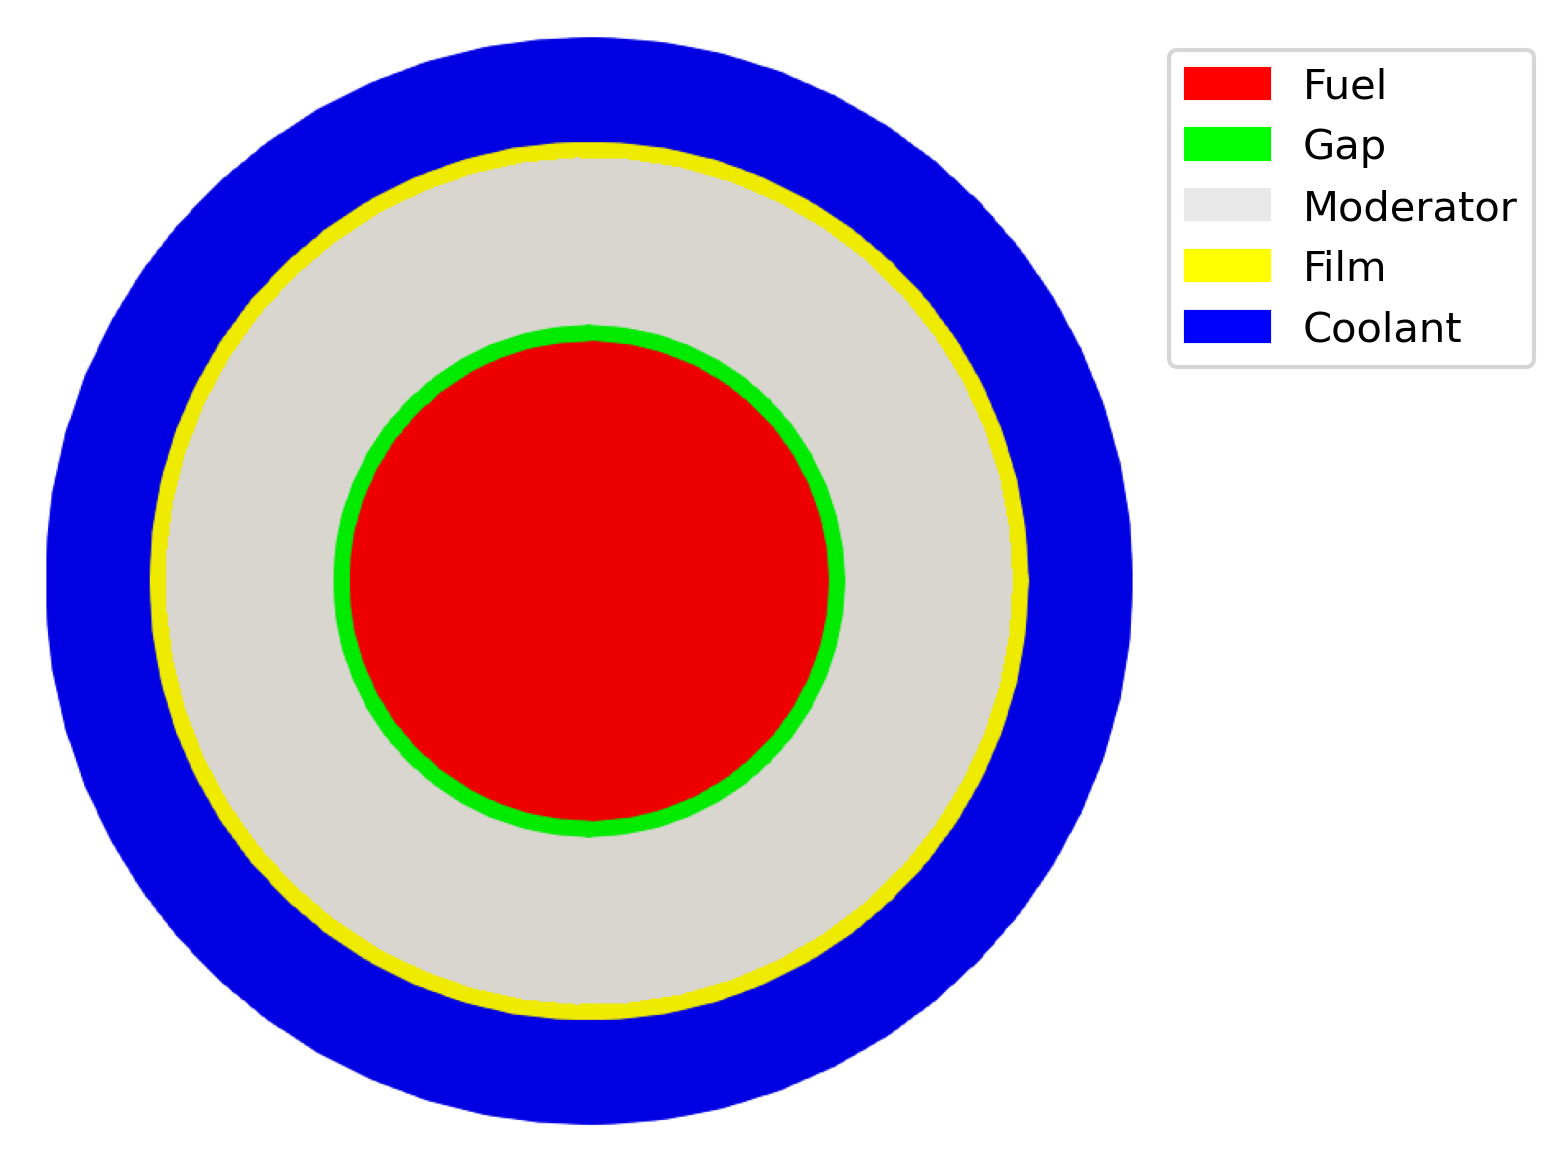
\includegraphics[width=0.40\linewidth]{figures-thermal/ver-mesh2}
	\hfill
	\caption{Model geometry axial layout.}
	\label{fig:th-ver-mesh}
\end{figure}

\begin{table}[htbp!]
\centering
      \caption{Problem characteristics.}
      \label{tab:th-ver-char}
    % \begin{tabular}{@{}l c S[table-format=2.2] c c}
    \begin{tabular}{@{}l c c c c}
    \toprule
    \multicolumn{1}{c}{Parameter} & \multicolumn{1}{c}{Symbol} & \multicolumn{1}{c@{}}{Value} & \multicolumn{1}{c@{}}{Units} & \multicolumn{1}{c}{Reference} \\
    \midrule
  Fuel compact radius       & R$_f$     & 0.6225  & cm       & \cite{in_three-dimensional_2006} \\
  Fuel channel radius       & R$_g$     & 0.6350  & cm       & \cite{in_three-dimensional_2006} \\
  Coolant channel radius    & - 		    & 0.7950  & cm       & \cite{in_three-dimensional_2006} \\
  Fuel/coolant pitch        & -			    & 1.8850  & cm       & \cite{in_three-dimensional_2006} \\
  Fuel column height	      & L 		    & 793 	  & cm 		   & \cite{in_three-dimensional_2006} \\
  Coolant mass flow rate    & $\dot{m}$ & 0.0176  & kg $\cdot s^{-1}$  	& \cite{in_three-dimensional_2006} \\
  Average power density     & q$_{ave}$ & 35      & W $\cdot cm^{-3}$   & \cite{in_three-dimensional_2006} \\
  Coolant inlet temperature & $T_{in}$  & 400     & $^{\circ}C$ & \cite{in_three-dimensional_2006} \\
  Helium inlet pressure     & P 		    & 70      & bar 	      & \cite{in_three-dimensional_2006} \\
  Helium density		        & $\rho_c$  & 4.940 $\times 10^{-6}$ & kg $\cdot cm^{-3}$  & \cite{nist_thermophysical_2020} \\
  Helium heat capacity      & c$_{p,c}$	& 5188    & J $\cdot kg^{-1} \cdot K^{-1}$     & \cite{nist_thermophysical_2020} \\
  Fuel compact thermal conductivity & k$_f$ & 0.07    & W $\cdot cm^{-1} \cdot K^{-1}$ & \cite{tak_numerical_2008} \\
  Gap thermal conductivity  & k$_g$ & 3 $\times 10^{-3}$ & W $\cdot cm^{-1} \cdot K^{-1}$ & \cite{tak_numerical_2008} \\
  Moderator thermal conductivity & k$_m$ & 0.30   & W $\cdot cm^{-1} \cdot K^{-1}$ 	   & \cite{tak_numerical_2008} \\
    \midrule
  \multicolumn{1}{c}{Calculated parameters} &  &  &  & \\  
    \midrule
  Calculated moderator radius  & R$_m$ & 1.080  	& cm    & - \\
  Coolant film radius   		   & R$_{cf}$ & 1.090  	& cm    & - \\
  Calculated coolant radius 	 & R$_c$ & 1.349  	& cm    & - \\
  Coolant average velocity  	 & v$_c$ & 1794.33 	& cm $\cdot s^{-1}$ & - \\
  Film thermal conductivity  	 & k$_{cf}$ & 1.722 $\times 10^{-3}$ & W $\cdot cm^{-1} \cdot K^{-1}$ & - \\
  \bottomrule
  \end{tabular}
\end{table}

Note that this is a simplified model only for verifying that the numerical solution agrees with the analytical solution.
Figure \ref{fig:th-ver-results} shows the axial and radial temperature profiles and demonstrates that both the analytical and numerical solutions exhibit good agreement.
The outlet coolant temperature is 770.2 $^{\circ}$C, whereas maximum fuel temperature is 874.7 $^{\circ}$C.

\begin{figure}[htbp!]
	\centering
    \subfloat[Fuel centerline and bulk coolant axial temperatures.]{
        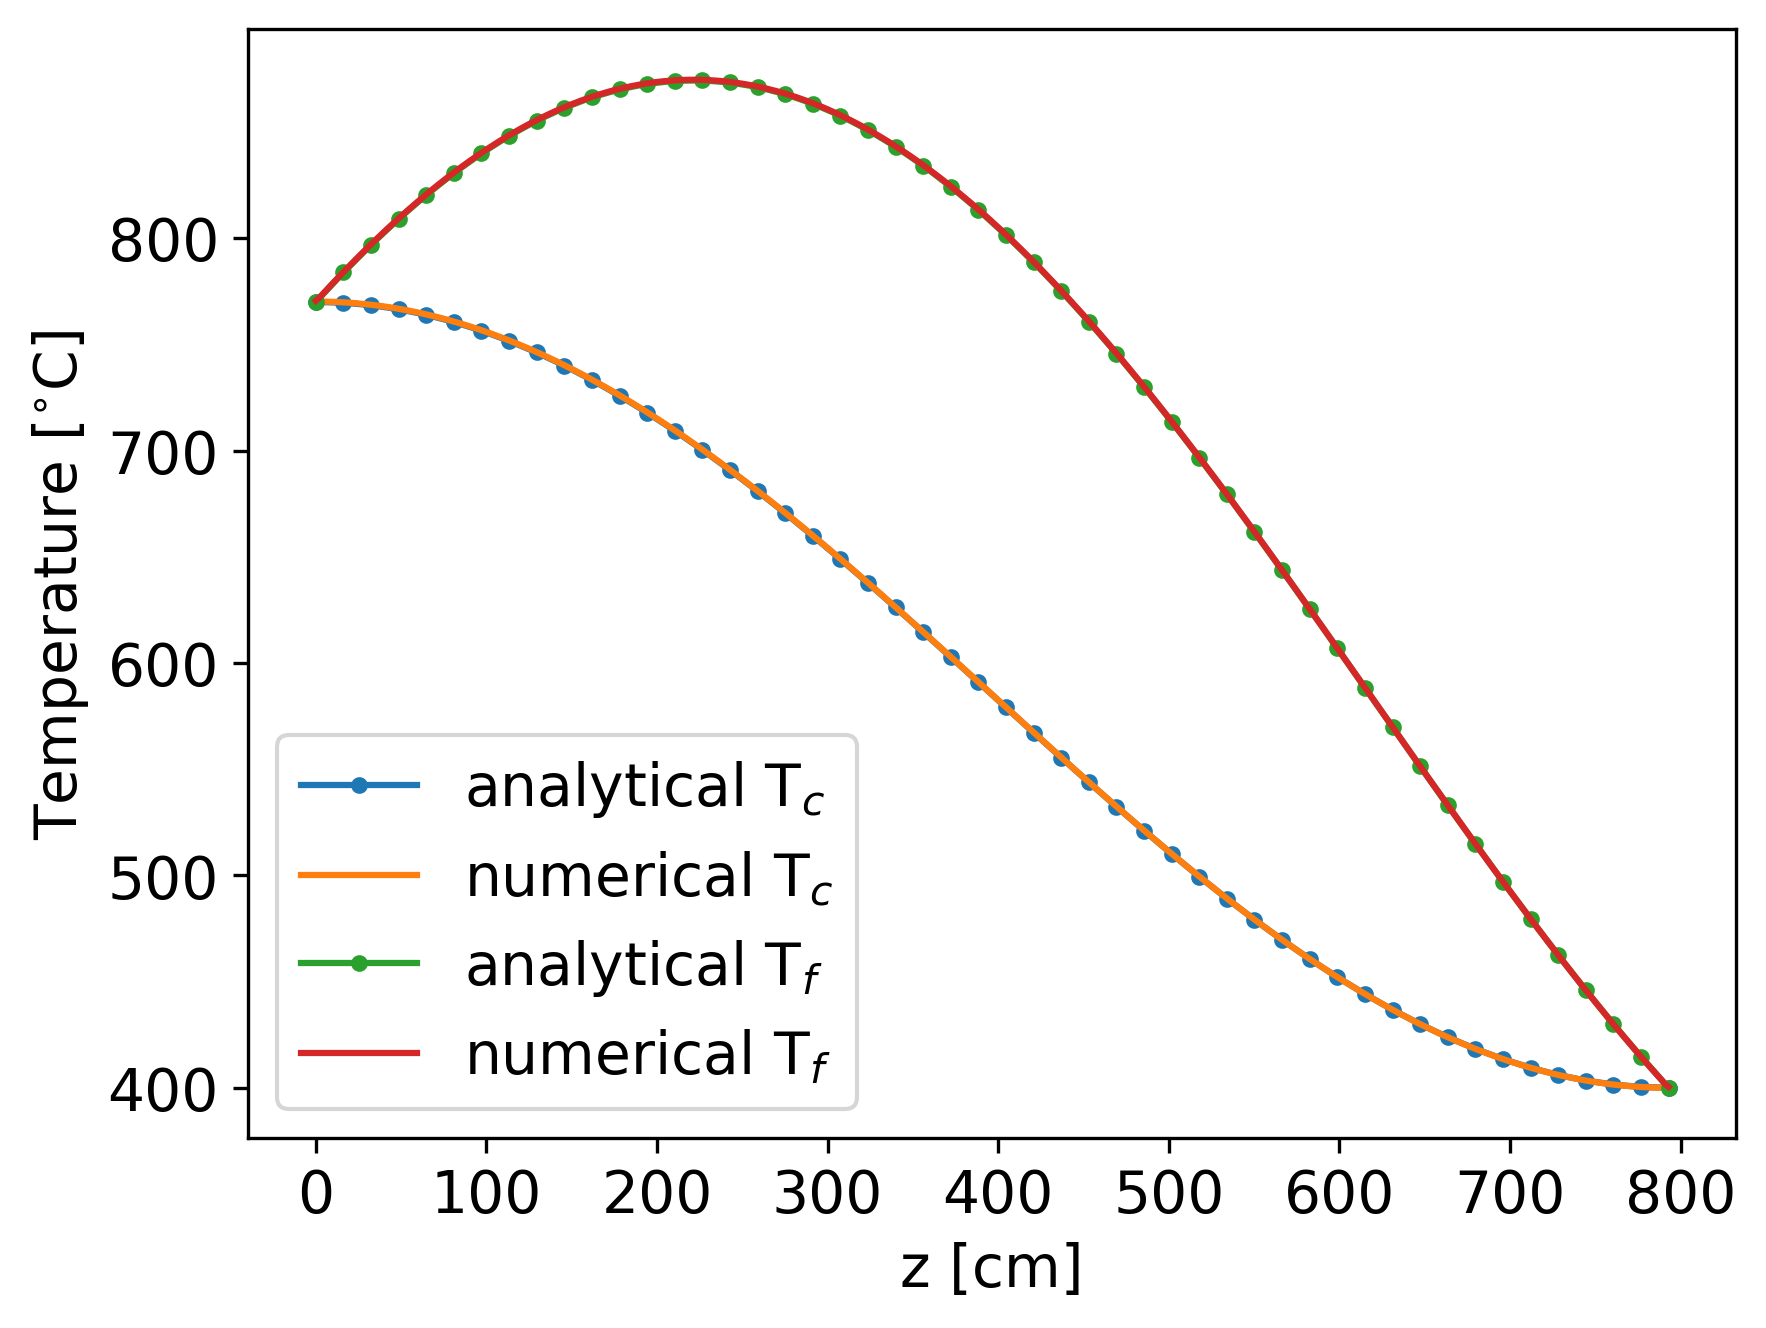
\includegraphics[width=0.45\textwidth]{figures-thermal/2D-preliminar-axial}
    }
    \subfloat[Radial temperature profile at z=L/2=396.5 cm.]{
        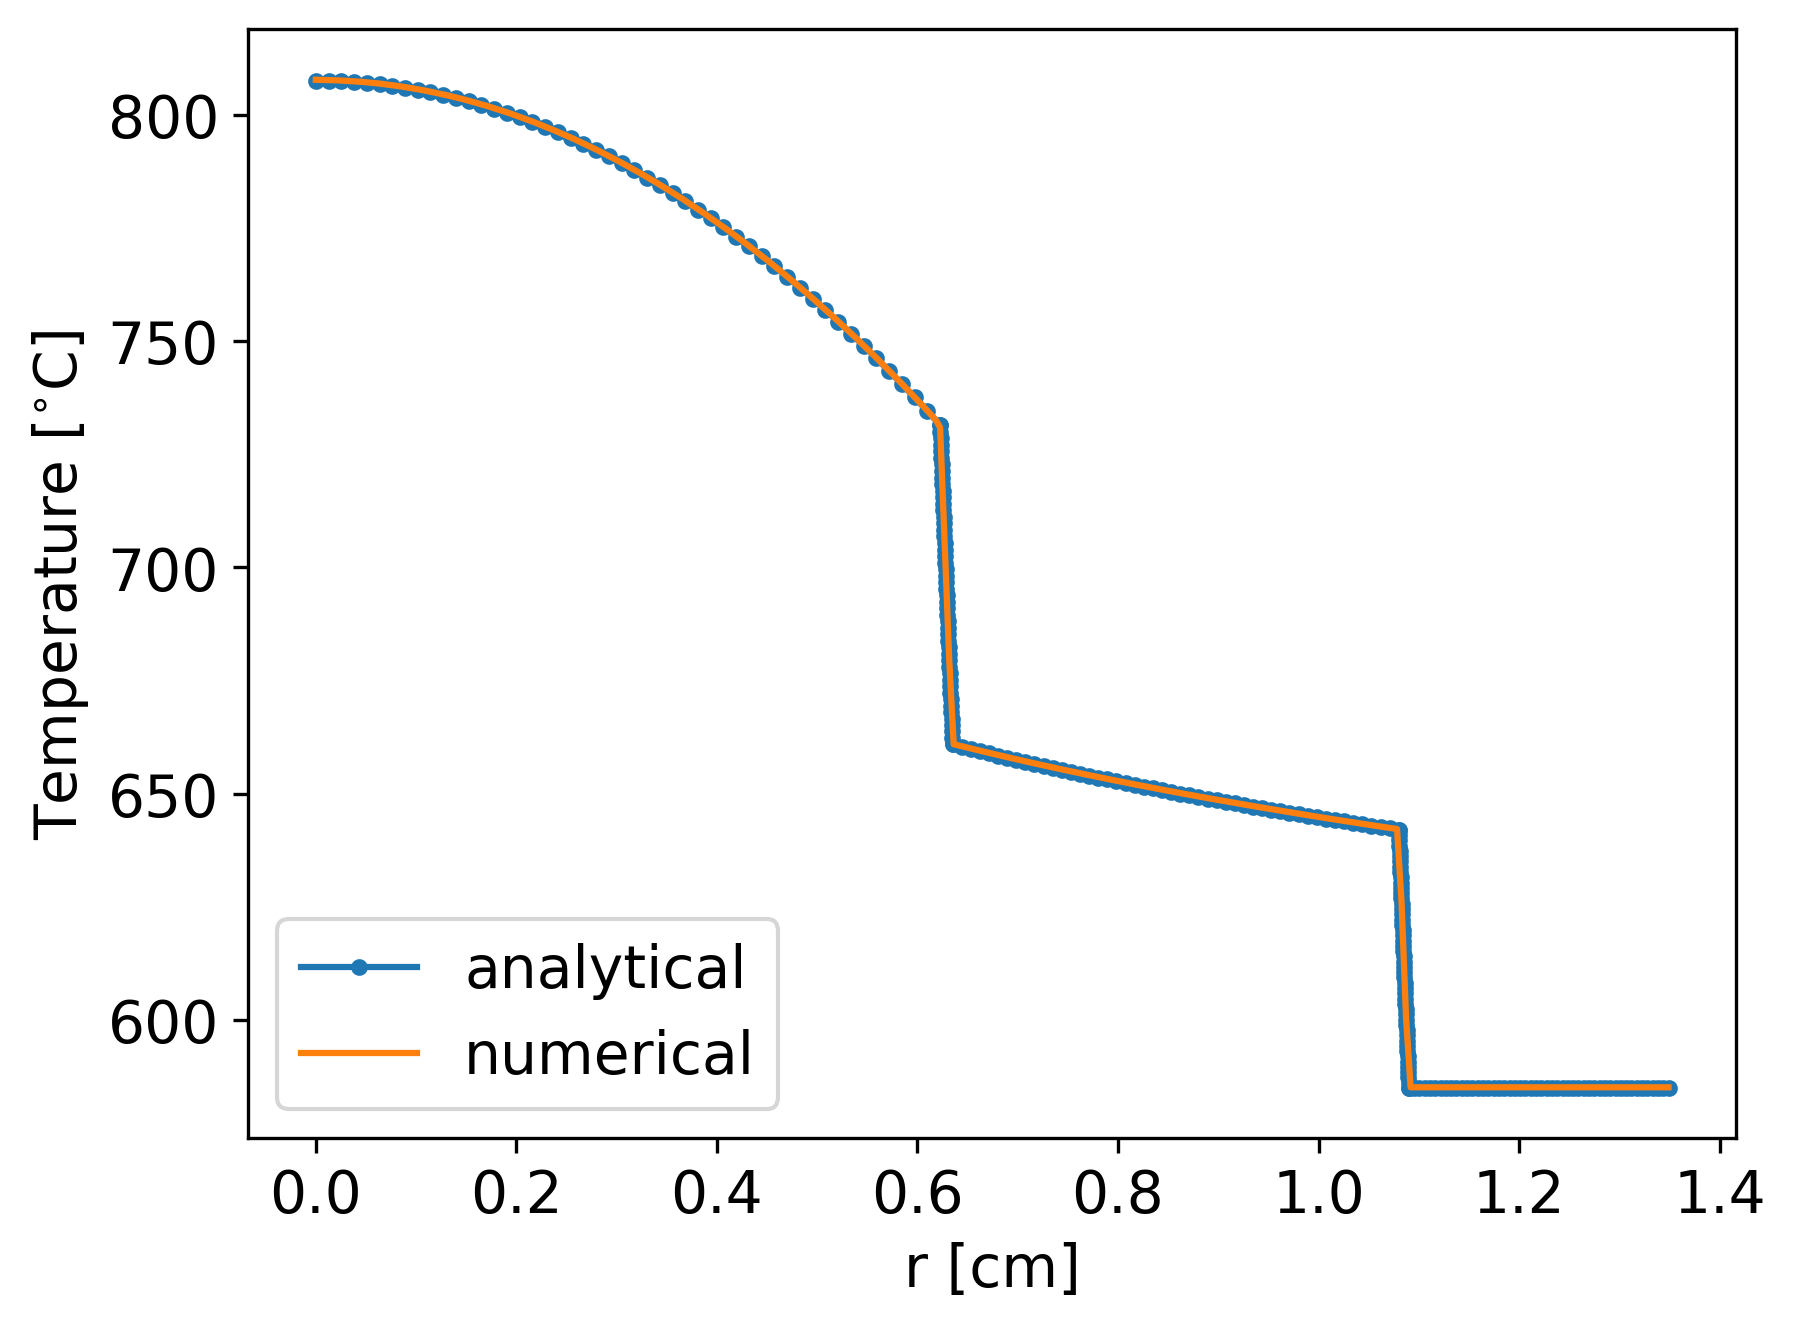
\includegraphics[width=0.45\textwidth]{figures-thermal/2D-preliminar-radial2}
    }
	\hfill
    \caption{Comparison of the analytical and numerical temperature profiles.}
	\label{fig:th-ver-results}
\end{figure}

\subsection{Unit cell problem}
\label{sec:unitcell}

This section solved the unit cell problem in the hot spot of the GT-MHR, which is the spot in the core with the largest power density.
This section intended to reproduce the results found by In et al. 2006 \cite{in_three-dimensional_2006} to validate the unit-cell model.
I chose this article because it solves a three-dimensional unit-cell model and gives one of the most thorough descriptions in the open literature.
Table \ref{tab:th-val-unit-char} presents the problem characteristics.
The article does not specify the solid's material properties, so the model used parameters from Tak et al. 2008 \cite{tak_numerical_2008}.
Figure \ref{fig:th-val-unit-model} displays the model geometry and Figure \ref{fig:th-val-unit-model-b} the temperature dependent material properties.
Additionally, In et al. used a chopped cosine as the power profile, which the model used the average value of to simplify the analysis.

\begin{table}[htbp!]
\centering
      \caption{Problem characteristics.}
      \label{tab:th-val-unit-char}
    % \begin{tabular}{@{}l c S[table-format=2.2] c c}
    \begin{tabular}{@{}l c c c c}
    \toprule
    \multicolumn{1}{c}{Parameter} & \multicolumn{1}{c}{Symbol} & \multicolumn{1}{c@{}}{Value} & \multicolumn{1}{c@{}}{Units} & \multicolumn{1}{c}{Reference} \\
    \midrule
  Fuel compact radius       & R$_f$ & 0.6225    & cm   & \cite{in_three-dimensional_2006} \\
  Fuel channel radius       & R$_g$ & 0.6350    & cm   & \cite{in_three-dimensional_2006} \\
  Coolant channel radius    & R$_c$ & 0.7950    & cm   & \cite{in_three-dimensional_2006} \\
  Fuel/coolant pitch        & p     & 1.8850    & cm   & \cite{in_three-dimensional_2006} \\
  Fuel column height        & L     & 793       & cm   & \cite{in_three-dimensional_2006} \\
  % input parameter characteristics
  Coolant channel mass flow rate & $\dot{m}$ & 0.0176 & kg $\cdot s^{-1}$ & \cite{in_three-dimensional_2006} \\
  Average power density     & q$_{ave}$ & 35    & W $\cdot cm^{-3}$   & \cite{in_three-dimensional_2006} \\
  Inlet coolant temperature & T$_{in}$  & 400   & $^{\circ}$C  & \cite{in_three-dimensional_2006} \\
  Helium inlet pressure & P & 70 & bar & \cite{in_three-dimensional_2006} \\
  Helium density        & $\rho$  & 4.94 $\times 10^{-6}$ & kg $\cdot cm^{-3}$ & \cite{nist_thermophysical_2020} \\
  Helium heat capacity  & c$_p$ & 5188 & J $\cdot kg^{-1} \cdot K^{-1}$ & \cite{nist_thermophysical_2020} \\
    \midrule
  \multicolumn{1}{c}{Calculated parameters} &  &  &  & \\  
    \midrule
  Coolant film radius       & R$_{cf}$ & 0.8050    & cm     & -  \\
  Coolant average velocity  & v$_c$ & 1794.33   & cm $\cdot s^{-1}$   & -  \\
  Film thermal conductivity & k$_{cf}$ & 1.731 $\times 10^{-3}$ & W $\cdot cm^{-1} \cdot K^{-1}$ & -  \\
  \bottomrule
  \end{tabular}
\end{table}

\begin{figure}[htbp!]
  \centering
  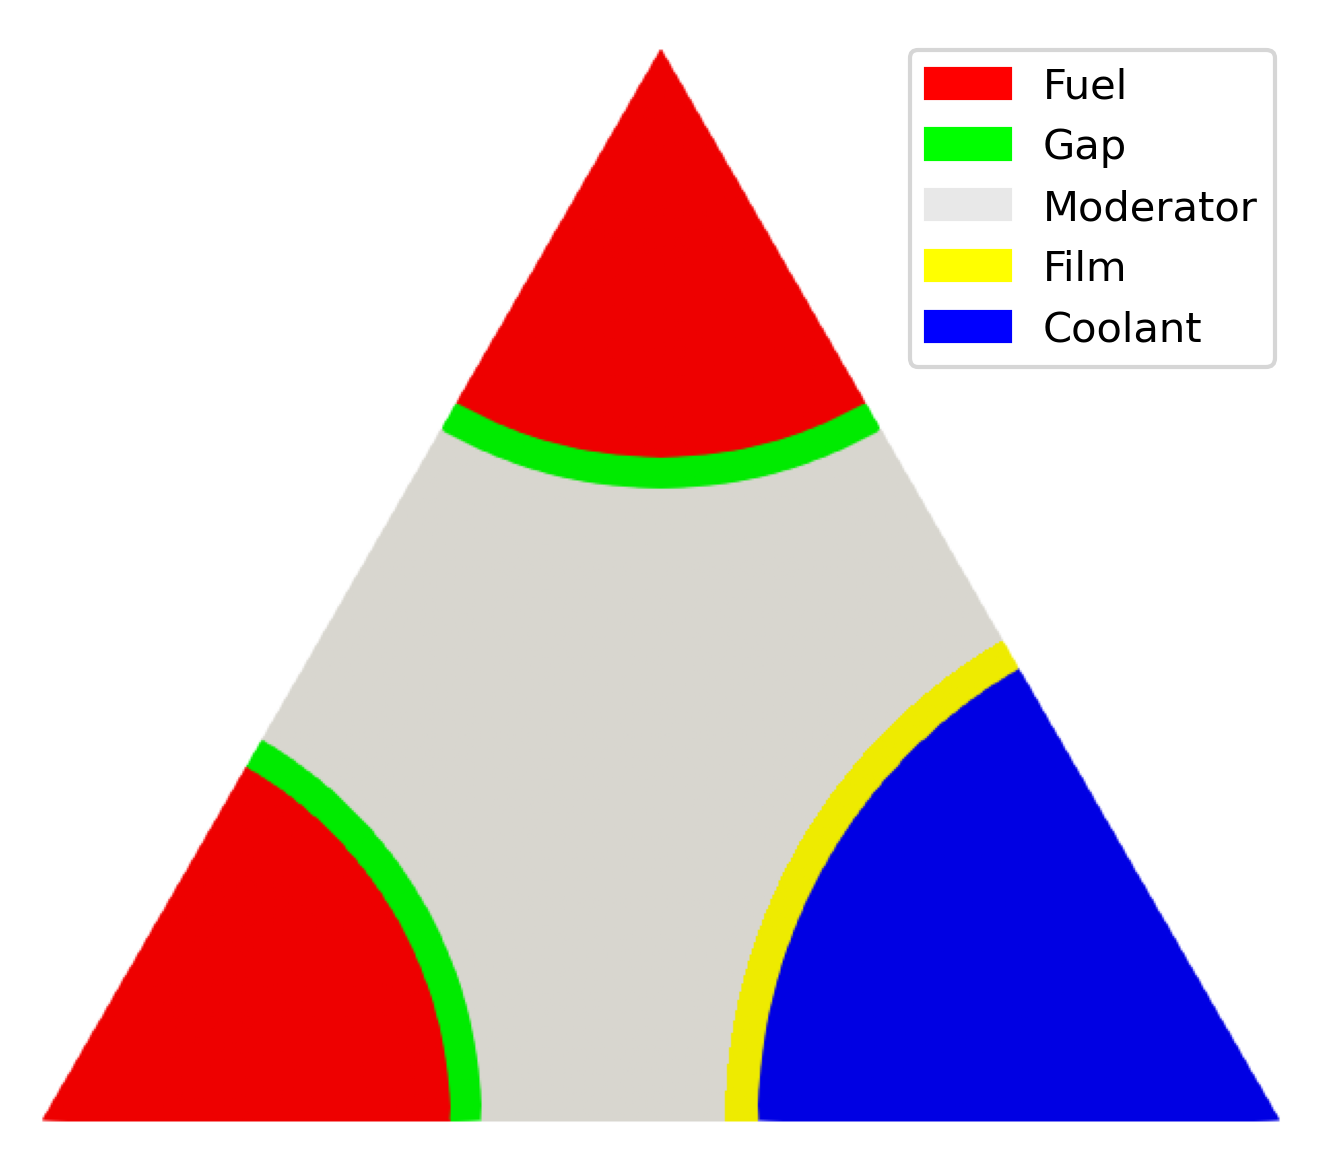
\includegraphics[width=0.40\linewidth]{figures-thermal/unitcell2}
  \hfill
  \caption{Axial layout of the model geometry.}
  \label{fig:th-val-unit-model}
\end{figure}

\begin{figure}[htbp!]
  \centering
  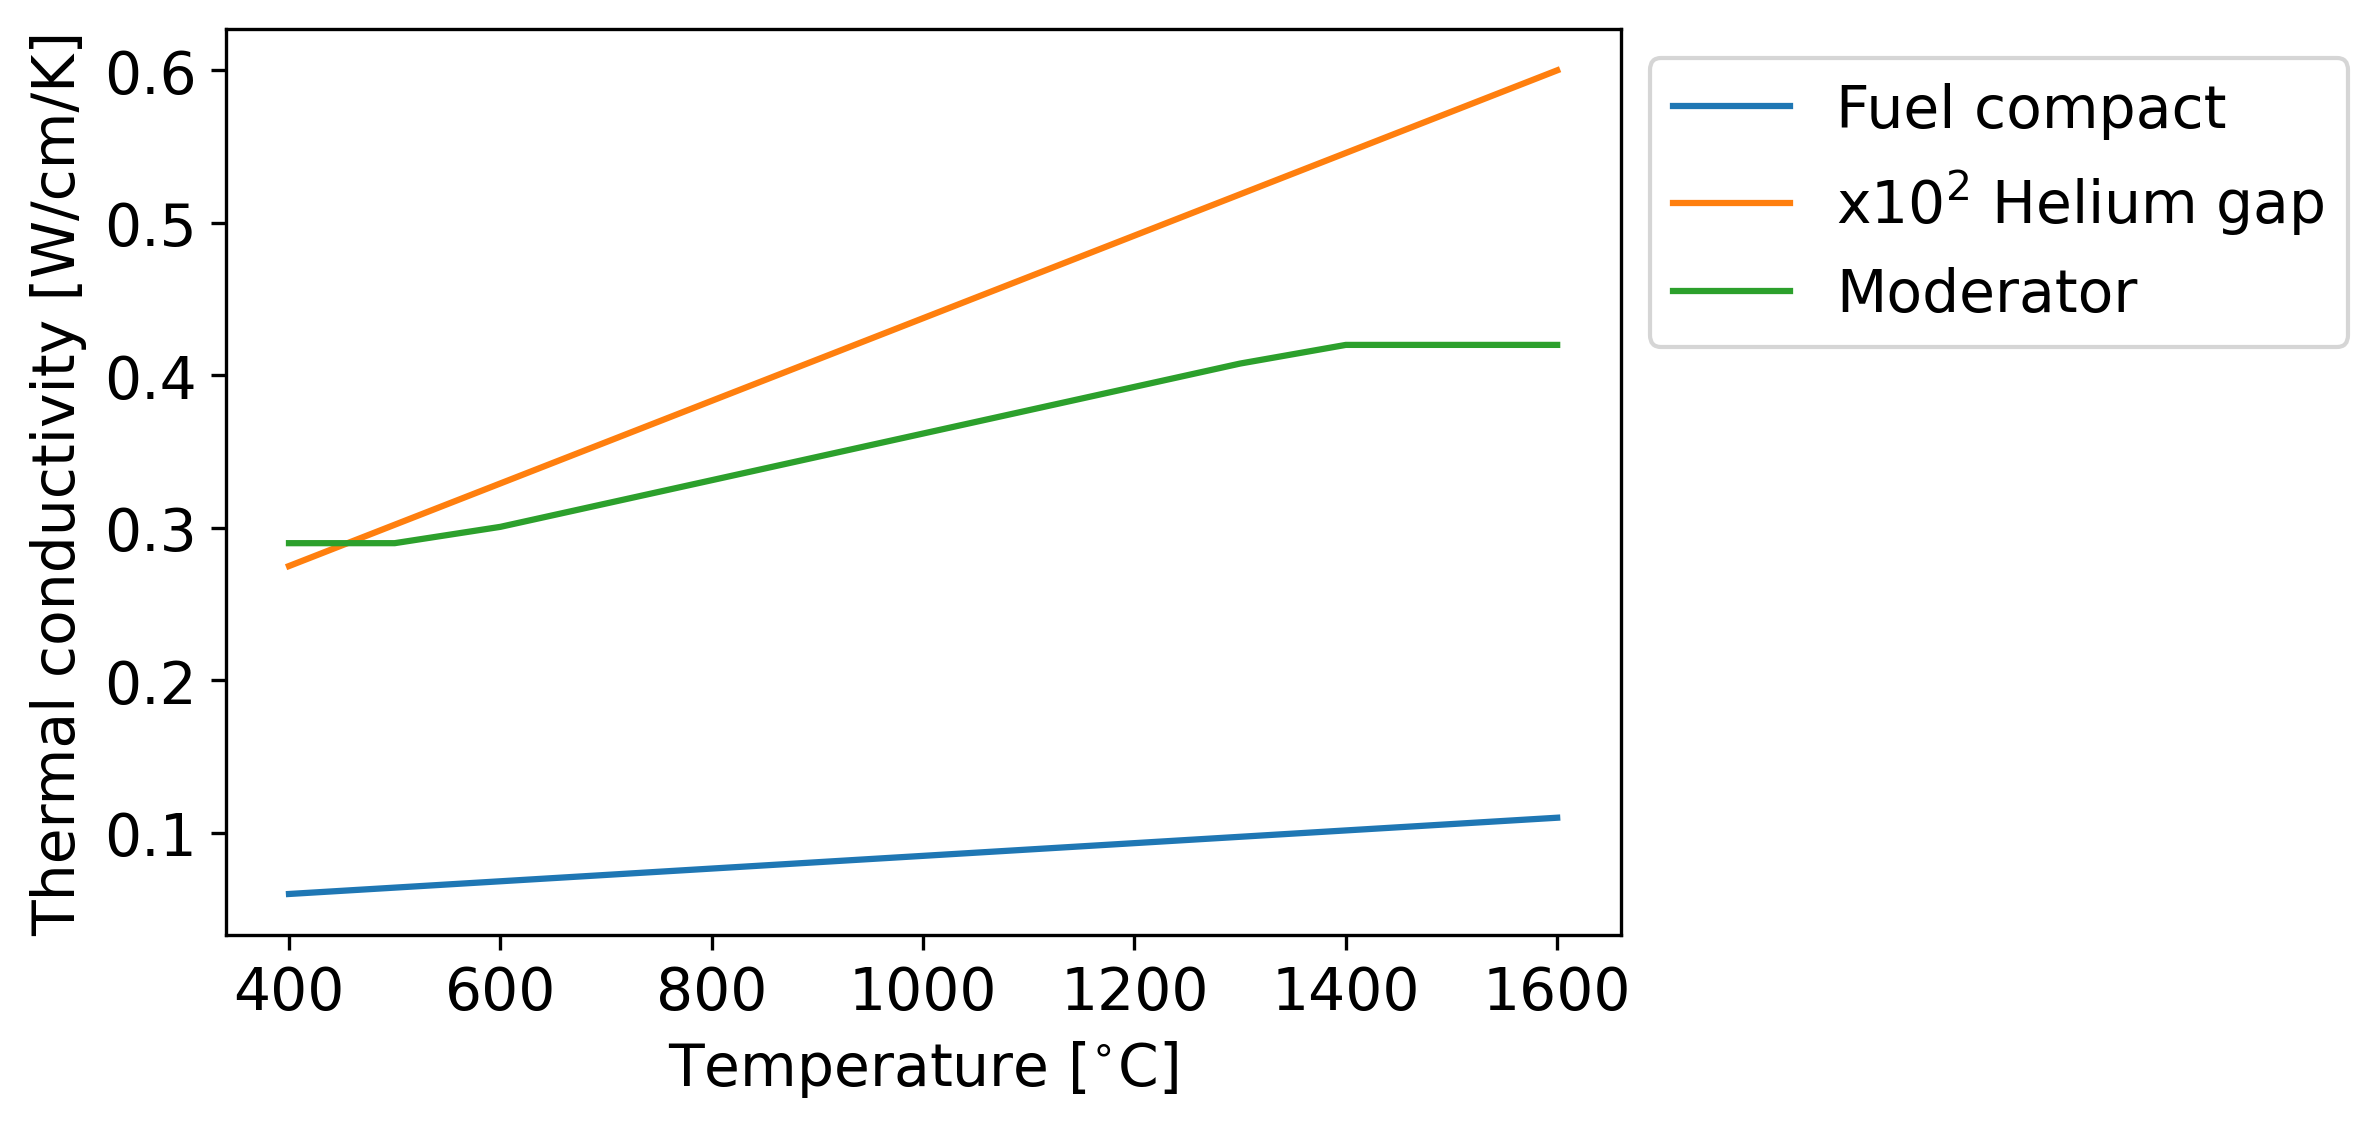
\includegraphics[width=0.40\linewidth]{figures-thermal/val-unit-matprop}
  \hfill
  \caption{Temperature dependent material properties \cite{tak_numerical_2008}.}
  \label{fig:th-val-unit-model-b}
\end{figure}

Figure \ref{fig:th-val-unit-temps} shows the temperature profiles.
From the top to the bottom of the reactor, the axial temperatures increase, the moderator and coolant temperatures remain parallel,
and the difference between the fuel and moderator temperatures decreases.
The model assumes a film thermal conductivity independent of the temperature, thus the moderator and coolant temperature difference is constant.
The solids' thermal conductivity increases with temperature, as shown in Figure \ref{fig:th-val-unit-model-b}, the thermal resistance between the moderator and the fuel decreases, so their temperature difference decreases as well.

Table \ref{tab:th-val-unit-results} summarizes the results.
Equation \ref{eq:rel-error} evaluates the relative difference to the reference results
\begin{align}
  & \Delta_T = \left| \frac{T_M-T_{ref}}{T_{ref}} \right| \cdot 100  \label{eq:rel-error}
  \intertext{where}
  & \Delta_T = \mbox{relative difference } [\%] \notag \\
  & T_M = \mbox{temperature determined by this work} [^{\circ}C] \notag \\
  & T_{ref} = \mbox{reference temperature} [^{\circ}C]. \notag
\end{align}

Small discrepancies arise in the results: Moltres/MOOSE coolant temperature is smaller than In's by 4$^{\circ}$C.
The moderator temperature is larger by 9$^{\circ}$C, and the fuel temperature is larger by 22$^{\circ}$C.
The cause of the fuel temperature discrepancy is the power profile simplification.
As the analysis in the previous section has shown, the fuel-to-coolant temperature difference is small in the outlet for a sinusoidal power profile. 
The opposite extreme scenario is the uniform power profile, where the fuel-to-coolant temperature difference is larger.
In et al. used a chopped cosine power profile, which is between the two former cases.
Hence, this model yields a fuel-to-coolant temperature difference at the outlet larger than In et al.
Overall, Moltres results are close to In's results as the maximum difference between them is 22$^{\circ}$C, which corresponds to less than 2\% relative difference.

\begin{figure}[htbp!]
  \centering
    \subfloat[Maximum fuel, moderator, and bulk coolant axial temperatures.]{
        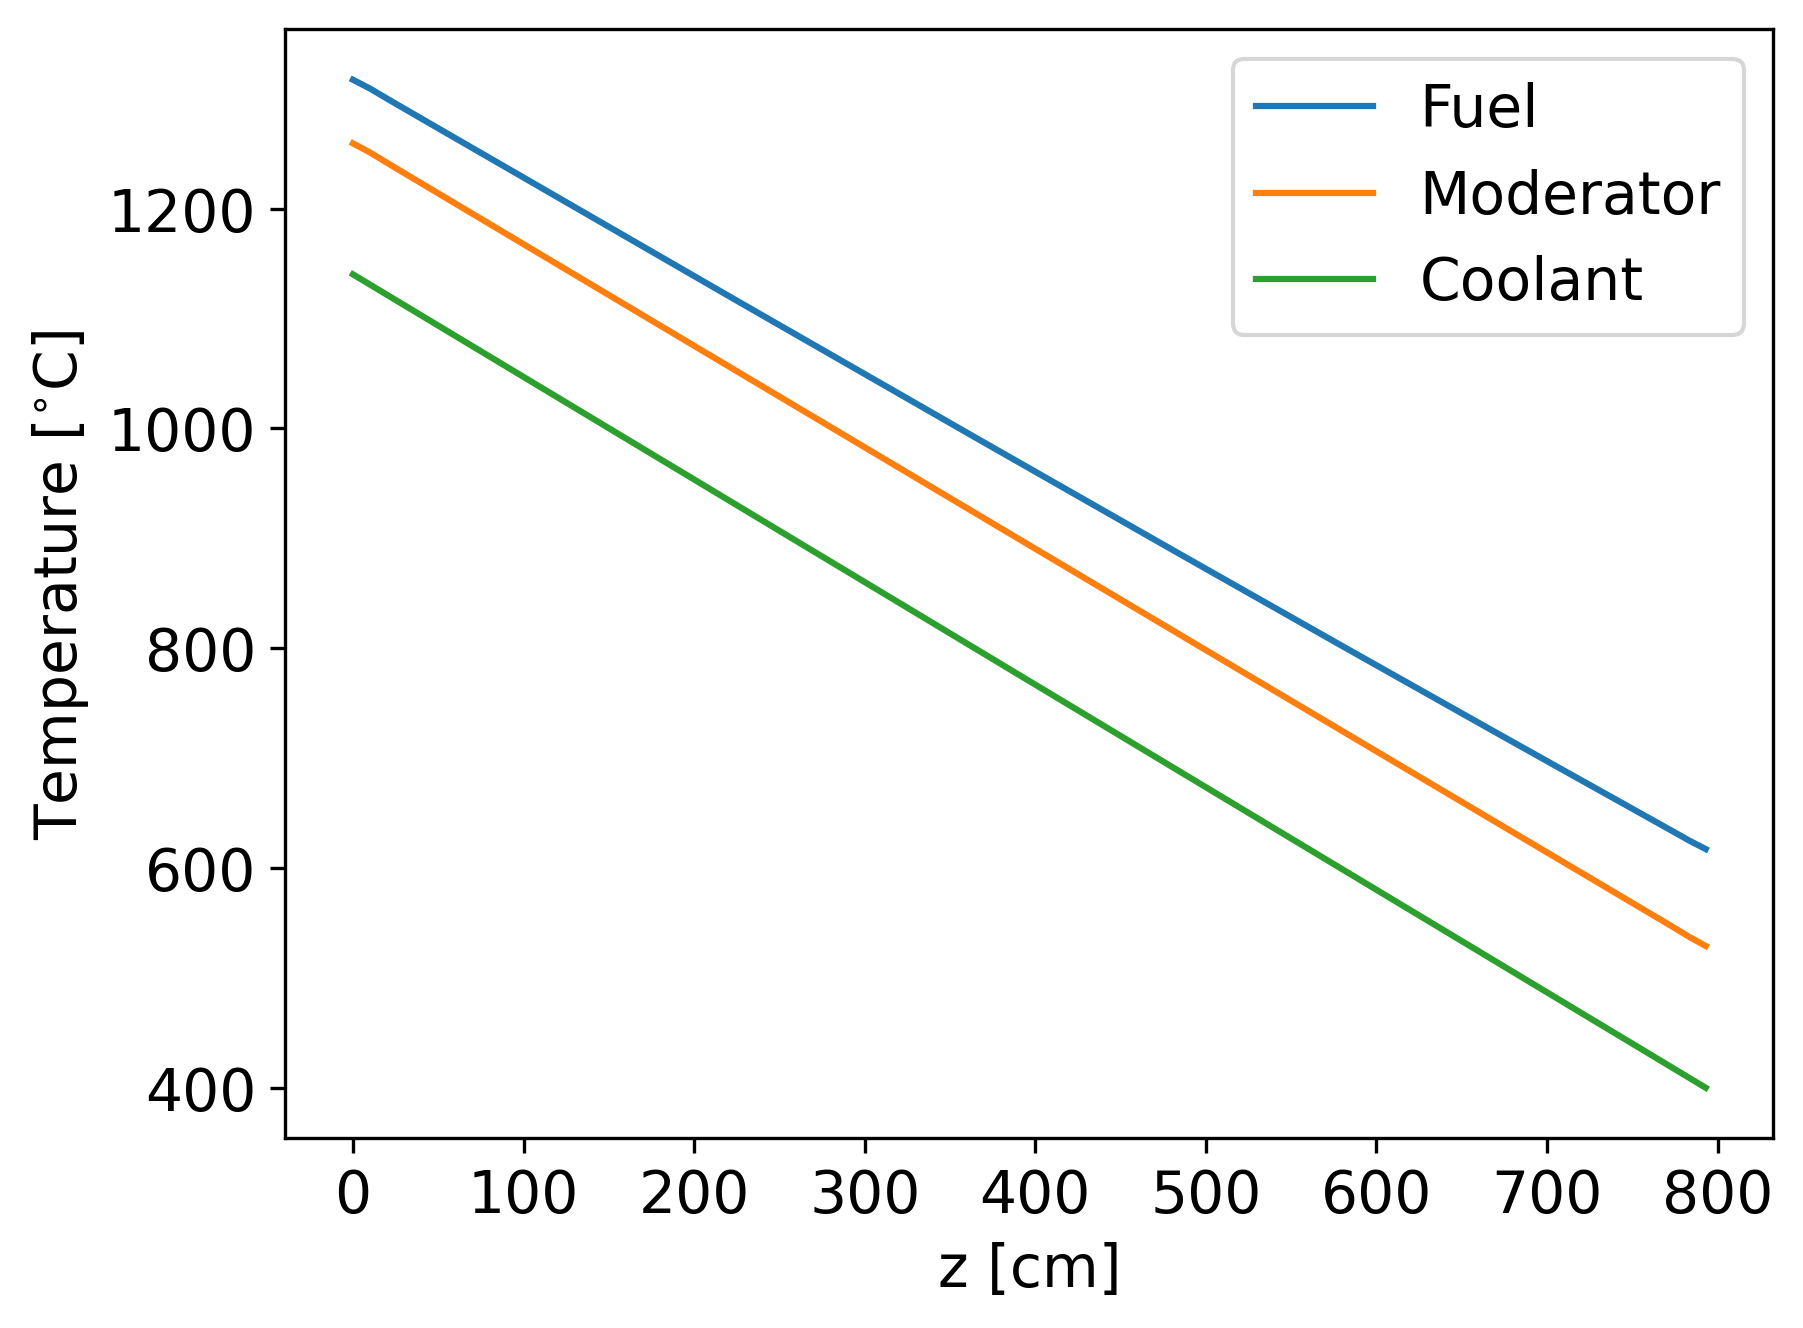
\includegraphics[width=0.45\textwidth]{figures-thermal/in-2006-5-axial}
    }
    \subfloat[Outlet plane (z=793 cm) temperature distribution.]{
        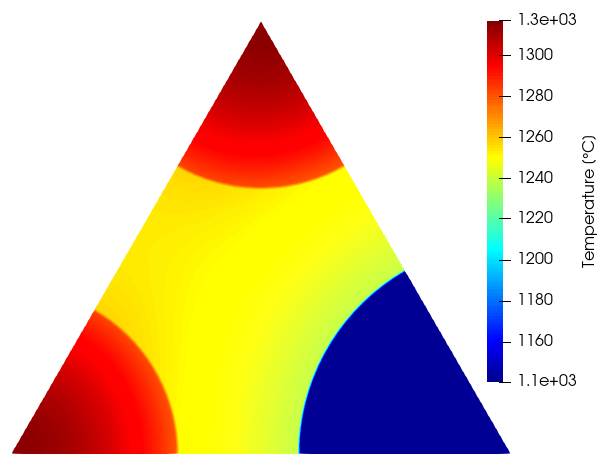
\includegraphics[width=0.45\textwidth]{figures-thermal/val-unit-outlet-plane}
    }
  \hfill
  \caption{Unit cell temperature profile calculated by Moltres.}
  \label{fig:th-val-unit-temps}
\end{figure}

\begin{table}[htbp!]
\centering
    \caption{Comparison between In et al. \cite{in_three-dimensional_2006} and Moltres/MOOSE results.}
    \label{tab:th-val-unit-results}
    \begin{tabular}{@{}l c c c}
    \toprule
  Parameter                      & In et al. [$^{\circ}$C] & Moltres/MOOSE [$^{\circ}$C] & $\Delta_T$ [\%]\\
    \midrule
  Maximum coolant temperature    & 1144      & 1140          & 0.3 \\
  Maximum moderator temperature  & 1250      & 1259          & 0.7 \\
  Maximum fuel temperature       & 1295      & 1317          & 1.7 \\
    \bottomrule
  \end{tabular}
\end{table}

\section{Fuel column}
\label{sec:fuelcol}

This section discusses an HTGR fuel column analysis aimed at validating the fuel column model by reproducing some of Sato et al. 2010 \cite{sato_computational_2010} analyses.
I chose this article because it gives a thorough description of the problem, making it easier to reproduce.
A first analysis studied a column with no bypass-gap between assemblies, while a second analysis studied a column with a 3mm bypass-gap between assemblies.

Figure \ref{fig:th-val-assem-model-a} exhibits the model geometry.
The model only considered a $1/12^{th}$ portion of the column due to symmetry.
The study used the GT-MHR as the reference reactor for the calculations.
The GT-MHR shares the geometry dimensions with the MHTGR, which Table \ref{tab:element-characteristics} specifies.

\begin{figure}[htbp!]
  \centering
  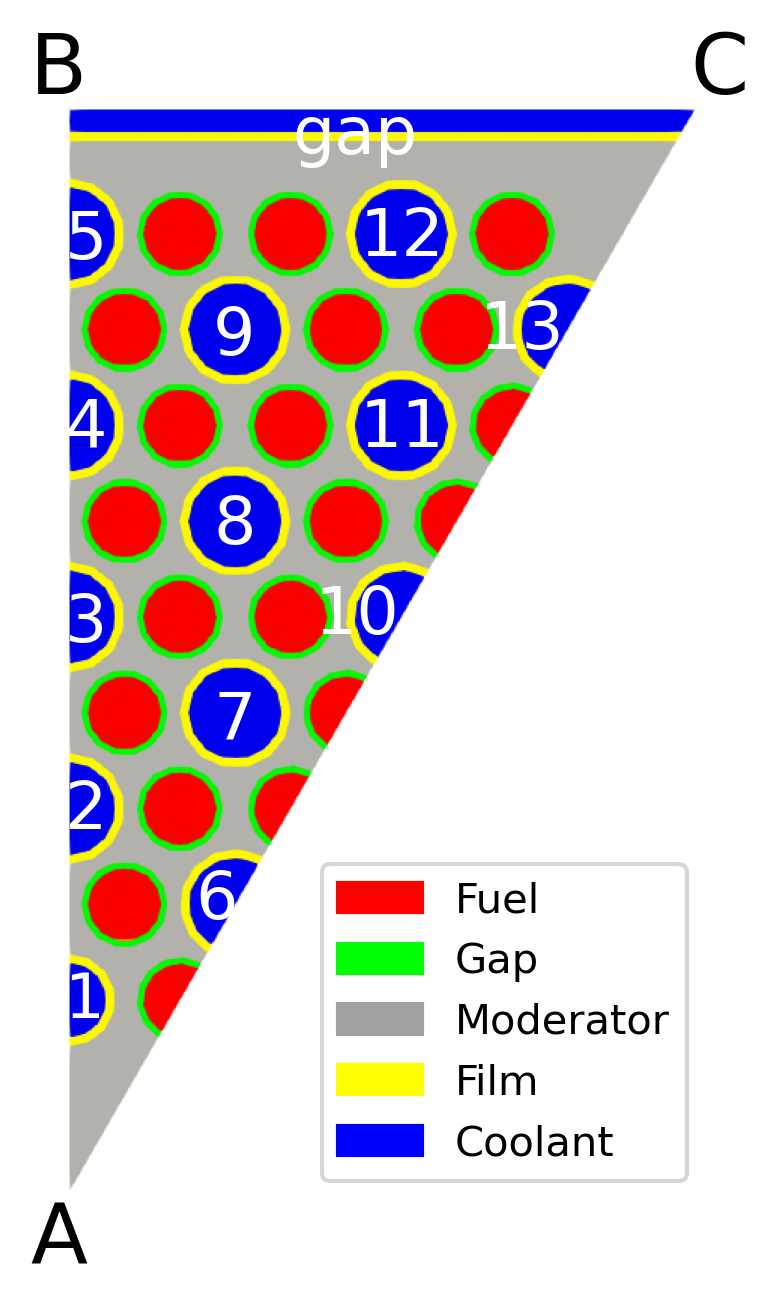
\includegraphics[width=0.25\linewidth]{figures-thermal/val-assem-mesh}
  \hfill
  \caption{Model geometry axial layout.}
  \label{fig:th-val-assem-model-a}
\end{figure}

Equation \ref{eq:matcoeff} evaluates the solid material properties \cite{johnson_cfd_2009}
\begin{align}
  \phi(T) = A_1 + A_2 T + A_3 T^2 + A_4 T^3 + A_5 T^4.  \label{eq:matcoeff}
\end{align}

Table \ref{tab:th-val-assem-mat} displays the fuel compact and moderator coefficients of equation \ref{eq:matcoeff}.
% Figure \ref{fig:th-val-assem-model-b} shows the temperature-dependent material properties.

\begin{table}[htbp!]
\centering
  \caption{Thermal conductivity coefficients \cite{johnson_cfd_2009}.}
  \label{tab:th-val-assem-mat} 
  \begin{tabular}{c| S[table-format=2.2] S[table-format=2.2e-1] S[table-format=3.3] |S[table-format=2.2e-1]}
  % \begin{tabular}{c|ccc|c}
\toprule
                          & \multicolumn{3}{c|}{Moderator} & \multicolumn{1}{c}{Fuel compact} \\
Temperature range {[}K{]} & \multicolumn{1}{c}{255.6-816} & \multicolumn{1}{c}{816-1644.4} & \multicolumn{1}{c|}{1644.4-1922.2} & \multicolumn{1}{c}{255.6-2200}   \\
\midrule
A1                        & 28.6      & 1.24e+2   & 41.5         & 3.94         \\
A2                        &          & -3.32e-1   &              & 3.59e-3      \\
A3                        &          & 4.09e-4    &              & -1.98e-9     \\
A4                        &          & -2.11e-7   &              & 3.19e-12     \\
A5                        &          & 4.02e-11   &              & -9.77e-16    \\
\bottomrule
  \end{tabular}
\end{table}

% \begin{figure}[htbp!]
%   \centering
%   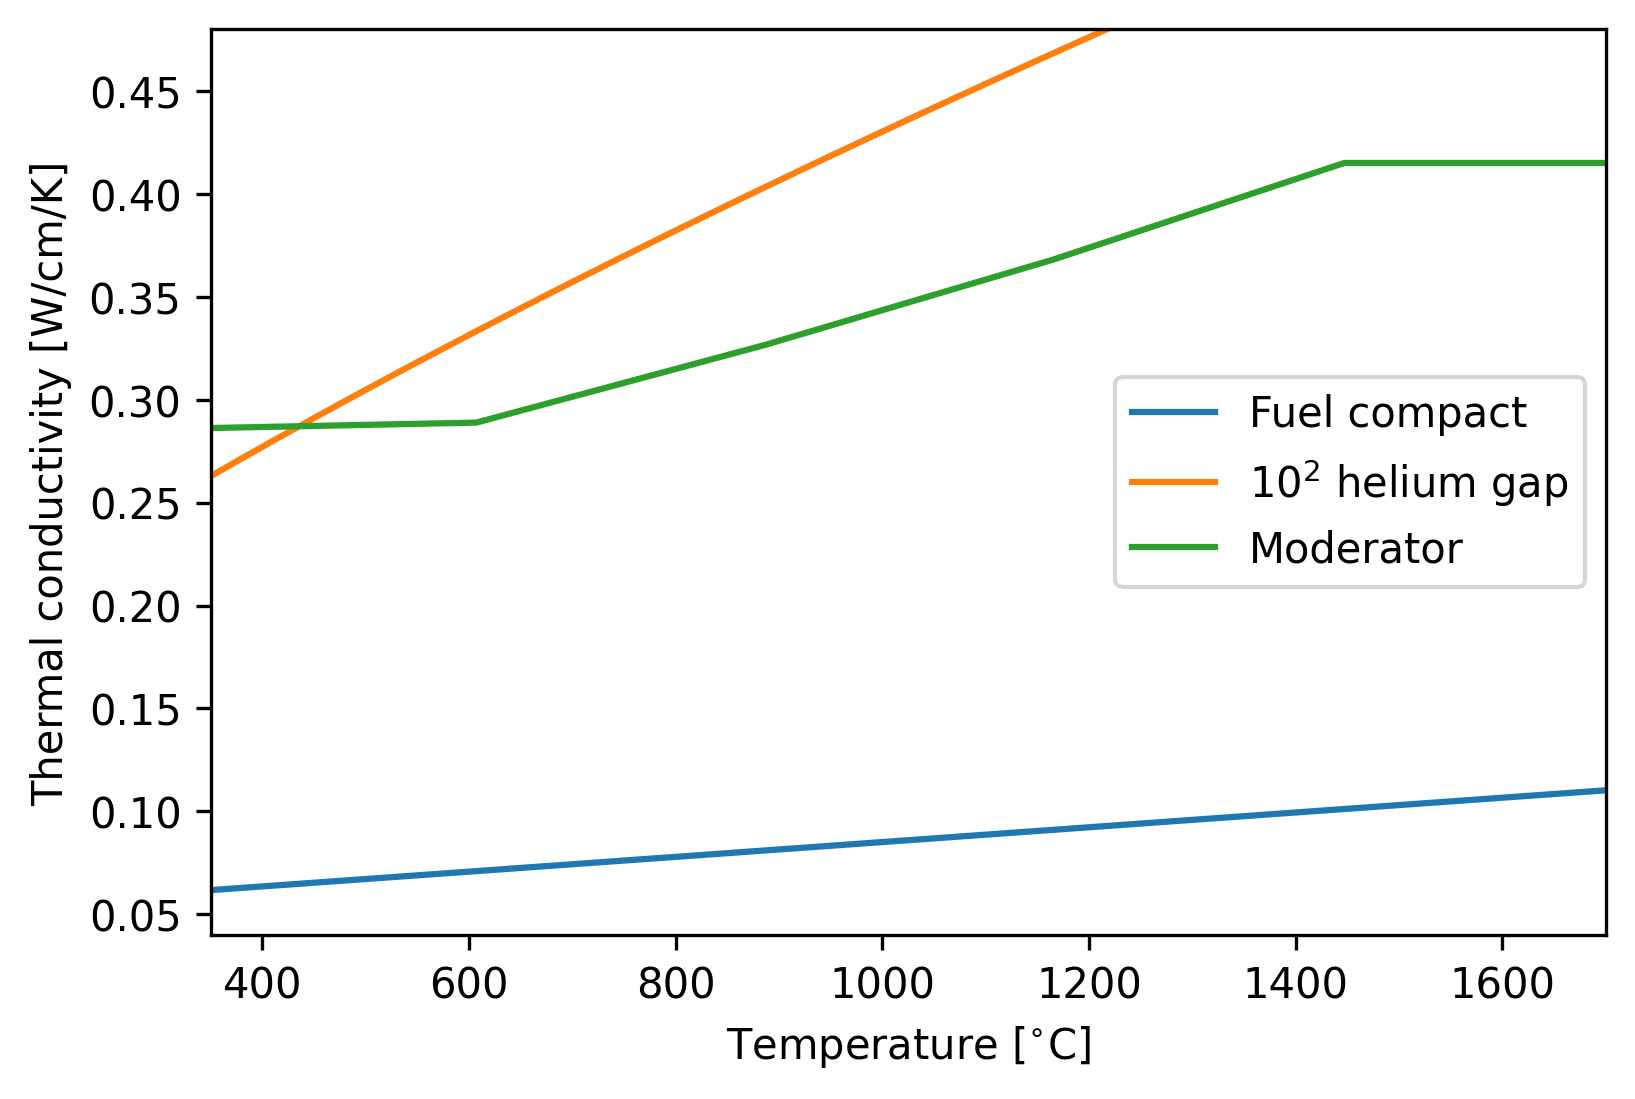
\includegraphics[width=0.45\linewidth]{figures-thermal/val-assem-matprop}
%   \hfill
%   \caption{Temperature dependent material properties \cite{johnson_cfd_2009}.}
%   \label{fig:th-val-assem-model-b}
% \end{figure}

Table \ref{tab:th-val-assem-char} lists the remaining input parameters.
The model assigns a number to each coolant channel and the bypass-gap (see Figure \ref{fig:th-val-assem-model-a}).
the calculations used the mass flow distribution from Sato et al \cite{sato_computational_2010}.
Table \ref{tab:th-val-assem-massflow} shows the mass flow rate in each channel.

\begin{table}[htbp!]
\centering
      \caption{Constant problem characteristics.}
      \label{tab:th-val-assem-char}
    % \begin{tabular}{@{}l c S[table-format=2.2] c c}
    \begin{tabular}{@{}l c c c c}
    \toprule
    \multicolumn{1}{c}{Parameter} & \multicolumn{1}{c}{Symbol} & \multicolumn{1}{c@{}}{Value} & \multicolumn{1}{c@{}}{Units} & \multicolumn{1}{c}{Reference} \\
    \midrule
  Inlet coolant temperature & T$_{in}$  & 490   & $^{\circ}$C   & \cite{sato_computational_2010} \\
  Helium inlet pressure     & P         & 70    & bar           & \cite{sato_computational_2010} \\
  Helium density            & $\rho$    & 4.37 $\times 10^{-6}$ & kg $\cdot cm^{-3}$ & \cite{nist_thermophysical_2020} \\
  Helium heat capacity      & c$_p$     & 5188  & J $\cdot kg \cdot K$      & \cite{nist_thermophysical_2020} \\
  Average power density     & q$_{ave}$ & 27.88 & W $\cdot cm^{-3}$         & \cite{sato_computational_2010} \\
    \midrule
  \multicolumn{1}{c}{Calculated parameters} &  &  &  & \\  
    \midrule
  Coolant film radius       & R$_{cf}$ & 0.804     & cm     & -  \\
  Film thermal conductivity & k$_{cf}$ & 2.09 $\times 10^{-3}$ & W $\cdot cm^{-1} \cdot K^{-1}$ & -  \\
  \bottomrule
  \end{tabular}
\end{table}

\begin{table}[htbp!]
\centering
  \caption{Mass flow rate determined from Sato calculation \cite{sato_computational_2010}. Values expressed in [g/s].}
  \label{tab:th-val-assem-massflow}
  \begin{tabular}{l|ccccccc}
\toprule
Channel & 1 & 2 & 3 & 4 & 5 & 6 & 7 \\
\midrule
No bypass-gap  & 6.18 & 11.34 & 11.37 & 11.38 & 11.43 & 11.33 & 22.70 \\
3mm bypass-gap & 5.88 & 10.80 & 10.85 & 10.91 & 11.08 & 10.80 & 21.58 \\
\midrule
Channel & 8 & 9 & 10 & 11 & 12 & 13 & Gap \\
\midrule
No bypass-gap  & 22.73 & 22.73 & 11.38 & 22.77 & 22.91 & 11.44 & -     \\
3mm bypass-gap & 21.67 & 21.83 & 10.88 & 21.81 & 22.20 & 11.10 & 16.56 \\
\bottomrule
\end{tabular}
\end{table}

Table \ref{tab:th-val-assem-results} compares the results determined in this thesis using Moltres/MOOSE to Sato's results \cite{sato_computational_2010}.
In the case with no bypass-gap, Moltres/MOOSE's maximum coolant temperature is 2 $^{\circ}$C lower, and the maximum fuel temperature is 4$^{\circ}$C higher.
In the case with a 3mm bypass-gap, Moltres/MOOSE's maximum coolant temperature is 2 $^{\circ}$C lower, and the maximum fuel temperature is 1$^{\circ}$C lower.
The results showed good agreement with those in \cite{sato_computational_2010}.

Figure \ref{fig:th-val-assem-temps} displays the outlet temperature along lines A-B and A-C from Figure \ref{fig:th-val-assem-model-a}.
The temperature is higher closer to the column center, because the bypass-flow causes the temperature in the center to rise while reducing the peripheral temperature.
The presence of the gap between assemblies produces a larger temperature gradient in the assembly.

\begin{table}[htbp!]
  \centering
  \caption{Comparison of the maximum temperatures calculated by this work and the reference values from Sato et al. \cite{sato_computational_2010}. Temperature values expressed in [$^{\circ}$C].}
  \label{tab:th-val-assem-results}
\begin{tabular}{lcccccc}
\toprule
        & \multicolumn{3}{c}{No gap} & \multicolumn{3}{c}{3mm gap} \\
\midrule
        & $T_{ref}$ & Moltres/MOOSE  & $\Delta_T$ [\%] & $T_{ref}$ & Moltres/MOOSE & $\Delta_T$ [\%] \\
\midrule
Coolant & 985       & 983   & 0.2    & 1007      & 1005 & 0.2   \\  
Fuel    & 1090      & 1094  & 0.4    & 1115      & 1114 & 0.1   \\
\bottomrule
\end{tabular}
\end{table}

\begin{figure}[htbp!]
  \centering
  % \hspace*{\fill}
    \subfloat[Line A-B.]{
        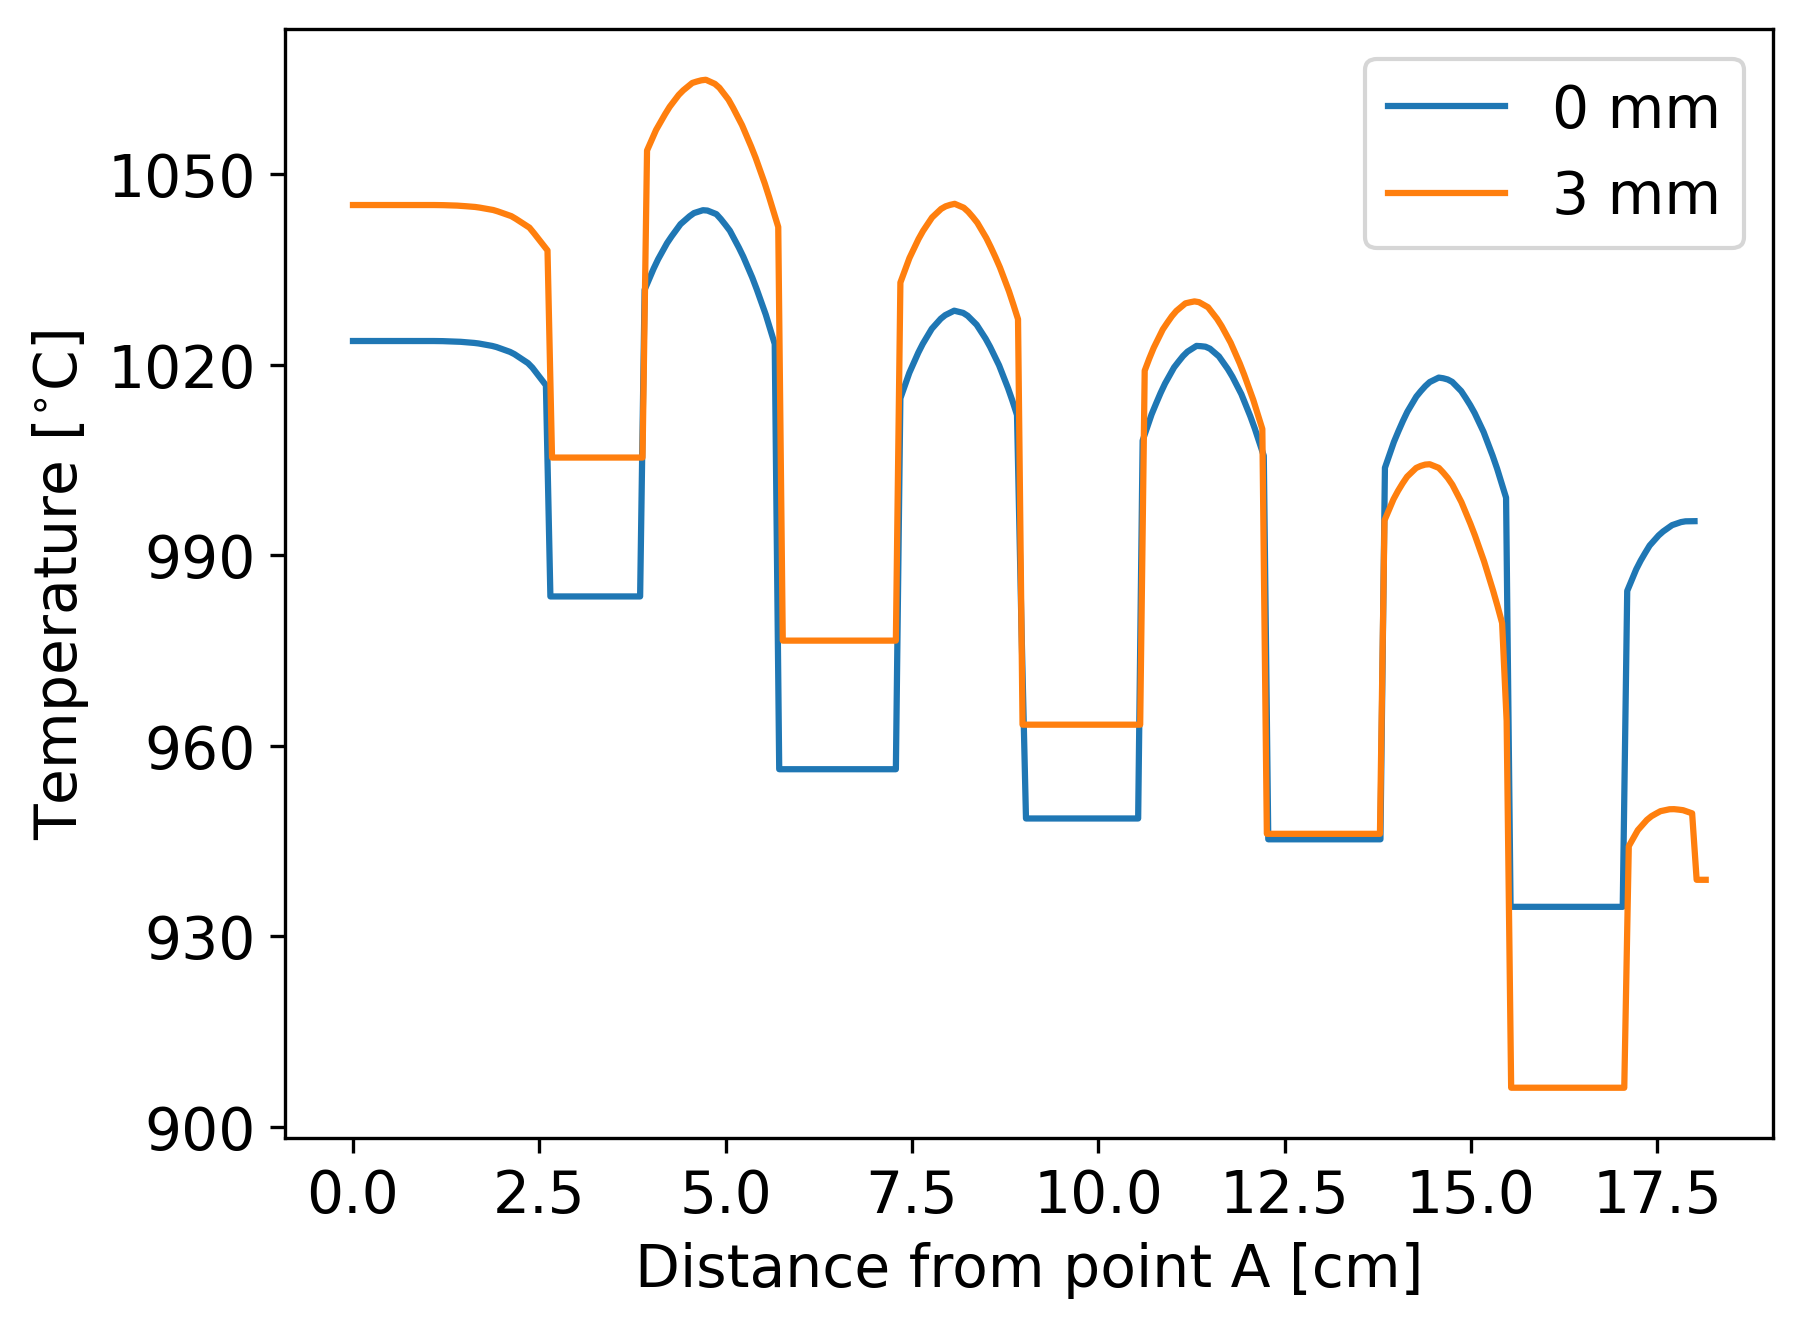
\includegraphics[width=0.45\textwidth]{figures-thermal/val-assem-line-AB}
    }
    \subfloat[Line A-C.]{
        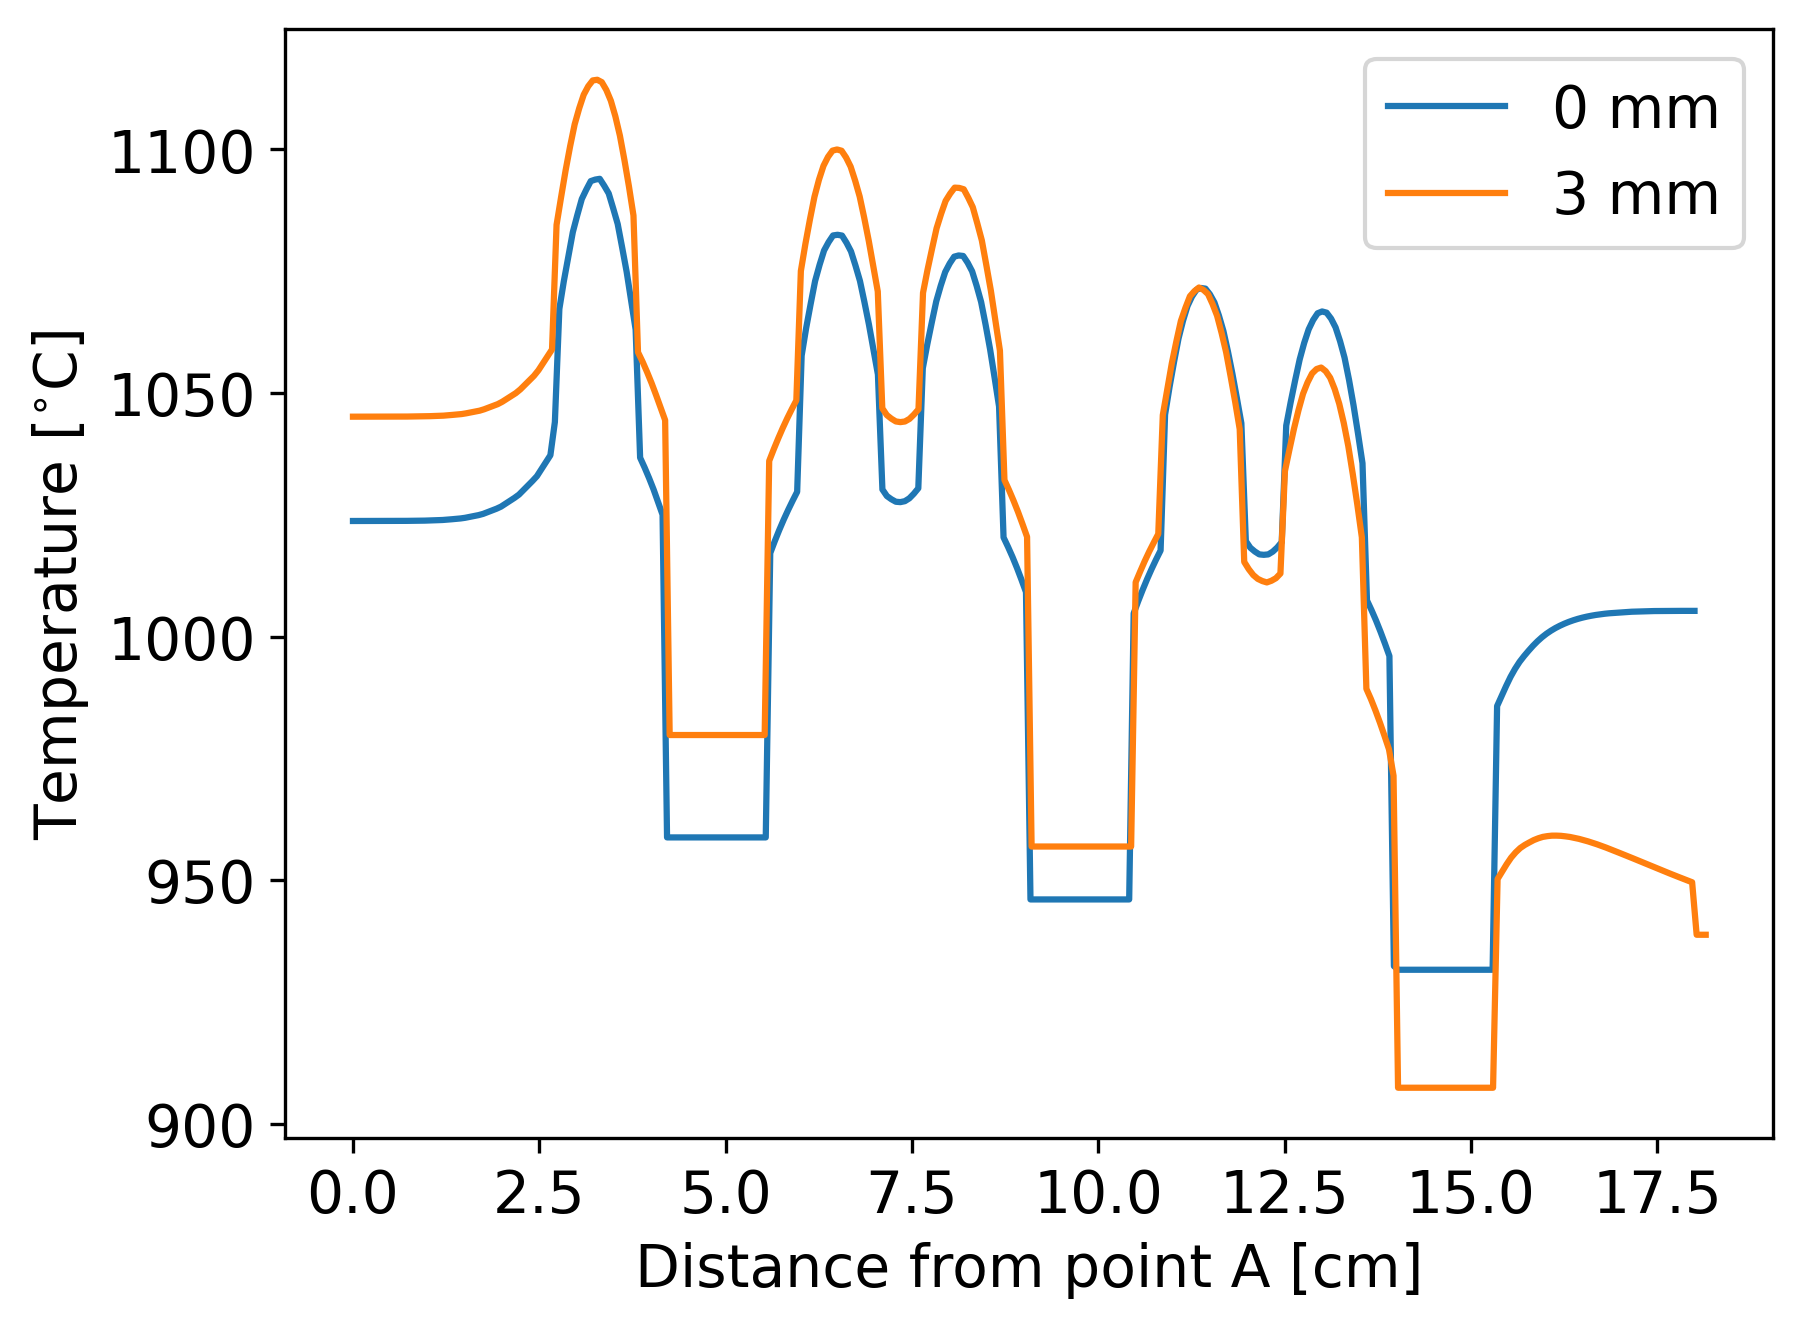
\includegraphics[width=0.45\textwidth]{figures-thermal/val-assem-line-AC}
    }
  \hfill
  \caption{Outlet plane temperature along the line A-B and line A-C.}
  \label{fig:th-val-assem-temps}
\end{figure}

\subsection{Flow distribution analysis}
\label{sec:flowdistrib}

As described in Section \ref{sec:litrev-thermalf}, several methods are available to calculate the flow distribution in prismatic HTGRs.
This section compares a few such methods.
The metrics chosen for this comparison are the maximum coolant and fuel temperatures and the mass flow distribution.
The model assigns a number to each coolant channel and the bypass-gap (see Figure \ref{fig:th-val-assem-model-a}).
Note that Channel 1 is a small coolant channel while Channels 2 to 13 are large coolant channels.

This study used the mass flow distribution from Sato et al. \cite{sato_computational_2010} and analyzed the following cases:
\begin{itemize}
    \item Case 1: uses a flat velocity profile (every channel and gap has the same velocity).
    \item Case 2: uses the incompressible flow model with temperature-independent helium viscosity.
    \item Case 3: uses the incompressible flow model with a temperature-dependent helium viscosity.
    \item Case 4: uses the low-Mach number model with a temperature dependent helium viscosity.
\end{itemize}

Case 1 assumes a flat velocity profile in all coolant paths and calculated the mass flow using equation \ref{eq:case1mdot}
\begin{align}
  & \dot{m}_i = \frac{A_i}{\sum_j A_j} \dot{m}_T \label{eq:case1mdot}
  \intertext{where}
  & \dot{m}_i = \mbox{channel $i$ mass flow rate } [kg \cdot s^{-1}] \notag \\
  & A_i = \mbox{channel $i$ cross-sectional area } [cm^2] \notag \\
  & \dot{m}_T = \mbox{total mass flow rate } [kg \cdot s^{-1}]. \notag
\end{align}

Case 2 and 3 used equation \ref{eq:case2mdot} \cite{melese_thermal_1984} to calculate the pressure drop
\begin{align}
  & \Delta P = \frac{\dot{m}_i^2}{\rho_i A_i^2} f \frac{2 L}{D_h} \label{eq:case2mdot} \\
  & B_i = \frac{1}{\rho_i A_i^2} f \frac{2 L}{D_h}
  \intertext{where}
%  & \dot{m}_i = \mbox{channel $i$ mass flow rate } [kg \cdot s^{-1}] \notag \\
%  & A_i = \mbox{channel $i$ cross-sectional area } [cm^2] \notag \\
  & \Delta P = \mbox{pressure drop } [Pa] \notag \\
  & \rho_i = \mbox{channel inlet coolant density } [kg \cdot m^{-3}] \notag \\
  & f = \mbox{friction factor } [-] \notag \\
  & L = \mbox{channel length } [m] \notag \\
  & D_h = \mbox{hydraulic diameter } [m]. \notag
\end{align}

Case 3 differs from Case 2 as the friction factor $f$ depends on the average channel temperature.
Case 4 used equation \ref{eq:case4mdot} \cite{melese_thermal_1984} to calculate the pressure drop
\begin{align}
  & \Delta P = \frac{\dot{m}_i^2}{2 \rho_i A_i^2} \left[ \frac{4 f L (T_i+T_o)}{2 D T_i} + \frac{T_o-T_i}{T_i} \right]  \label{eq:case4mdot} \\
  & B_i = \frac{1}{2 \rho_i A_i^2} \left[ \frac{4 f L (T_i+T_o)}{2 D T_i} + \frac{T_o-T_i}{T_i} \right]
  \intertext{where}
  & T_i = \mbox{channel inlet coolant temperature } [^{\circ}C] \notag \\
  & T_o = \mbox{channel outlet coolant temperature } [^{\circ}C]. \notag \\
\end{align}

Equations \ref{eq:case2mdot} and \ref{eq:case4mdot} used an iterative solver to obtain $\dot{m}_i$ \cite{melese_thermal_1984}(for further detail refer to Section \ref{appendix:equations-fluid})
\begin{align}
  & B_i^{(n)} = f \left(\dot{m}_i^{(n)} \right) \\
  & \Delta P^{(n)} = \frac{\dot{m}_T}{\sum_i \frac{1}{\sqrt{ B_i^{(n)} }}} \\
  & \dot{m}_i^{(n+1)} = \sqrt{\frac{\Delta P^{(n)}}{ B_i^{(n)} }}
  \intertext{with a convergence criteria of}
  & \left| \Delta P^{(n+1)} - \Delta P^{(n)} \right| < 10^{-4}.
\end{align}

The solution of Cases 3 and 4 depend on the temperature, requiring a second level of iterations.
The convergence criteria were 1$^{\circ}$C for the maximum coolant and fuel temperatures.
These iterative solvers were implemented in a python script external to Moltres.

Table \ref{tab:th-assem-flow-massflow} displays the results achieved in this thesis for the mass flow rates.
Equation \ref{eq:rel-error2} evaluates the relative difference to the reference results
\begin{align}
  & \Delta_m = \left| \frac{\dot{m}_i-\dot{m}_{r, i}}{\dot{m}_{r, i}} \right| \cdot 100 \label{eq:rel-error2}
  \intertext{where}
  & \Delta_m = \mbox{relative difference } [\%] \notag \\
  & \dot{m}_i = \mbox{channel $i$ mass flow rate determined by this work } [g \cdot s^{-1}] \notag \\
  & \dot{m}_{r, i} = \mbox{reference mass flow rate } [g \cdot s^{-1}]. \notag
\end{align}

% Case 4 and case 5 converged after two and three iterations, respectively.
Case 1 yields the largest differences to reference results.
Additionally, Case 1 yields the largest small coolant channel mass flow and the smallest large coolant channel mass flow.
Case 2 and 3 barely differ, which proves that not considering the viscosity's temperature dependency yields a more straightforward method with an acceptable accuracy.
Case 4 results are within the 1\% except for the gap mass flow that yields a difference of 4.2\%.
For the most part, Case 4 arrives at the values closest to the reference solution.

Table \ref{tab:th-assem-flow-results} summarizes the maximum temperatures and the relative difference to the reference values using equation \ref{eq:rel-error}.
Case 1 yields the largest difference for the maximum coolant temperature, which is less than 10$^{\circ}$C.
Case 4 yields the results closest to the reference values, show a difference of 0.2\%.
For the maximum fuel temperature, Case 1 and 4 yield the best results.
Again, Case 2 and 3 results barely differ.

The low-Mach number model (Case 4) yielded the closest results to the reference solution.
However, such a method required a two-level iterative solver.
From a computational point of view, the Case 1 model is the simplest method as it does not require an iterative solver.
Additionally, the Case 1 model yields the simplest Moltres input file.
For these reasons, the rest of the thesis adopts the flat velocity approximation for the fluid flow distribution.

\begin{table}[htbp!]
  \centering
  \caption{Comparison of the calculated flow rates and the reference values \cite{sato_computational_2010}. Mass flow rates values expressed in [$g \cdot s^{-1}$].}
  \label{tab:th-assem-flow-massflow}
\begin{tabular}{c S S S S S S S S S}
\toprule
         &           & \multicolumn{2}{c}{Case 1} & \multicolumn{2}{c}{Case 2} & \multicolumn{2}{c}{Case 3} & \multicolumn{2}{c}{Case 4} \\
\midrule
Channel  & \multicolumn{1}{c}{$\dot{m}_{r, i}$} & \multicolumn{1}{c}{$\dot{m}_{i}$} & \multicolumn{1}{c}{$\Delta_m$ [\%]} & \multicolumn{1}{c}{$\dot{m}_{i}$} & \multicolumn{1}{c}{$\Delta_m$ [\%]} & \multicolumn{1}{c}{$\dot{m}_{i}$} & \multicolumn{1}{c}{$\Delta_m$ [\%]} & \multicolumn{1}{c}{$\dot{m}_{i}$} & \multicolumn{1}{c}{$\Delta_m$ [\%]}  \\
\midrule
1        & 5.88      & 6.66       & 13.3      & 5.98        & 1.7        & 5.97       & 1.5       & 5.83      & 0.9    \\
2        & 10.80     & 10.41      & 3.6       & 10.91       & 1.0        & 10.90      & 0.9       & 10.75     & 0.5    \\
3        & 10.85     & 10.41      & 4.1       & 10.91       & 0.6        & 10.90      & 0.5       & 10.81     & 0.4    \\
4        & 10.91     & 10.41      & 4.6       & 10.91       & 0.0        & 10.91      & 0.0       & 10.90     & 0.1    \\
5        & 11.08     & 10.41      & 6.0       & 10.91       & 1.5        & 10.92      & 1.4       & 11.09     & 0.1    \\
6        & 10.80     & 10.41      & 3.6       & 10.91       & 1.0        & 10.90      & 0.9       & 10.73     & 0.6    \\
7        & 21.58     & 20.82      & 3.5       & 21.82       & 1.1        & 21.80      & 1.0       & 21.58     & 0.0    \\
8        & 21.67     & 20.82      & 3.9       & 21.82       & 0.7        & 21.81      & 0.6       & 21.71     & 0.2    \\
9        & 21.83     & 20.82      & 4.6       & 21.82       & 0.0        & 21.83      & 0.0       & 21.92     & 0.4    \\
10       & 10.88     & 10.41      & 4.3       & 10.91       & 0.3        & 10.91      & 0.3       & 10.84     & 0.4    \\
11       & 21.81     & 20.82      & 4.5       & 21.82       & 0.0        & 21.82      & 0.0       & 21.87     & 0.3    \\
12       & 22.20     & 20.82      & 6.2       & 21.82       & 1.7        & 21.85      & 1.6       & 22.26     & 0.3    \\
13       & 11.10     & 10.41      & 6.2       & 10.91       & 1.7        & 10.92      & 1.6       & 11.08     & 0.2    \\
Half-gap & 8.28      & 8.20       & 1.0       & 8.55        & 3.3        & 8.55       & 3.3       & 8.63      & 4.2    \\
\bottomrule
\end{tabular}
\end{table}

\begin{table}[htbp!]
  \centering
  \caption{Comparison of the maximum temperatures between Moltres-derived and the reference results. Temperature values expressed in [$^{\circ}$C].}
  \label{tab:th-assem-flow-results}
\begin{tabular}{l S[table-format=3.0] S[table-format=3.0] S[table-format=1.1] S[table-format=3.0] S[table-format=1.1] S[table-format=3.0] S[table-format=1.1] S[table-format=3.0] S[table-format=1.1]}
\toprule
        &  & \multicolumn{2}{c}{Case 1} & \multicolumn{2}{c}{Case 2} & \multicolumn{2}{c}{Case 3} & \multicolumn{2}{c}{Case 4} \\
\midrule
        & \multicolumn{1}{c}{$T_{ref}$} & \multicolumn{1}{c}{T} & \multicolumn{1}{c}{$\Delta_T$ [\%]} & \multicolumn{1}{c}{T} & \multicolumn{1}{c}{$\Delta_T$ [\%]} & \multicolumn{1}{c}{T} & \multicolumn{1}{c}{$\Delta_T$ [\%]} & \multicolumn{1}{c}{T} & \multicolumn{1}{c}{$\Delta_T$ [\%]} \\
\midrule
Coolant & 1005    &  994   & 1.1 &  999  & 0.6 & 1000  & 0.5 & 1007 & 0.2 \\
Fuel    & 1114    & 1116   & 0.2 & 1109  & 0.4 & 1110  & 0.4 & 1116 & 0.2 \\
\bottomrule
\end{tabular}
\end{table}

\subsection{Mesh convergence analysis}
\label{sec:meshconverge}
% I might not include this in the final document

The remainder of this chapter intends to solve the full-core problem.
This section aims to identify some possible problems introduced by the full-core problem's large mesh size requirement.
To do so, this section studies a mesh convergence analysis of the full-fuel column problem.
Figure \ref{fig:th-full-assem-mesh} displays the model geometry, and Table \ref{tab:th-full-assem-results} presents the results.
The convergence criteria were 1$^{\circ}$C for the maximum coolant and fuel temperatures.
The coolant temperature converged for the fifth mesh, but the fuel temperature did not converge.
Further refinement of the mesh was not possible as the simulation memory requirements were too high.

\begin{figure}[htbp!]
  \centering
  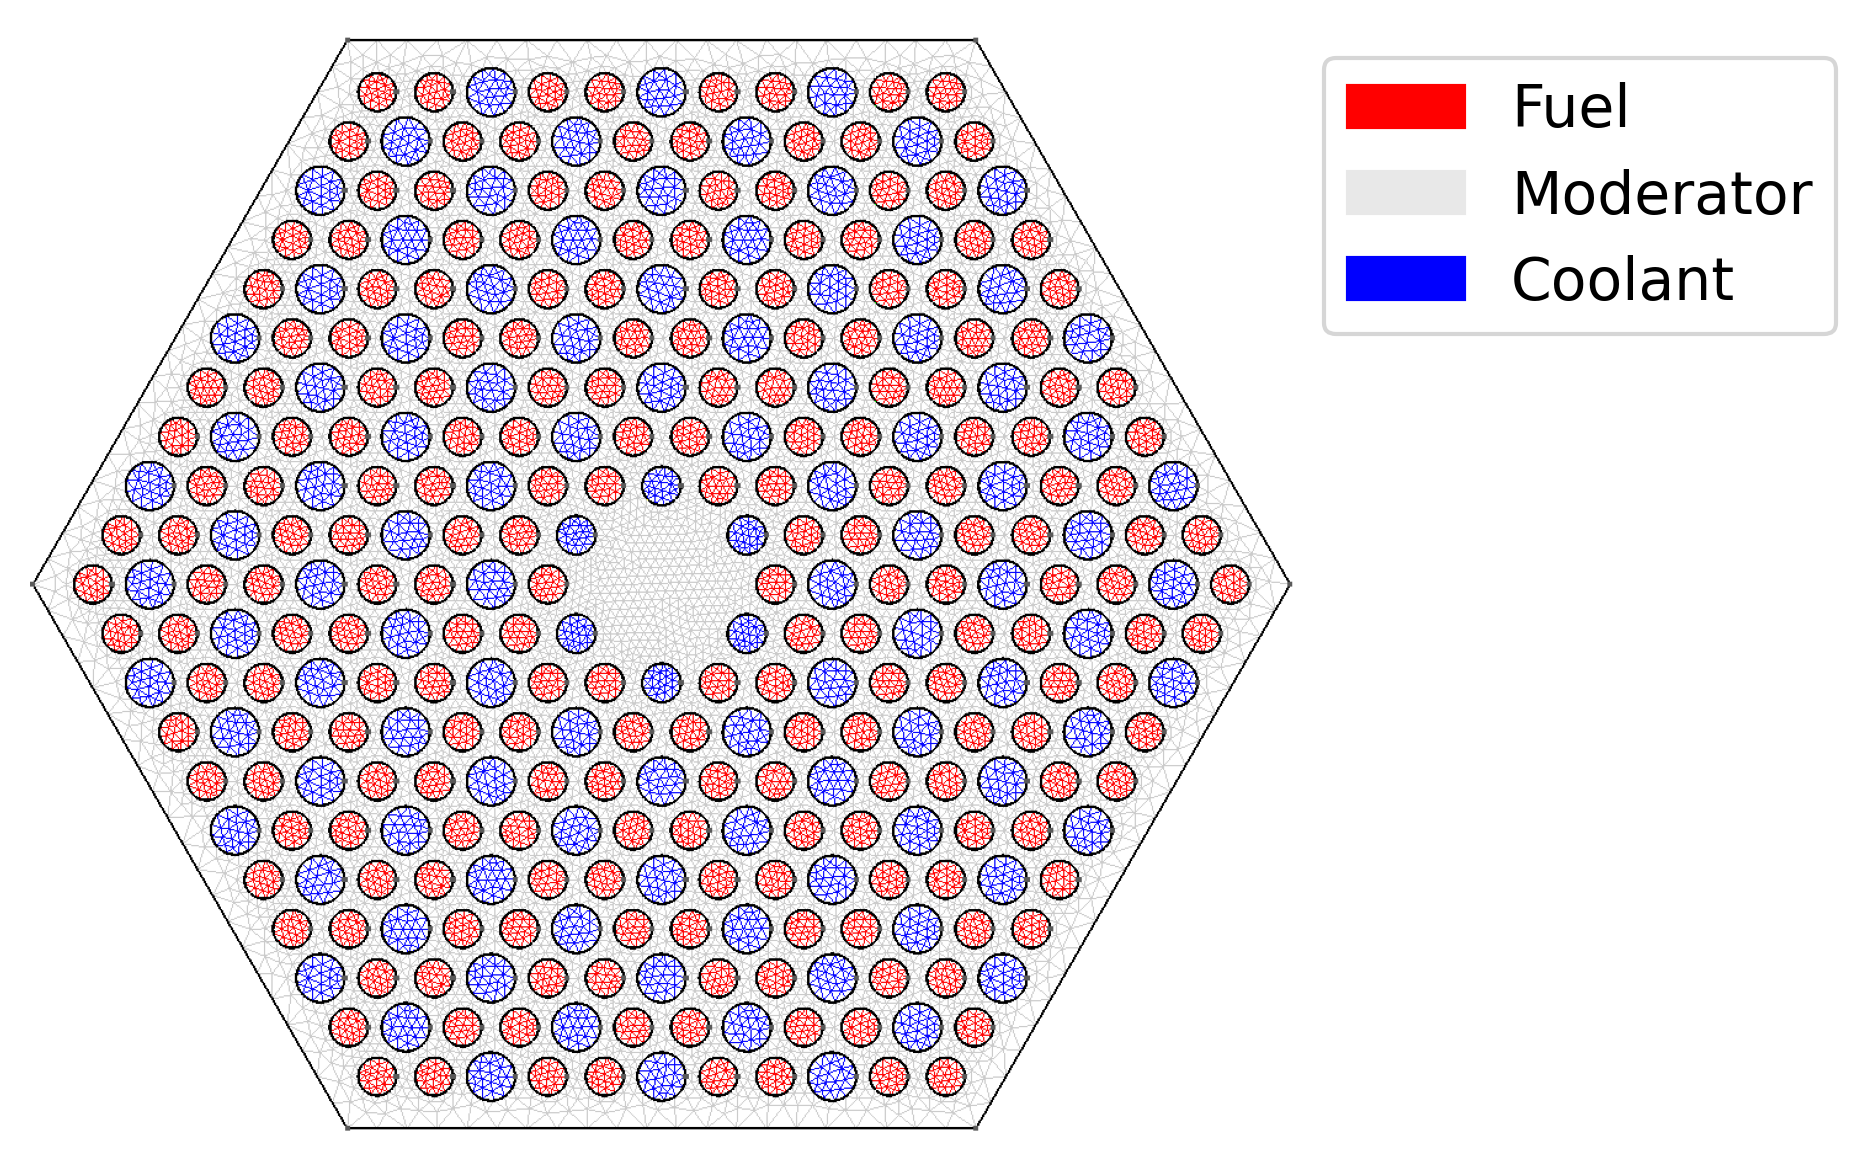
\includegraphics[width=0.45\linewidth]{figures-thermal/full-assem-mesh2}
  \hfill
  \caption{Axial view of the full-fuel column model geometry.}
  \label{fig:th-full-assem-mesh}
\end{figure}

\begin{table}[htbp!]
  \centering
  \caption{Mesh characteristics and maximum temperatures of the full-fuel column model.}
  \label{tab:th-full-assem-results}
\begin{tabular}{lccccc}
\toprule
                            & Mesh 1 & Mesh 2 & Mesh 3 & Mesh 4 & Mesh 5 \\
\midrule
Number of elements [$\times 10^{6}$]  & 1.025 & 1.306 & 1.833 & 2.596 & 3.006 \\
Number of DoFs [$\times 10^{6}$]      & 0.524 & 0.666 & 0.932 & 1.317 & 1.525 \\
Maximum coolant temperature & 1060.41 & 1062.23 & 1064.00 & 1065.13 & 1065.32 \\
Maximum fuel temperature    & 1204.49 & 1217.32 & 1225.57 & 1233.44 & 1234.93 \\
\bottomrule
\end{tabular}
\end{table}

This analysis reveals a potential problem.
The high level of detail in the geometry requires a large number of elements in the mesh.
In the full-scale problem the dimensions and the number of elements in the mesh both increase.
Potentially, this method will be unable to solve the three-dimensional full-scale problem due to a high memory requirement.
For this reason, the next section intends to solve the full-scale problem using a two-dimensional cylindrical model.

% Maybe talk about that the number of nodes in the coolant channels could be reduced as we are using the fluid 1D equations.
% However, the coolant channel mesh requires enough points in the circle to properly model the heat transfer between the solid and the coolant.
% The ideal mesh would have many points in the boundary of the cylinder and one point in the cylinder center.
% But that is not numerically good, as the jacobian of those triangles is too as mall and could cause issues on the simulations.

% \section{Full-core 3D}
% This section will extend the methodology to a full-core problem and it will intend to solve Exercise 2 of Phase I of the OECD/NEA MHTGR-350 Benchmark.

\section{OECD/NEA MHTGR-350 Benchmark: Phase I Exercise 2}
\label{sec:ph1ex2}

This section describes Phase I Exercise 2 of the OECD/NEA MHTGR-350 Benchmark \cite{oecd_nea_benchmark_2017} and the undertaking as part of this thesis to conduct it using Moltres.
Phase I Exercise 2 defines a thermal-fluid stand-alone calculation.
The exercise aims to ensure that the thermal-fluid model differences between participants are negligible and will not affect the coupled exercises.
The benchmark specifies the power density of each fuel region and defines the type of mass flow distribution and material properties for four sub-cases:
\begin{itemize}
  \item Exercise 2a: No bypass flow and fixed thermo-physical properties. The model does not account for the bypass flow, and the thermo-physical properties are constant.
  \item Exercise 2b: Bypass flow type I and fixed thermo-physical properties. This exercise prescribes the bypass flow distribution, and the thermo-physical properties are constant.
  \item Exercise 2c: Bypass flow type I and variable thermo-physical properties. This exercise prescribes the bypass flow distribution and the thermo-physical properties depend on different simulation parameters.
  \item Exercise 2d: Bypass flow type II and variable thermo-physical properties. This exercise solves the bypass flow distribution through the explicit modeling of the bypass gaps. The thermo-physical properties depend on different simulation parameters.
\end{itemize}

The exercise requires reporting the average and maximum temperature values of the reflector, \gls{RPV}, fuel, moderator, and coolant.
It also requires reporting the RPV heat flux and the mass flow rate distribution in the coolant channels and the bypass gaps.
These data are helpful to trace the source of possible differences in the primary parameters between participants.
Since OECD/NEA did not publish the results for this exercise, this section compares Moltres/MOOSE results against INL's benchmark results \cite{strydom_inl_2013}.
This section presents only a subset of available data that illustrate the main characteristics of the exercise.

Figure \ref{fig:ex2a-1st-model} displays the model geometry.
The model uses several simplifications to conduct the exercise.
In the axial direction, it does not consider the upper plenum and the outlet plenum, and the axial boundaries are the top reflector's upper face and the bottom reflector's lower face.
The top reflector's upper face and the inlet coolant flow are at 259 $^{\circ}$C, while the bottom reflector's lower face is adiabatic.
The outlet coolant uses an outflow boundary condition.
In the radial direction, the model does not consider the core barrel and the helium gap.
The model includes the RPV, followed by the outside air.
The outside air region outer boundary is at 30 $^{\circ}$C.

% model H figure
\begin{figure}[htbp!]
  \centering
  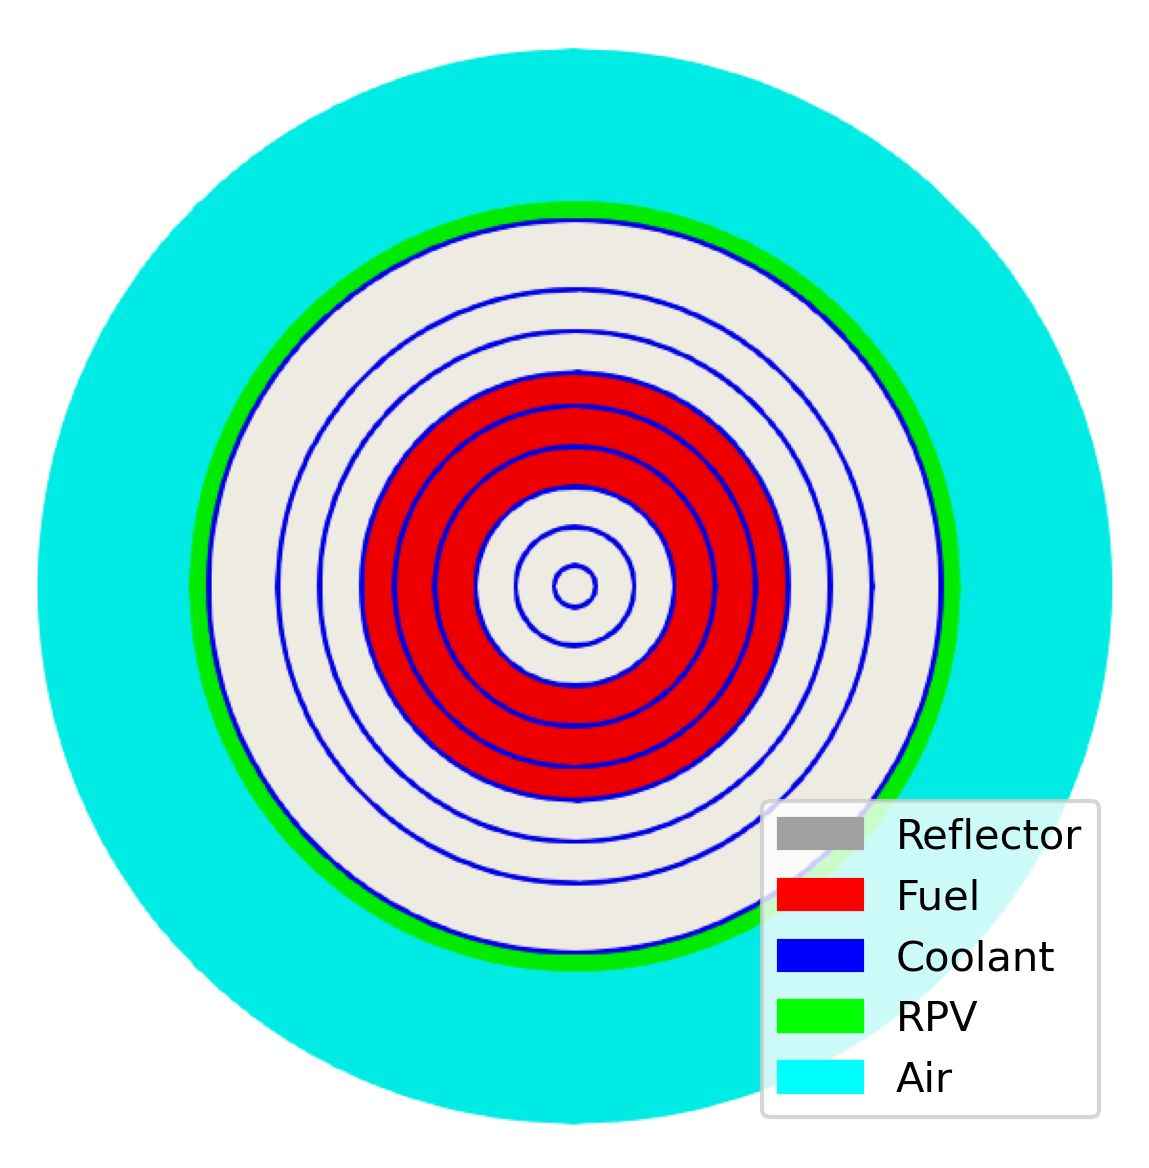
\includegraphics[width=0.45\linewidth]{figures-thermal/ex2a-meshD2}
  \hfill
  \caption{Phase I Exercise 2 model geometry for simulation in Moltres.}
  \label{fig:ex2a-1st-model}
\end{figure}

The core model geometry uses INL's model as the reference design.
Nine rings define the solid structures in the core, and the other nine rings the coolant flow in the core.
I calculated the radii of the rings by preserving the assemblies' volume.
The coolant thickness is constant for all the rings and preserves the coolant volume in the core.
% missing description of the power density distribution
Table \ref{tab:th-ex2a} presents the material properties.
All the graphite regions assume the grade H-451 graphite material properties.

\begin{table}[htbp!]
\centering
      \caption{Problem characteristics.}
      \label{tab:th-ex2a}
      % \begin{tabular}{@{}l S[table-format=3.5] c c}
      \begin{tabular}{@{}l c c c}
    \toprule
  \multicolumn{1}{c}{Parameter} & \multicolumn{1}{c@{}}{Value} & \multicolumn{1}{c@{}}{Units} & \multicolumn{1}{c}{Reference} \\    
    \midrule
  Fuel compact thermal conductivity & 20    & W $\cdot m^{-1} \cdot K^{-1}$ & \cite{oecd_nea_benchmark_2017} \\
  Fuel block thermal conductivity   & 37    & W $\cdot m^{-1} \cdot K^{-1}$ & \cite{oecd_nea_benchmark_2017} \\
  Graphite thermal conductivity     & 66    & W $\cdot m^{-1} \cdot K^{-1}$ & \cite{oecd_nea_benchmark_2017} \\
  \gls{RPV} thermal conductivity    & 40    & W $\cdot m^{-1} \cdot K^{-1}$ & \cite{oecd_nea_benchmark_2017} \\
  Coolant thermal conductivity      & 0.41  & W $\cdot m^{-1} \cdot K^{-1}$ & \cite{oecd_nea_benchmark_2017} \\
  Air thermal conductivity          & 0.068 & W $\cdot m^{-1} \cdot K^{-1}$ & \cite{oecd_nea_benchmark_2017} \\
  Helium density                    & 5.703 & $\times 10^{-6}$ kg $\cdot cm^{-3}$  & \cite{nist_thermophysical_2020} \\
  Helium heat capacity              & 5188  & J $\cdot kg^{-1} \cdot K^{-1}$  & \cite{nist_thermophysical_2020} \\
  \bottomrule
  \end{tabular}
\end{table}

Table \ref{tab:th-ex2a-1st-results} displays the results.
The model considerably under-predicts the inner reflector rings temperature, while it over-predicts the coolant rings temperature.
With the purpose of better understanding this behavior, Figure \ref{fig:ex2a-1st-model-across} shows the temperature across the reactor on the bottom of the active core (z=200 cm).
This figure exposes that the temperatures in the active core are well above the other region temperatures.
Although such behavior is expected, the temperature profile reveals some heat transfer disconnection between the different rings.
In other words, the heat transfer from the fuel rings to the rest of the core structures is smaller than the heat transfer to the coolant rings in the active core region.
This thermal disconnection causes the reflector temperatures to be too low and the coolant temperatures in the fuel rings too high.
These results indicate that Moltres model fails to capture some heat transfer mechanisms that INL's model captures.
The most obvious difference between the models is the inclusion of the radiative heat transfer.
Future Moltres development efforts will focus on confirming this supposition and adding the capability to model the radiative heat transfer.

\begin{table}[htbp!]
\centering
      \caption{Comparison of this work and INL \cite{strydom_inl_2013} first bottom core level average temperatures.}
      \label{tab:th-ex2a-1st-results}
\begin{tabular}{lcccccc}
    \toprule
                & \multicolumn{3}{c}{Reflector} & \multicolumn{3}{c}{Coolant}   \\
                & Ring 1   & Ring 2   & Ring 3   & Ring 4   & Ring 5  & Ring 6  \\
    \midrule
INL [$^{\circ}C$]           & 790    & 794     & 802     & 797     & 636     & 673     \\
Moltres/MOOSE [$^{\circ}C$] & 268    & 313     & 769     & 1424    & 1597    & 1157    \\
$\Delta_T$ [\%]    & 66       & 61     & 4       & 79      & 151     & 72      \\
    \bottomrule
  \end{tabular}
\end{table}

\begin{figure}[htbp!]
  \centering
  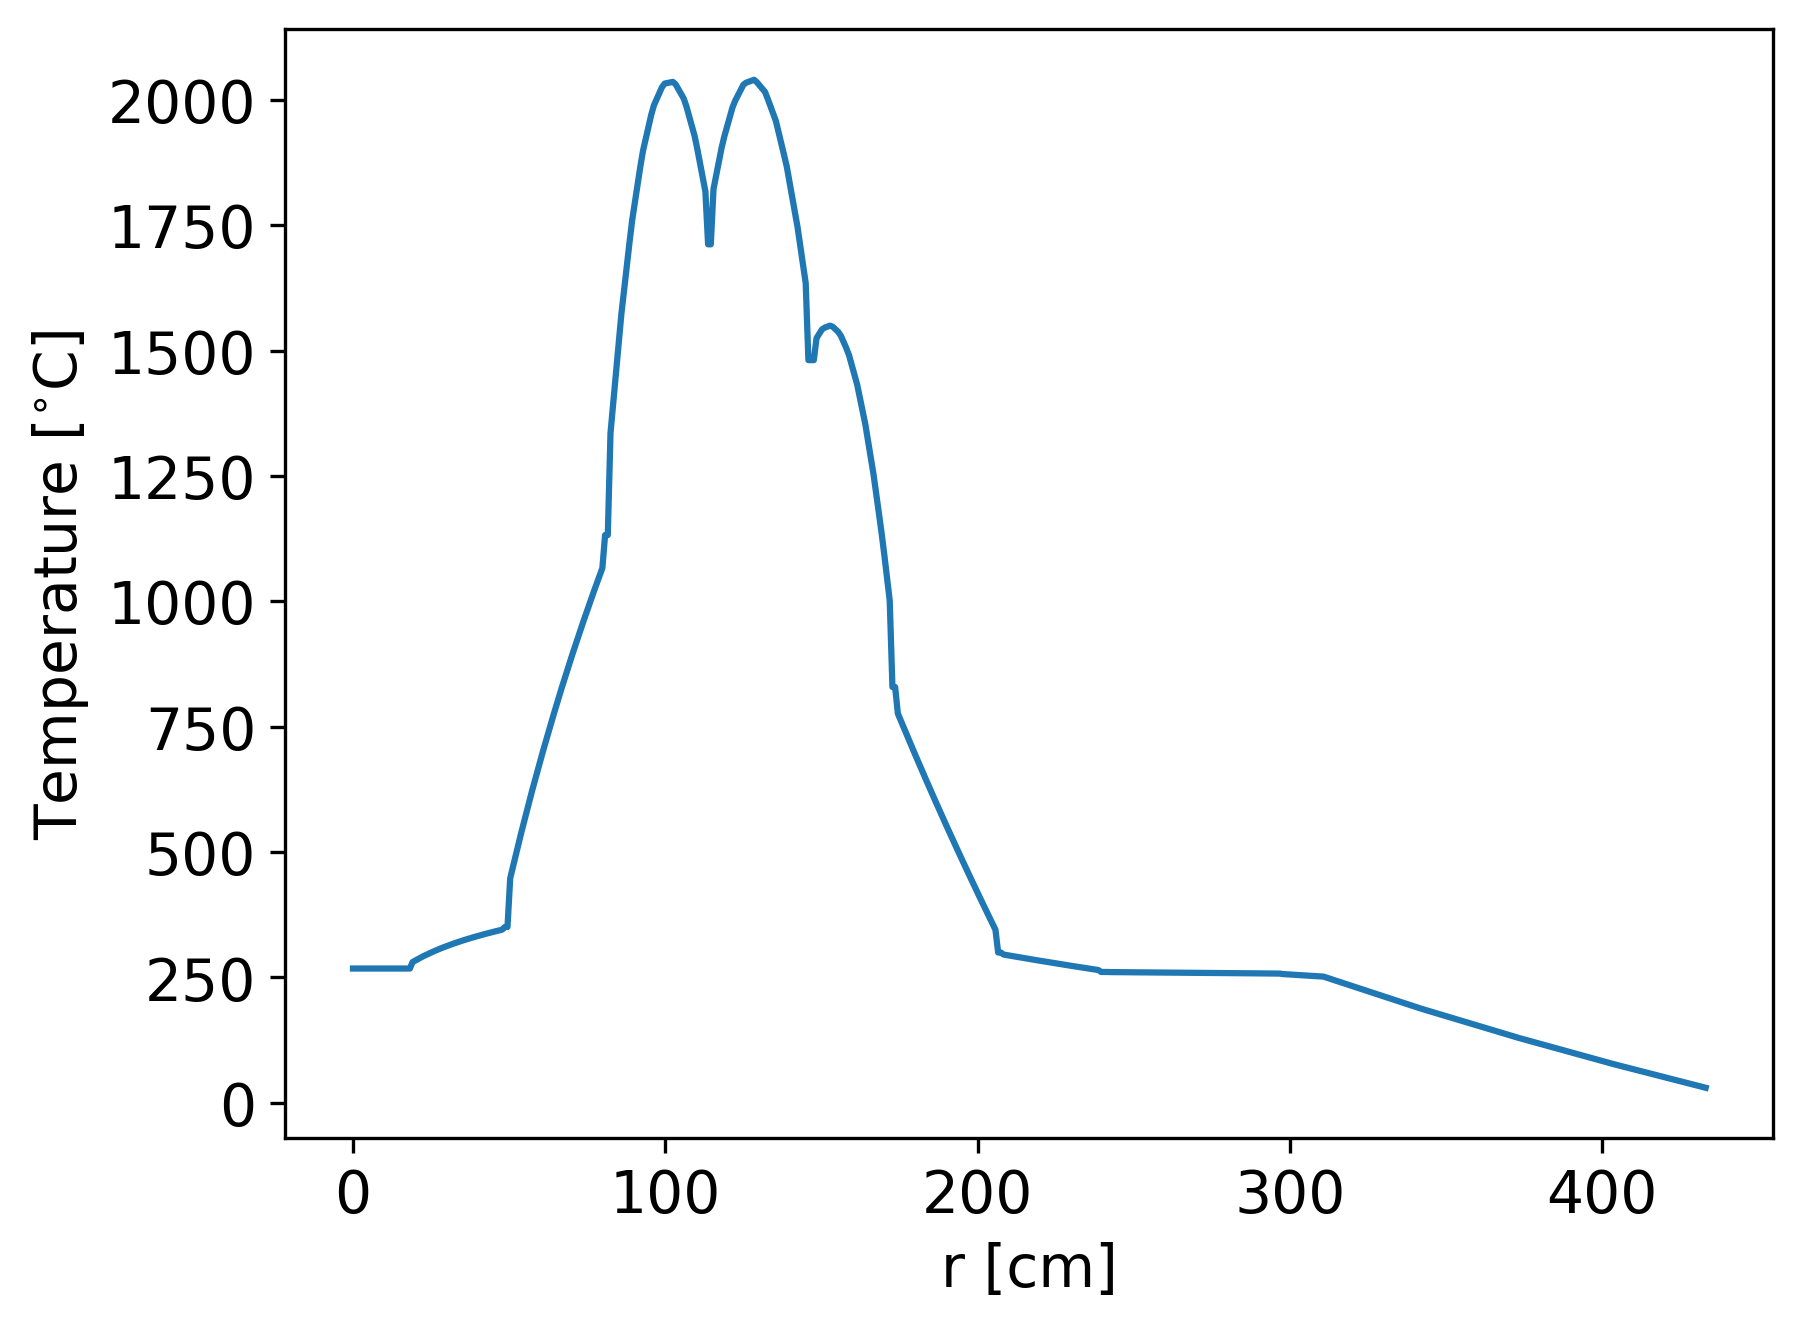
\includegraphics[width=0.45\linewidth]{figures-thermal/ex2a-across}
  \hfill
  \caption{Radial temperature at the bottom of the active core (z=200 cm) determined by Moltres.}
  \label{fig:ex2a-1st-model-across}
\end{figure}

% left here on review
To circumvent this barrier, the following analysis considered a second model based on Stainsby's approach \cite{stainsby_investigation_2008}.
% which defines only one coolant ring for each fuel ring.
The calculation used a global model to obtain the coolant temperature in the core and then a sub-channel model to get the fuel and moderator average temperatures.
The sub-channel model used half of the unit cell from Section \ref{sec:unitcell}.
Figure \ref{fig:ex2a-2nd-model} displays the global model geometry.
Three fuel rings represent the three rings of fuel assemblies in the MHTGR-350 (see Figure \ref{fig:layout}).
In the middle of each fuel ring, a coolant ring defines the coolant flow in that fuel ring.
The radii of the rings preserves the assemblies' volume, and the coolant ring volumes preserve the coolant volume in each of the fuel rings.
The model uses the material properties from Table \ref{tab:th-ex2a}.

Figure \ref{fig:ex2a-temps} presents the coolant and solid temperatures in the different fuel rings.
The coolant temperature increases from the top to the bottom of the active core, and it is constant in the bottom and top reflector regions.
The highest coolant, fuel, and moderator temperatures are in Fuel Ring 1.

Table \ref{tab:th-ex2a-results} compares Moltres/MOOSE results to INL's \cite{strydom_inl_2013}.
For the coolant temperature, Moltres results are 9.9\% smaller in Fuel Ring 1, and 1.6 and 3.4\% higher in Fuel Rings 2 and 3.
Although the discrepancies are small, for some reason, the global model fails to correctly distribute the heat produced in the fuel rings into the coolant rings.
A possible cause of this discrepancy is the flat velocity approximation.
Section \ref{sec:flowdistrib} showed that a flat velocity distribution of the coolant is reasonable in the fuel column model; however, one of the assumptions of that model was a uniform power density.
In this exercise, the power density is not uniform, which could explain the discrepancies.
Further studies might confirm their cause.

Additionally, Moltres predicts a smaller coolant-to-moderator temperature difference for Fuel Rings 1 and 2.
The most considerable discrepancy is in Fuel Ring 1.
INL's model coolant-to-moderator temperature difference is 46$^{\circ}$C while Moltres/MOOSE predicts a difference of 30$^{\circ}$C.
The flat velocity approximation might be again the source of these discrepancies.
Finally, the moderator-to-fuel temperature differences from INL and Moltres/MOOSE are close.
In Fuel Ring 1, the differences are 20$^{\circ}$C and 22$^{\circ}$C for INL and Moltres/MOOSE results, respectively.
In fuel ring 2, the differences are 16$^{\circ}$C and 17$^{\circ}$C for INL and Moltres/MOOSE results.

% model G figure
\begin{figure}[htbp!]
  \centering
  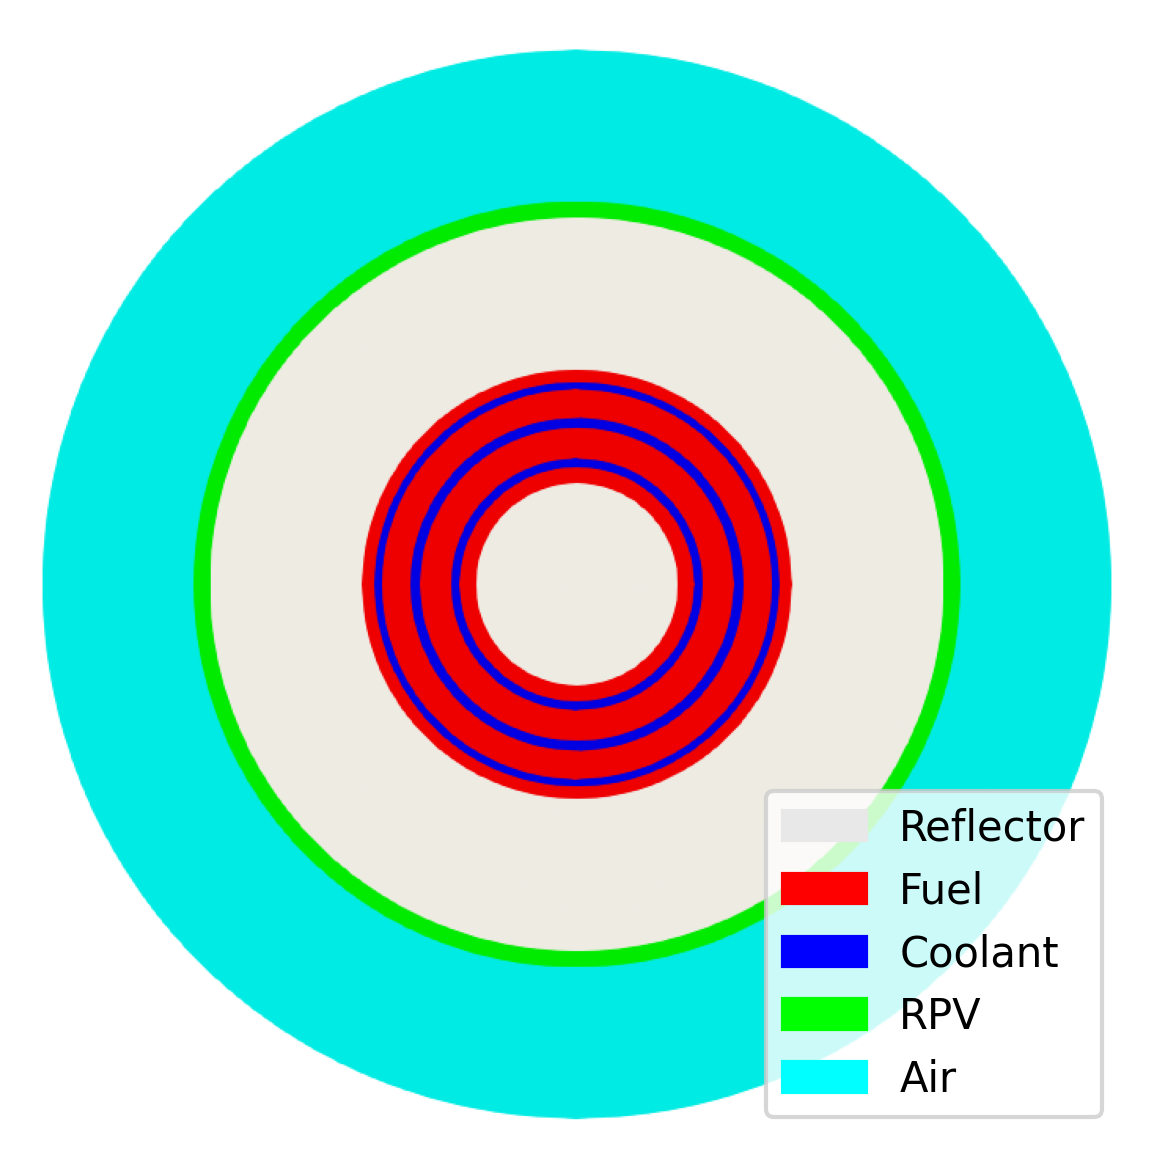
\includegraphics[width=0.4\linewidth]{figures-thermal/ex2a-meshC2}
  \hfill
  \caption{Model geometry.}
  \label{fig:ex2a-2nd-model}
\end{figure}

% model G results
\begin{figure}[htbp!]
  \centering
    \subfloat[Coolant temperature in the different fuel rings.]{
        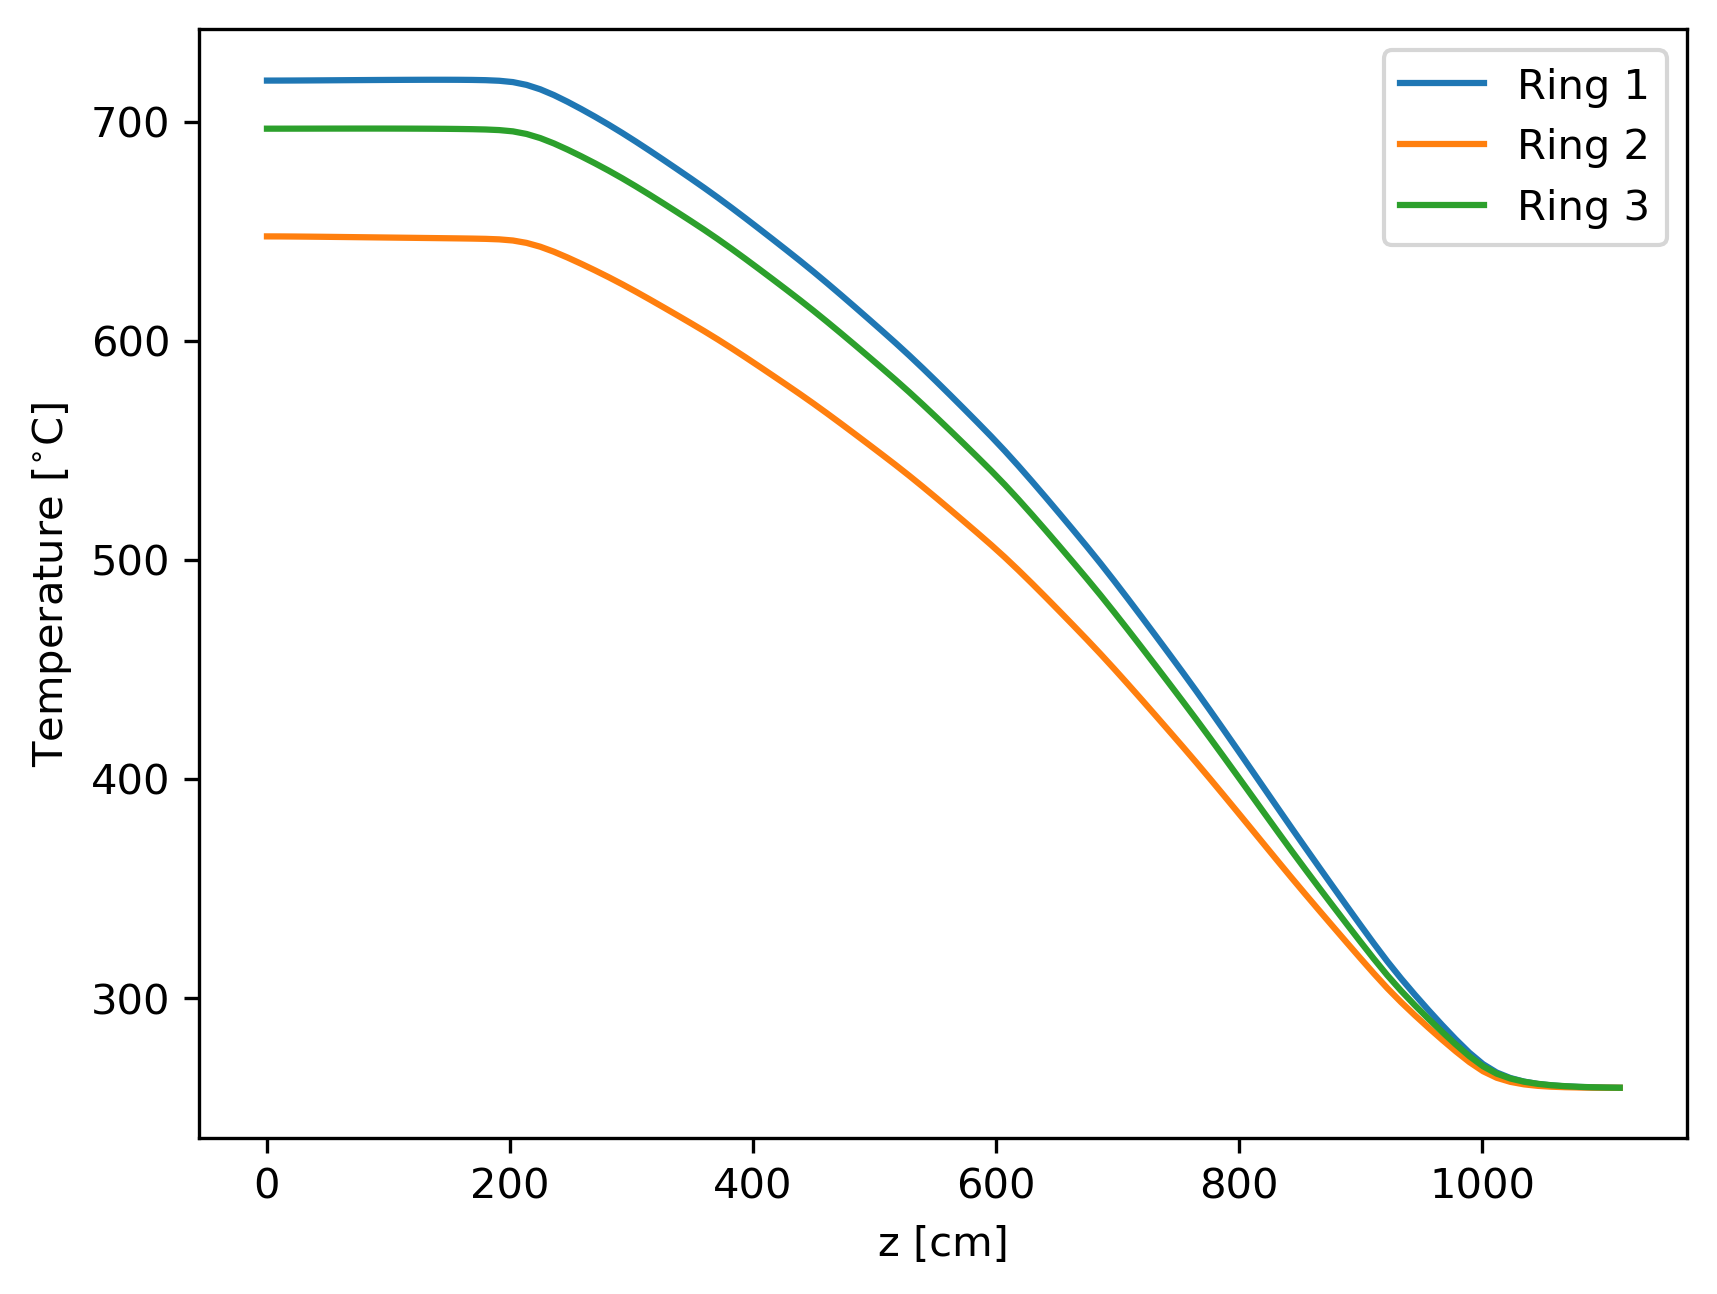
\includegraphics[width=0.45\textwidth]{figures-thermal/ex2a-fullcore-cool}
    }
    \subfloat[Average moderator and fuel temperatures in the different fuel rings.]{
        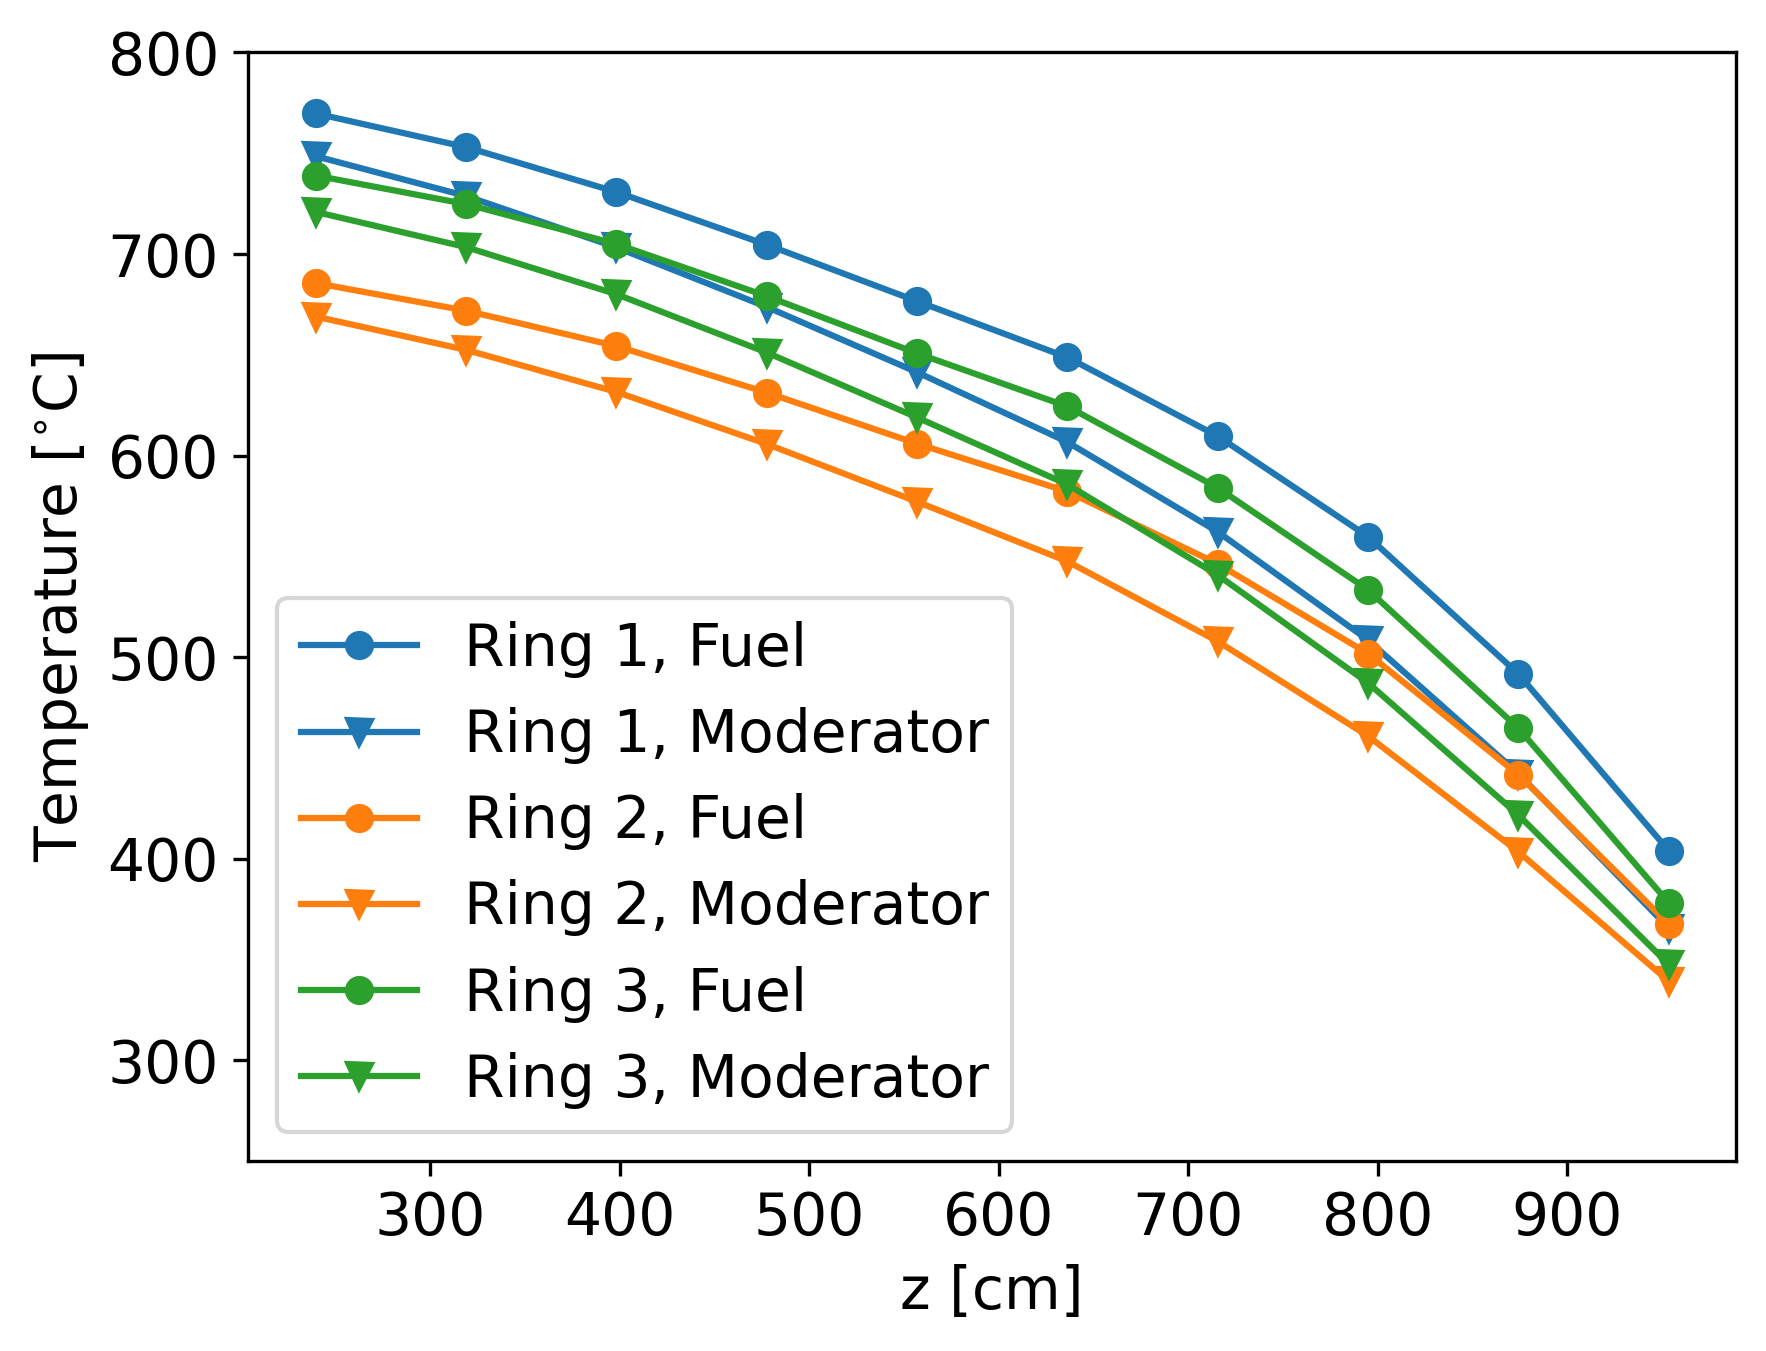
\includegraphics[width=0.45\textwidth]{figures-thermal/ex2a-solid}
    }
  \hfill
  \caption{Axial temperatures determined by Moltres.}
  \label{fig:ex2a-temps}
\end{figure}

\begin{table}[htbp!]
\centering
      \caption{Comparison of this work and INL \cite{strydom_inl_2013} first bottom core level average temperatures. Temperature values expressed in [$^{\circ}$C].}
      \label{tab:th-ex2a-results}
  \begin{tabular}{l|ccc|ccc|ccc}
    \toprule
          & \multicolumn{3}{c|}{Fuel Ring 1} & \multicolumn{3}{c|}{Fuel Ring 2} & \multicolumn{3}{c}{Fuel Ring 3} \\ %\cline{2-10} 
          & Coolant & Moderator & Fuel & Coolant & Moderator & Fuel & Coolant & Moderator & Fuel \\
    \midrule
INL          & 797  & 843  & 863  & 636  & 672  & 688  & 673  & Not shown  & 722  \\
This thesis  & 718  & 748  & 770  & 646  & 669  & 686  & 696  & 721        & 739  \\
$\Delta_T$ [\%]     & 9.9  & 11.3 & 10.8 & 1.6  & 0.4  & 0.3  & 3.4  & -  & 2.4  \\
    \bottomrule
  \end{tabular}
\end{table}

\section{Coupled simulations}
\label{sec:thermal-coupling}

This section sets the roadmap for conducting neutronics and thermal-fluids coupled simulations of prismatic HTGRs in Moltres.

\subsection{OECD/NEA MHTGR-350 Benchmark: Phase I Exercise 3}
\label{sec:ph1ex3}

% description of the exercise
This section presents Phase I Exercise 3 of the OECD/NEA MHTGR-350 Benchmark and describes the exercise conducted with Moltres/MOOSE.
Exercise 3 combines all the data from the first two exercises of the benchmark, in which the participants need to determine a coupled neutronic and thermal-fluids solution.
The exercise requires the reporting of the same parameters reported in Exercises 1 and 2 combined.
The benchmark specifies the group constants necessary to conduct the exercise.
The group constants depend on four state parameters: moderator ($T_m$) and fuel temperature ($T_f$) and xenon-135 ($C_{Xe}$) and hydrogen concentration ($C_H$).
In addition to these data, the benchmark provides fluence maps to determine the thermal conductivity of graphite.

Two sub-cases compose Exercise 3:
\begin{itemize}
  \item Exercise 3a: Same thermal-fluids problem definition from Exercise 2c. This exercise prescribes the bypass flow distribution and the thermo-physical properties depend on the temperature and fluence.
  \item Exercise 3b: Same thermal-fluids problem definition from Exercise 2d. This exercise solves the bypass flow distribution through the explicit modeling of the bypass gaps. The thermo-physical properties depend on depend on the temperature and fluence.
\end{itemize}

% initial coupling: description of what I've done
Section \ref{sec:ph1ex2} solved the thermal-fluids stand-alone problem using a global and a sub-channel model.
Those simulations required running two separate input files, where the output of the global model served as an input to the sub-channel model.
Exercise 3 requires modeling the temperature feedback.
Using Section \ref{sec:ph1ex2} approach for the temperature feedback would require the fully-coupled simulation of both input files.
However, MOOSE framework did not have the capability to couple these specific input files at the moment of carrying out this exercise.

To solve Exercise 3, I used a simplified global model, requiring the simulation of only one input file.
The global model homogenizes the fuel and moderator materials.
The explicit modeling of the fuel in the global model requires the conversion of the fuel dimensions in the three-dimensional geometry to the simplified cylindrical model.
This conversion requires the conservation of two parameters, the fuel volume and the fuel thickness.
The fuel volume ensures that the reactor power does not change in the approximation.
The maximum fuel temperature is very sensitive to the fuel thickness, requiring its preservation.
Conserving both parameters simultaneously is not possible, and the global model homogenizes the fuel and moderator materials.
Hence, the solution of this model did not differentiate between moderator and fuel.

% describe the model
Figure \ref{fig:coupled-mesh} presents the model geometry.
The model includes 28 fuel and 29 coolant rings.
I calculated the radii of the rings by preserving the assemblies' and the coolant volume.
The coolant ring pitch is the coolant channel pitch in a fuel assembly.
Exercise 3a requires using material properties from Exercise 2c.
This simplified model used the material properties from Exercise 2a, as shown in Table \ref{tab:th-ex2a}.
Regarding the group-constants, the benchmark prescribes them for 232 regions in the reactor.
Table \ref{tab:coupled-rz} shows what benchmark sub-domains integrate each model region.
The model did not include the control rod region (sub-domain 232).
The simulations used a three energy-group structure.
Table \ref{tab:coupled-eg} indicates what benchmark group numbers integrate each model group.
Conducting this exercise required the development of a Python tool to translate the benchmark group constants to Moltres format.
The tool was responsible for homogenizing and collapsing the group constants as well.
For further detail on the group constants handling refer to Sections \ref{appendix:group-const-homo} to \ref{appendix:group-const-bench}.
The problem assumed the same boundary conditions from Section \ref{sec:ph1ex2}.

Because Moltres can decouple the neutronics from the thermal-fluid effects, and for the sake of comparison, I conducted the exercise with and without thermal feedback.
The calculations without thermal feedback assumed the group constants at 550 $^{\circ}$C.
Figure \ref{fig:coupled-results-flux} and \ref{fig:coupled-results-th} display the results on two arbitrarily located lines across the core, axial line on $r=85 cm$ and radial line on $z=556.5 cm$.
The thermal feedback affects the flux, which consequently affects the thermal-fluids.
The axial flux peak moves towards the reactor top, where the temperatures are lower than the bottom.
Thus, the heat production shifts towards the reactor top, and the temperatures near the reactor outlet decrease.
The radial temperature profile has a similar shape to the thermal flux, as this group is the main contributor to fission and thus the power profile.
The radial flux does not change considerably, hence the temperature profile does not change much either.
The thermal feedback moves the radial temperature profile up because the heat production shifts towards the top.

\begin{figure}[htbp!]
  \centering
  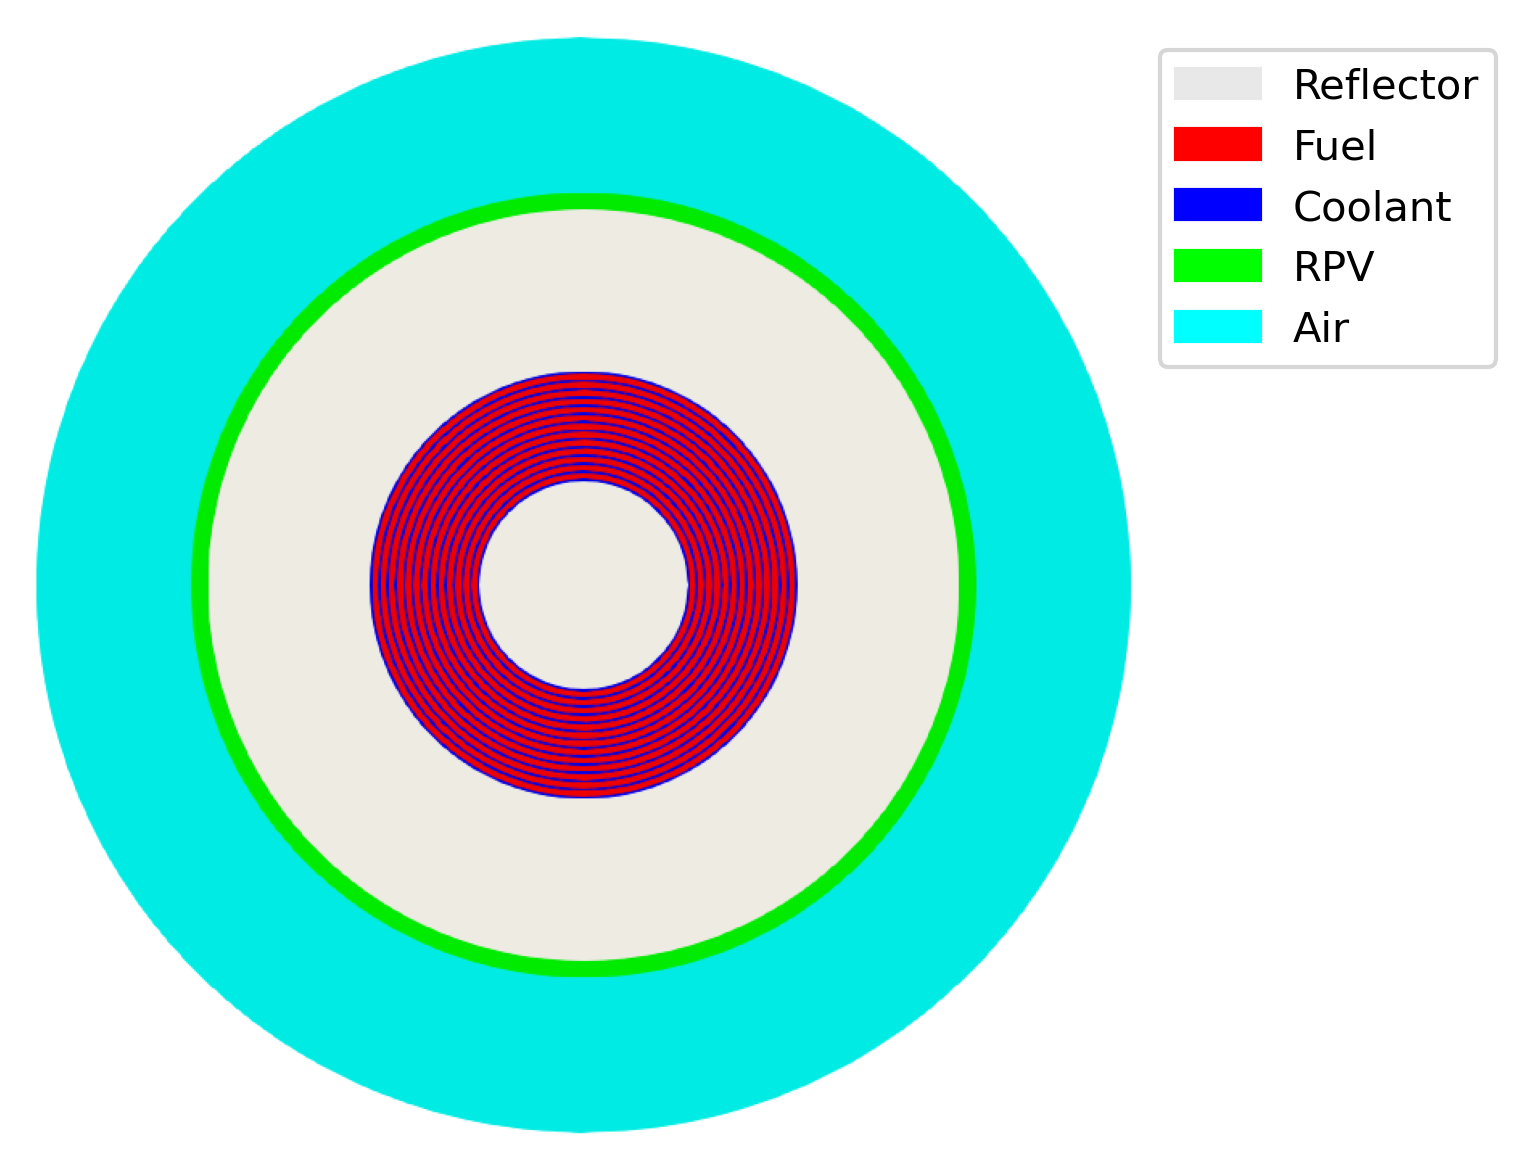
\includegraphics[width=0.45\linewidth]{figures-thermal/ex3-mesh}
  \hfill
  \caption{Axial view of the model geometry.}
  \label{fig:coupled-mesh}
\end{figure}

\begin{table}[htbp!]
\centering
      \caption{Homogenization scheme.}
      \label{tab:coupled-rz}
    \begin{tabular}{l c}
  \toprule
  Model homogenized region & Benchmark sub-domains \\
  \midrule
  Fuel               & 1-220   \\
  Bottom reflector   & 221-224 \\
  Top reflector      & 228-231 \\
  Inner reflector    & 225     \\
  Outer reflector    & 226-227 \\
  \bottomrule
  \end{tabular}
\end{table}

\begin{table}[htbp!]
\centering
      \caption{Energy group condensation scheme.}
      \label{tab:coupled-eg}
    \begin{tabular}{c c}
  \toprule
  Model group number & Benchmark group number \\
  \midrule
  1 & 1-4   \\
  2 & 5-15  \\
  3 & 16-26 \\
  \bottomrule
  \end{tabular}
\end{table}

\begin{figure}[htbp!]
  \centering
    \subfloat[Axial flux over the line at r=85 cm.]{
        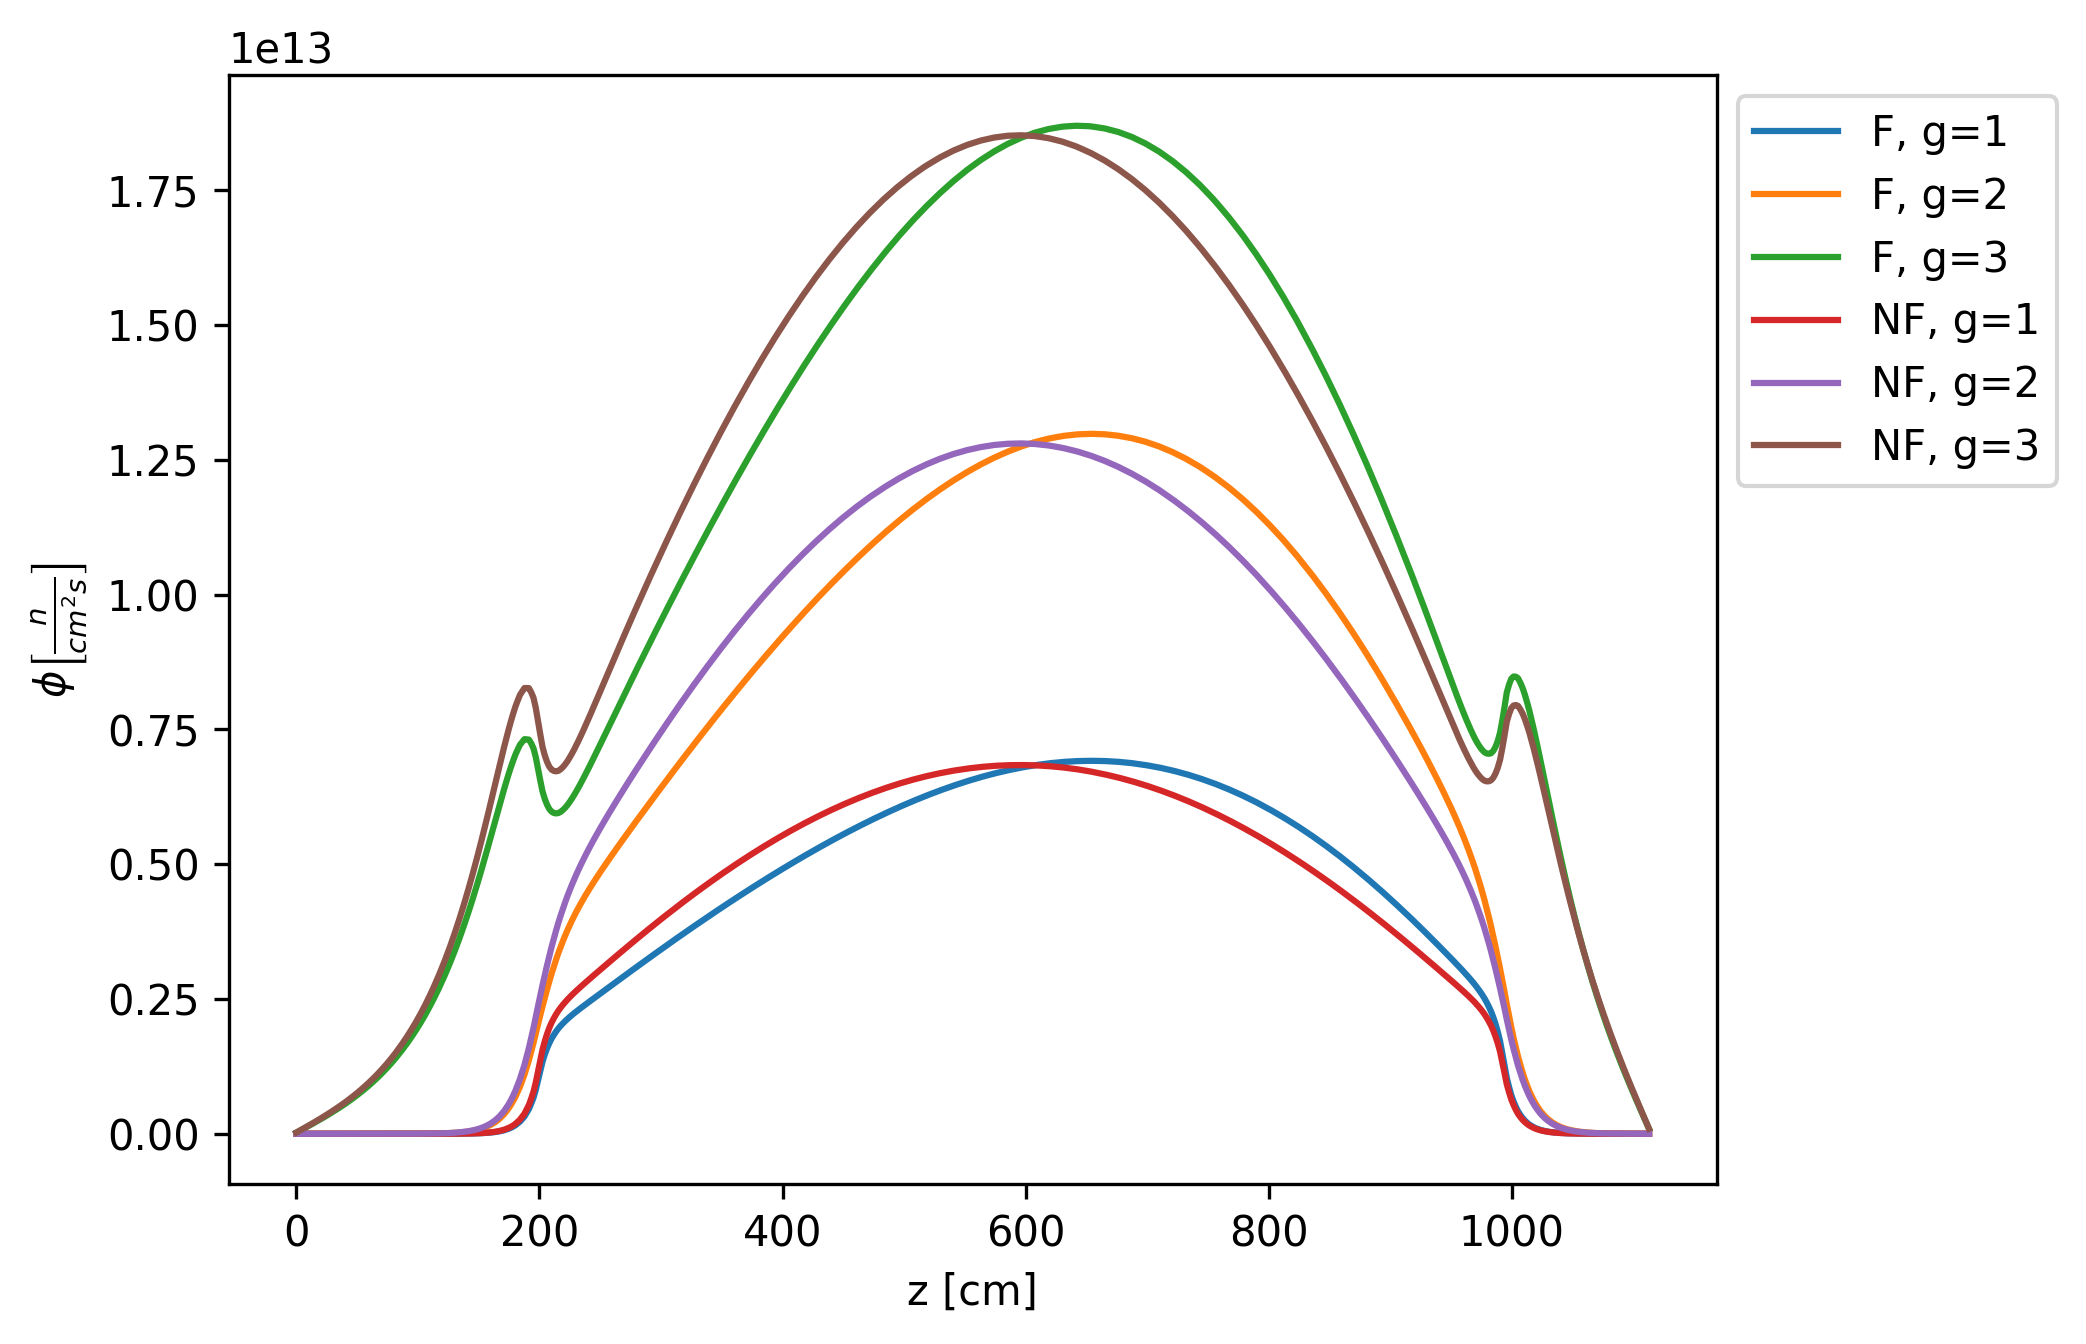
\includegraphics[width=0.45\textwidth]{figures-thermal/coupledD-3G-axial}
    }
    \subfloat[Radial temperature at z=L/2=556.5 cm]{
        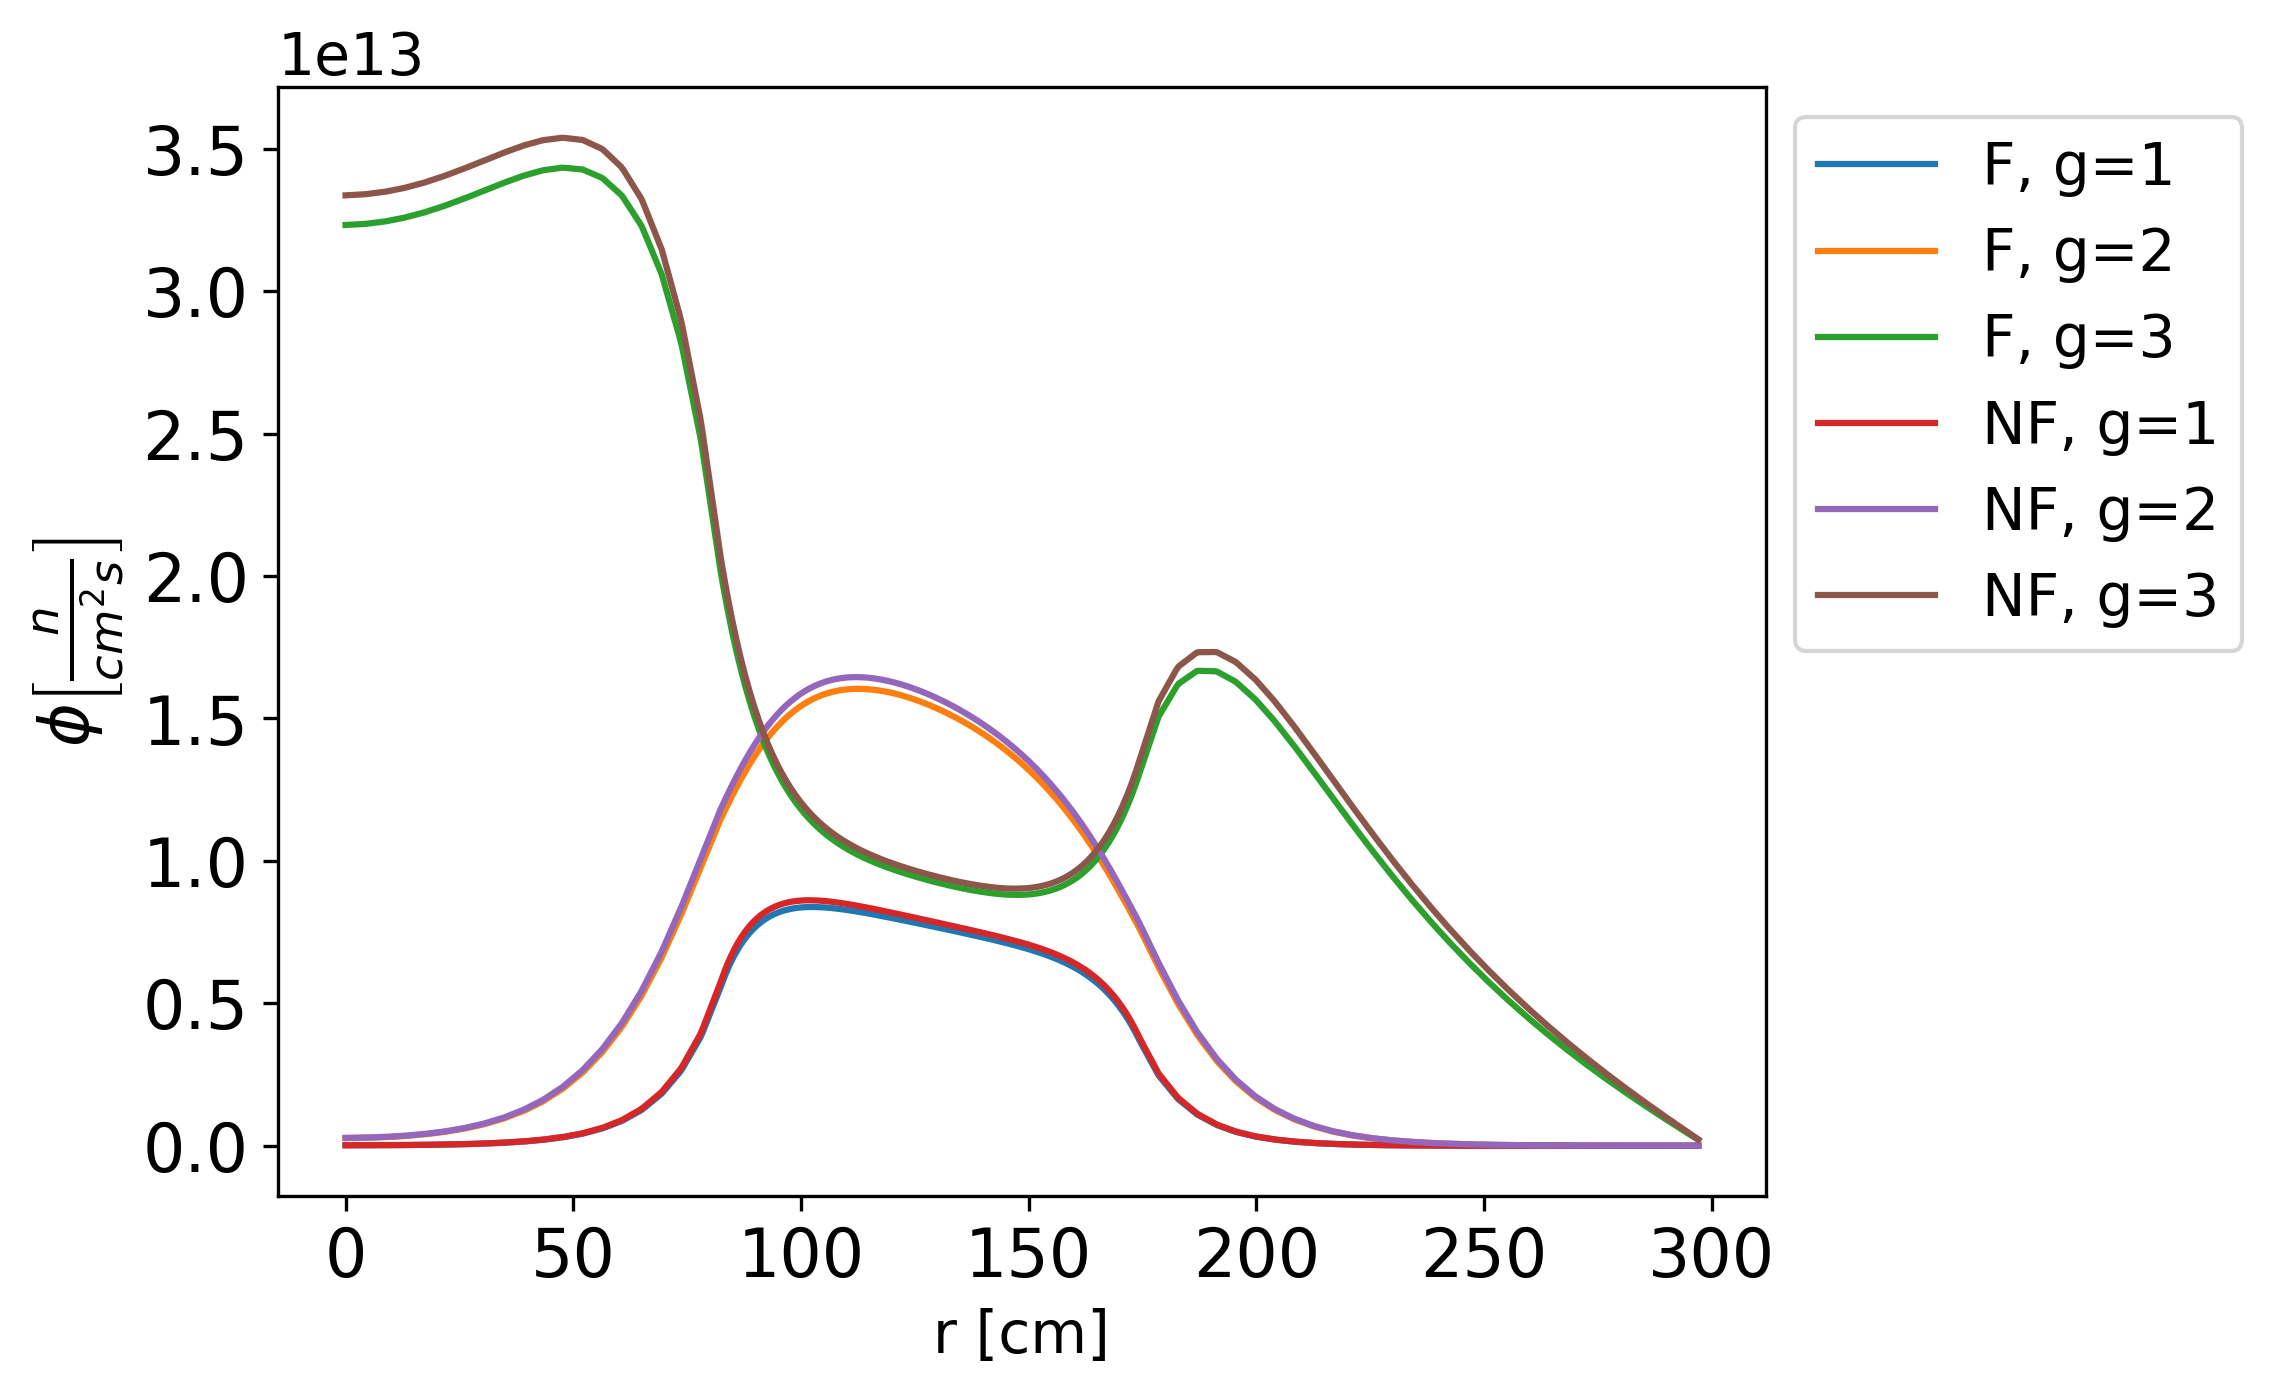
\includegraphics[width=0.45\textwidth]{figures-thermal/coupledD-3G-radial}
    }
  \hfill
  \caption{Flux profile comparison. F: thermal feedback, NF: no thermal feedback.}
  \label{fig:coupled-results-flux}
\end{figure}

\begin{figure}[htbp!]
  \centering
    \subfloat[Axial temperature at r=85 cm.]{
        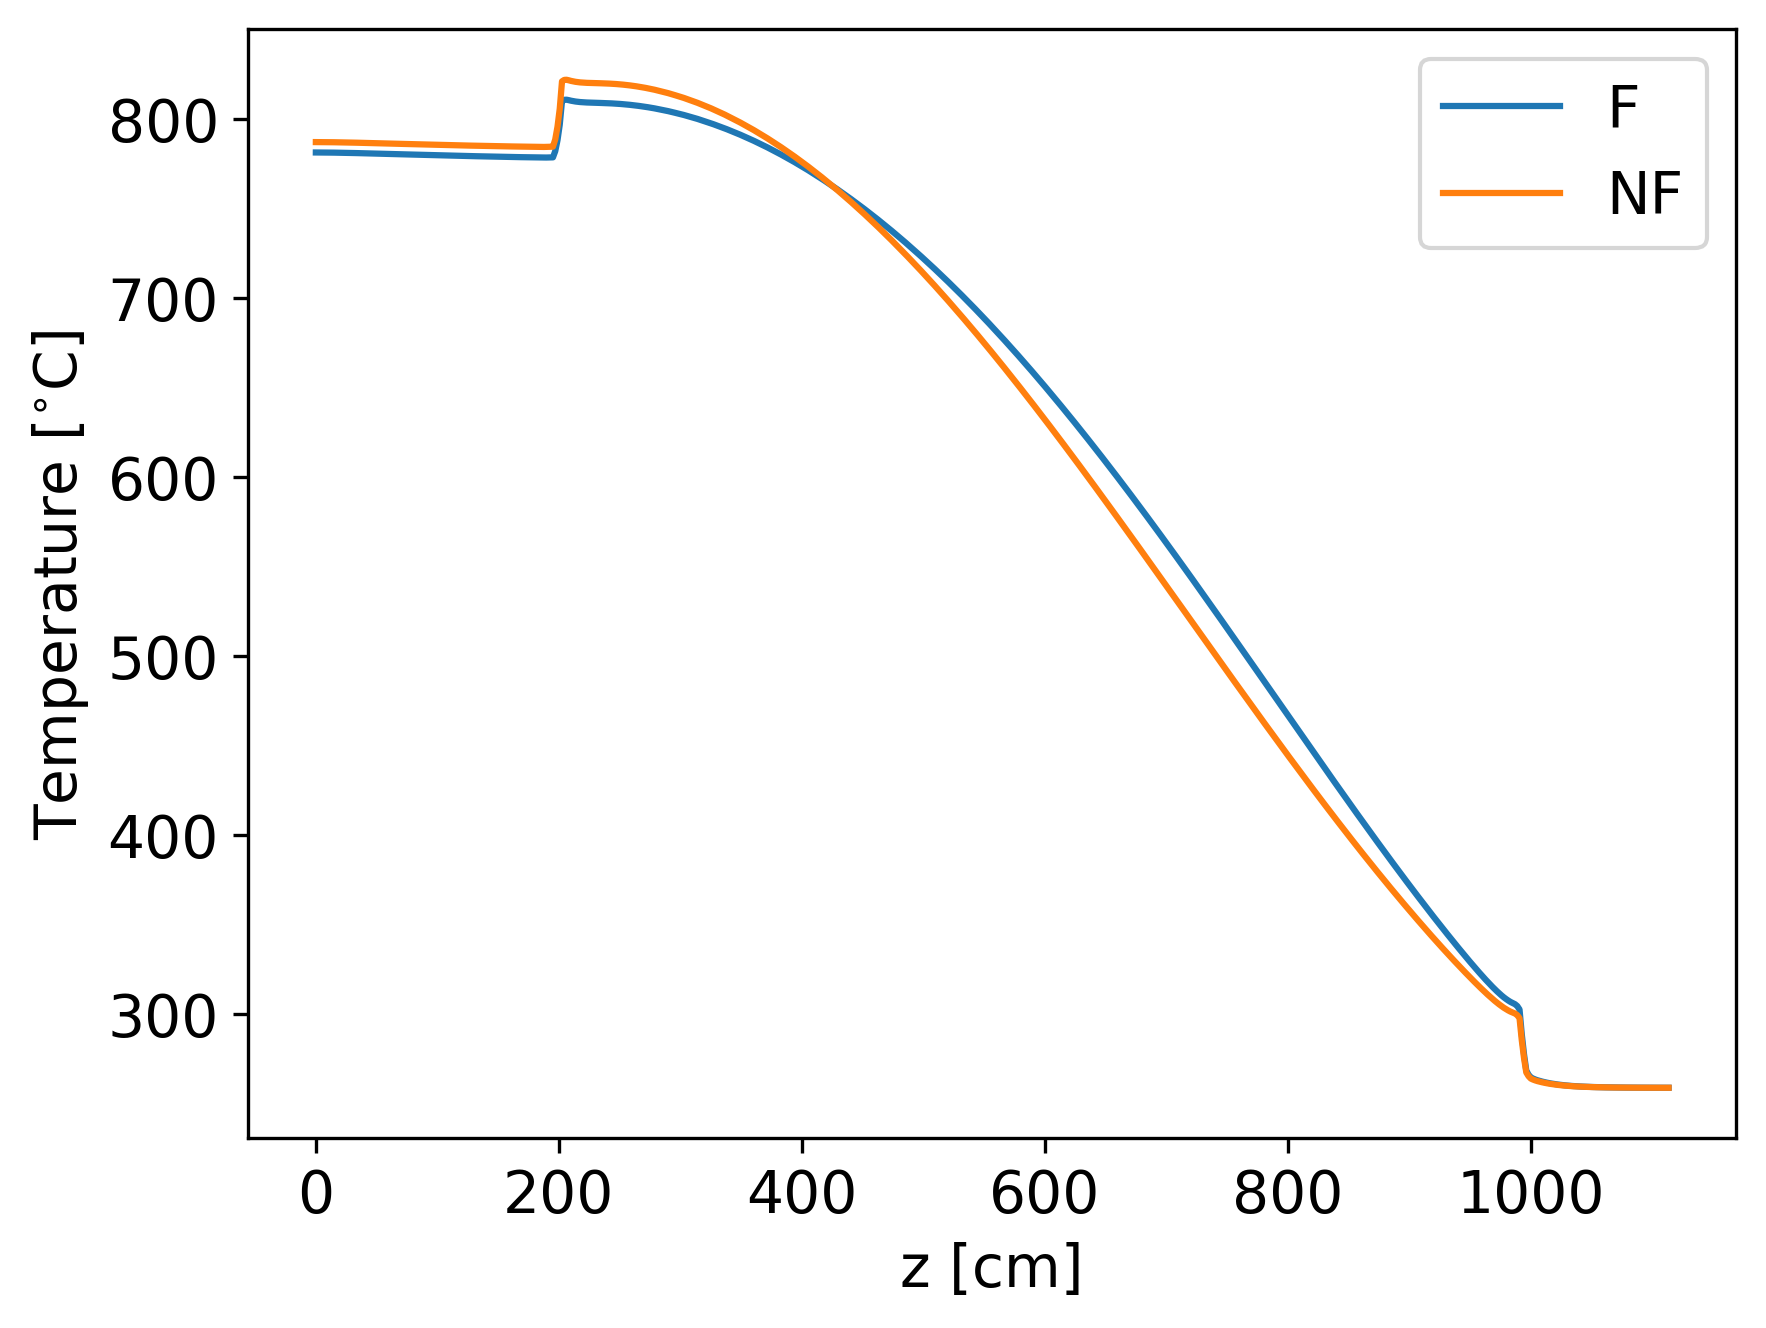
\includegraphics[width=0.45\textwidth]{figures-thermal/coupledD-3G-axialT}
    }
    \subfloat[Radial temperature at z=L/2=556.5 cm]{
        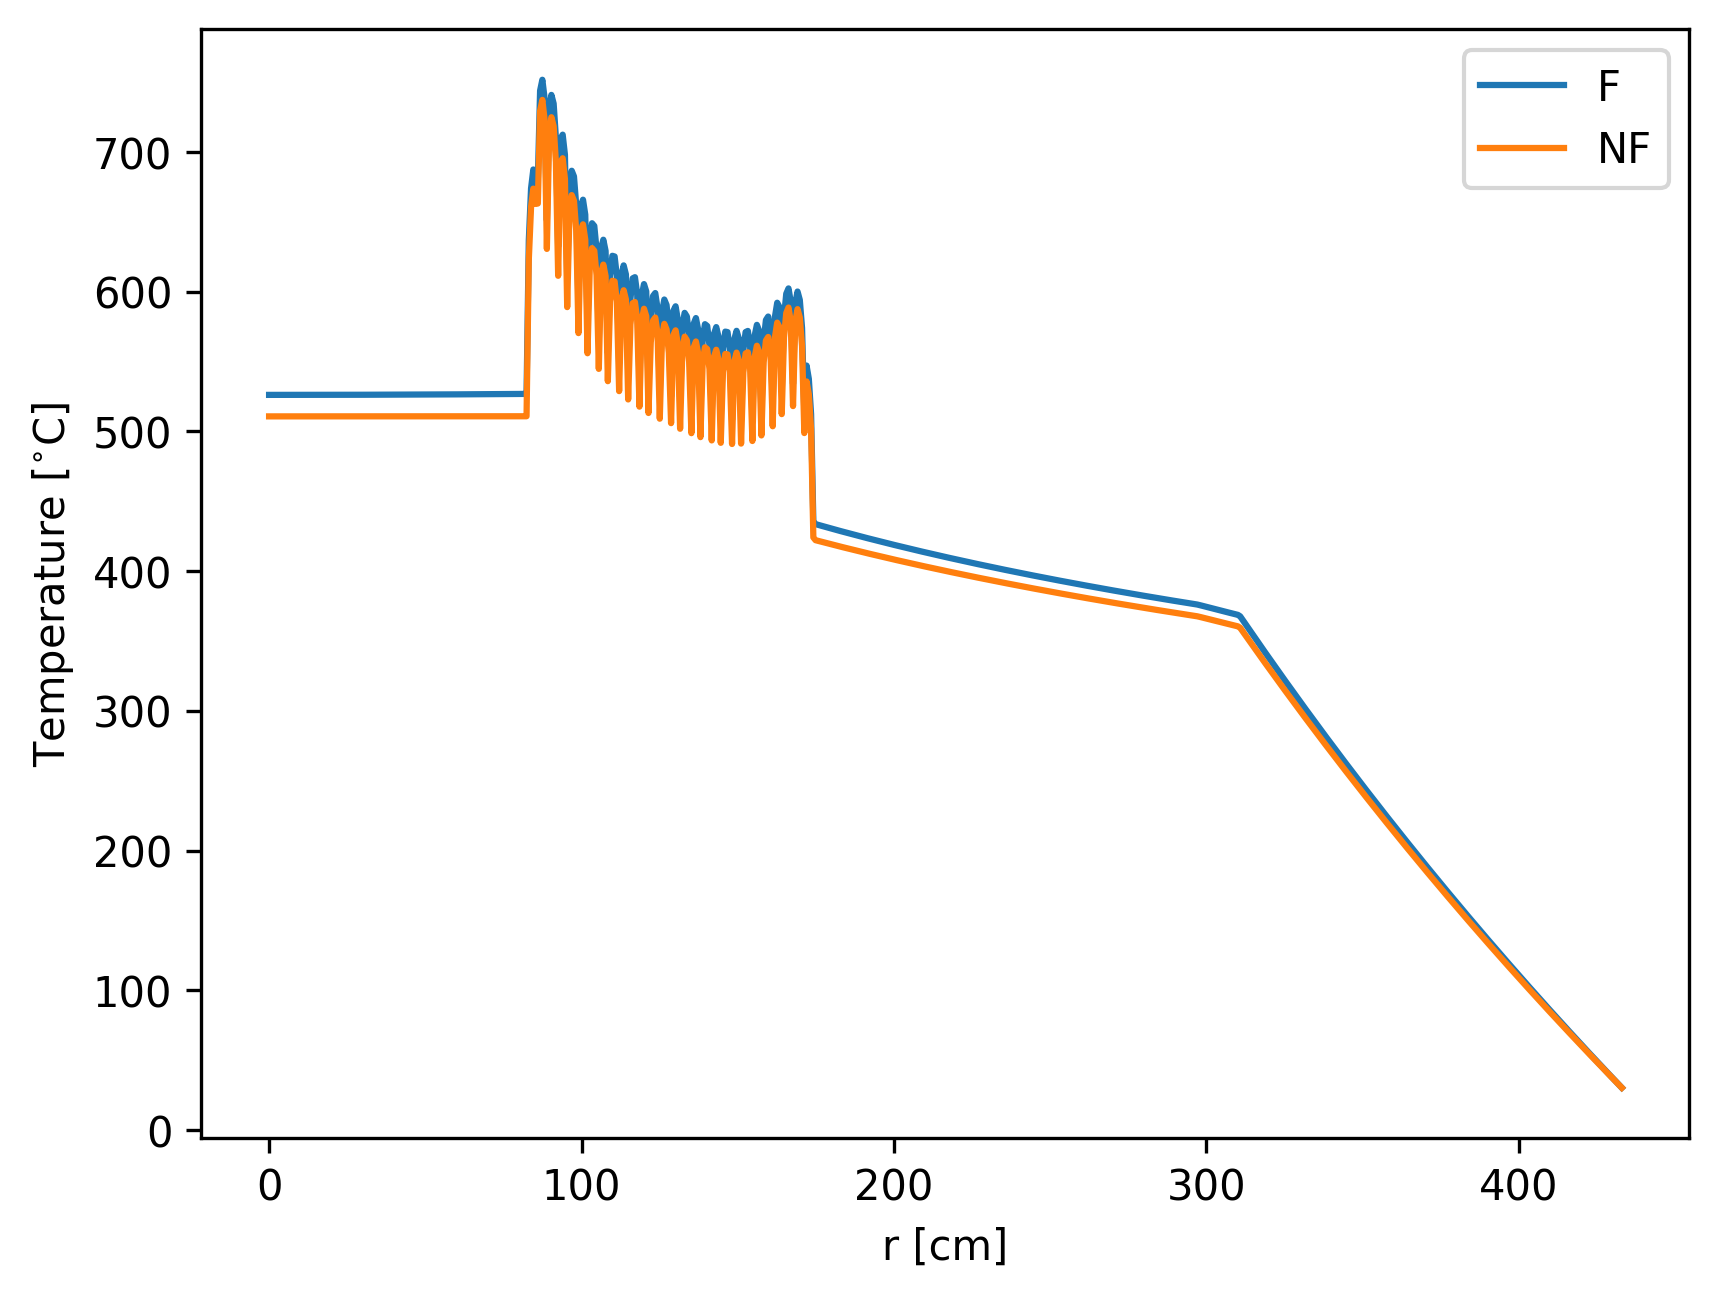
\includegraphics[width=0.45\textwidth]{figures-thermal/coupledD-3G-radialT}
    }
  \hfill
  \caption{Temperature profile comparison. F: thermal feedback, NF: no thermal feedback.}
  \label{fig:coupled-results-th}
\end{figure}

\subsection{Discussion}
\label{sec:discuss}

This section analyzes Moltres' flaws at conducting prismatic HTGR coupled simulations.
% Describe moltres heterogenous capabilities as an MSR solver
Moltres' initial development targeted MSRs, allowing it to rely on heterogeneous diffusion calculations.
In a heterogeneous solver, each mesh node holds the information of each variable.
In an MSR simulation, Moltres defines the neutron flux and the temperature on each node, and each node uses its temperature to compute the thermal feedback on the neutron flux.

% Moltres should use average temperatures
As discussed in Chapter \ref{ch:neutronics}, in a prismatic HTGR simulation, the neutronics calculation requires an assembly-level homogenization of the group constants.
Because of the homogenization, a mesh node holds the group constants' combined information from the different materials in the assembly --- only the fuel and the moderator as the coolant does not contribute considerably.
As the fuel group constants depended on the fuel temperature, and the moderator group constants depended on the moderator temperature, the thermal feedback depends on both temperatures.
Hence, a mesh node should hold both temperatures.

Section \ref{sec:ph1ex3} used a heterogeneous thermal-fluid model to solve the temperature in the reactor.
The problem with using a heterogeneous model is that each node only holds the temperature's value in that particular material.
A coolant node holds the coolant temperature information and computes the thermal feedback with such information instead of the moderator and fuel temperature.
For this reason, Moltres should use the average assembly-level fuel and moderator temperatures instead of the point-wise temperature to compute the thermal feedback.

% Moltres should differentiate Tmod and Tfuel
The thermal-fluids model in Section \ref{sec:ph1ex3} homogenized the fuel and the moderator into one material.
Such homogenization assumes that both the moderator and fuel are in thermal equilibrium, and therefore have the same temperature.
Consequently, the model does not differentiate the fuel temperature from the moderator temperature.
However, a coupling model cannot correctly calculate the thermal feedback if it does not differentiate between the moderator and the fuel temperatures \cite{damian_vhtr_2008}.

I denominate this issue as the 'homogenization dilemma.'
To correctly compute neutronics, the diffusion solver must use homogenized parameters which depend on both moderator and fuel temperatures.
Simultaneously, to accurately calculate the thermal feedback, a mesh node should differentiate the moderator temperature from the fuel temperature, which require a heterogeneous calculation in the thermal-fluids model.
A thermal-fluid heterogeneous calculation is still valid, but the thermal feedback should use fuel and moderator average temperatures instead.

\subsection{Coupled exercise with average temperature thermal feedback}
\label{sec:coupled-average}

The previous discussion led to the development of this section.
This section conducted Section \ref{sec:ph1ex3} analysis calculating the thermal feedback with the solid average temperatures.
Section \ref{sec:ph1ex3} calculated the thermal feedback using the point-wise temperatures.
This section compares the results from both approaches.

Figure \ref{fig:coupled-ave-results-th2} exhibits the point-wise temperature and the average temperatures across the reactor.
The model used the average temperatures to compute the thermal feedback in the core.
The simulations did not compute the average temperature in the RPV and the outside air.
Figure \ref{fig:coupled-ave-results-flux} displays the neutron flux profiles, and Figure \ref{fig:coupled-ave-results-th}, the temperature profiles.
The results are almost identical.
The only noticeable difference is in the axial temperature profile, which differ by less than 3$^{\circ}$C in the outlet.
The radial temperature profile is not affected.

This analysis expected more variations in the results.
The point-wise approach arrived at similar results because the difference between the solid and coolant temperature is small (less than 100$^{\circ}$C).
However, in transient analyses, the temperature difference between the fuel and the coolant may increase, causing more variability in the results.
% Although using the point-wise approach is easier for the input file definition, 
Further studies should analyze this behavior.

\begin{figure}[htbp!]
  \centering
    \subfloat[Temperature profile.]{
        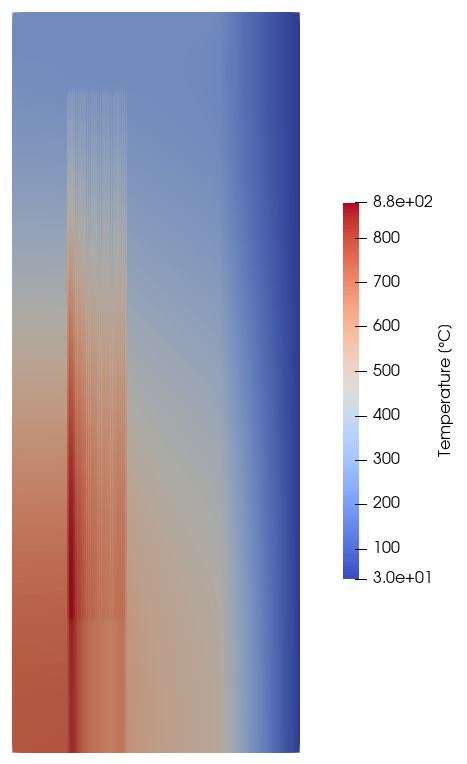
\includegraphics[width=0.40\textwidth]{figures-thermal/coupledH-temp}
    }
    \subfloat[Average temperature in each assembly.]{
        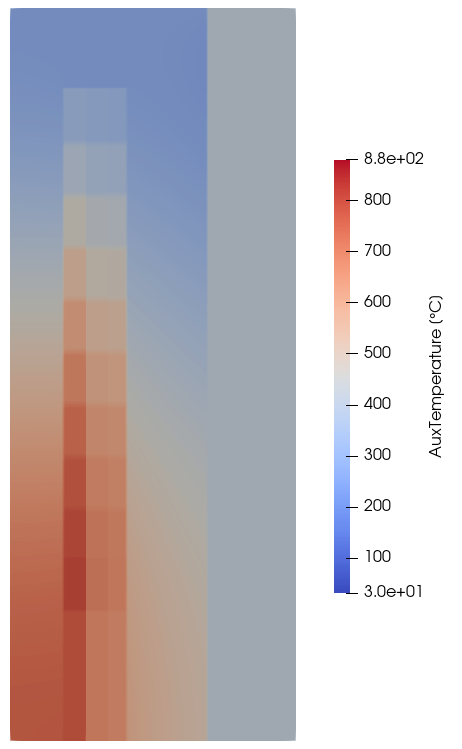
\includegraphics[width=0.40\textwidth]{figures-thermal/coupledH-auxtemp}
    }
  \hfill
  \caption{Temperature distribution.}
  \label{fig:coupled-ave-results-th2}
\end{figure}

\begin{figure}[htbp!]
  \centering
    \subfloat[Axial flux over the line at r=85 cm.]{
        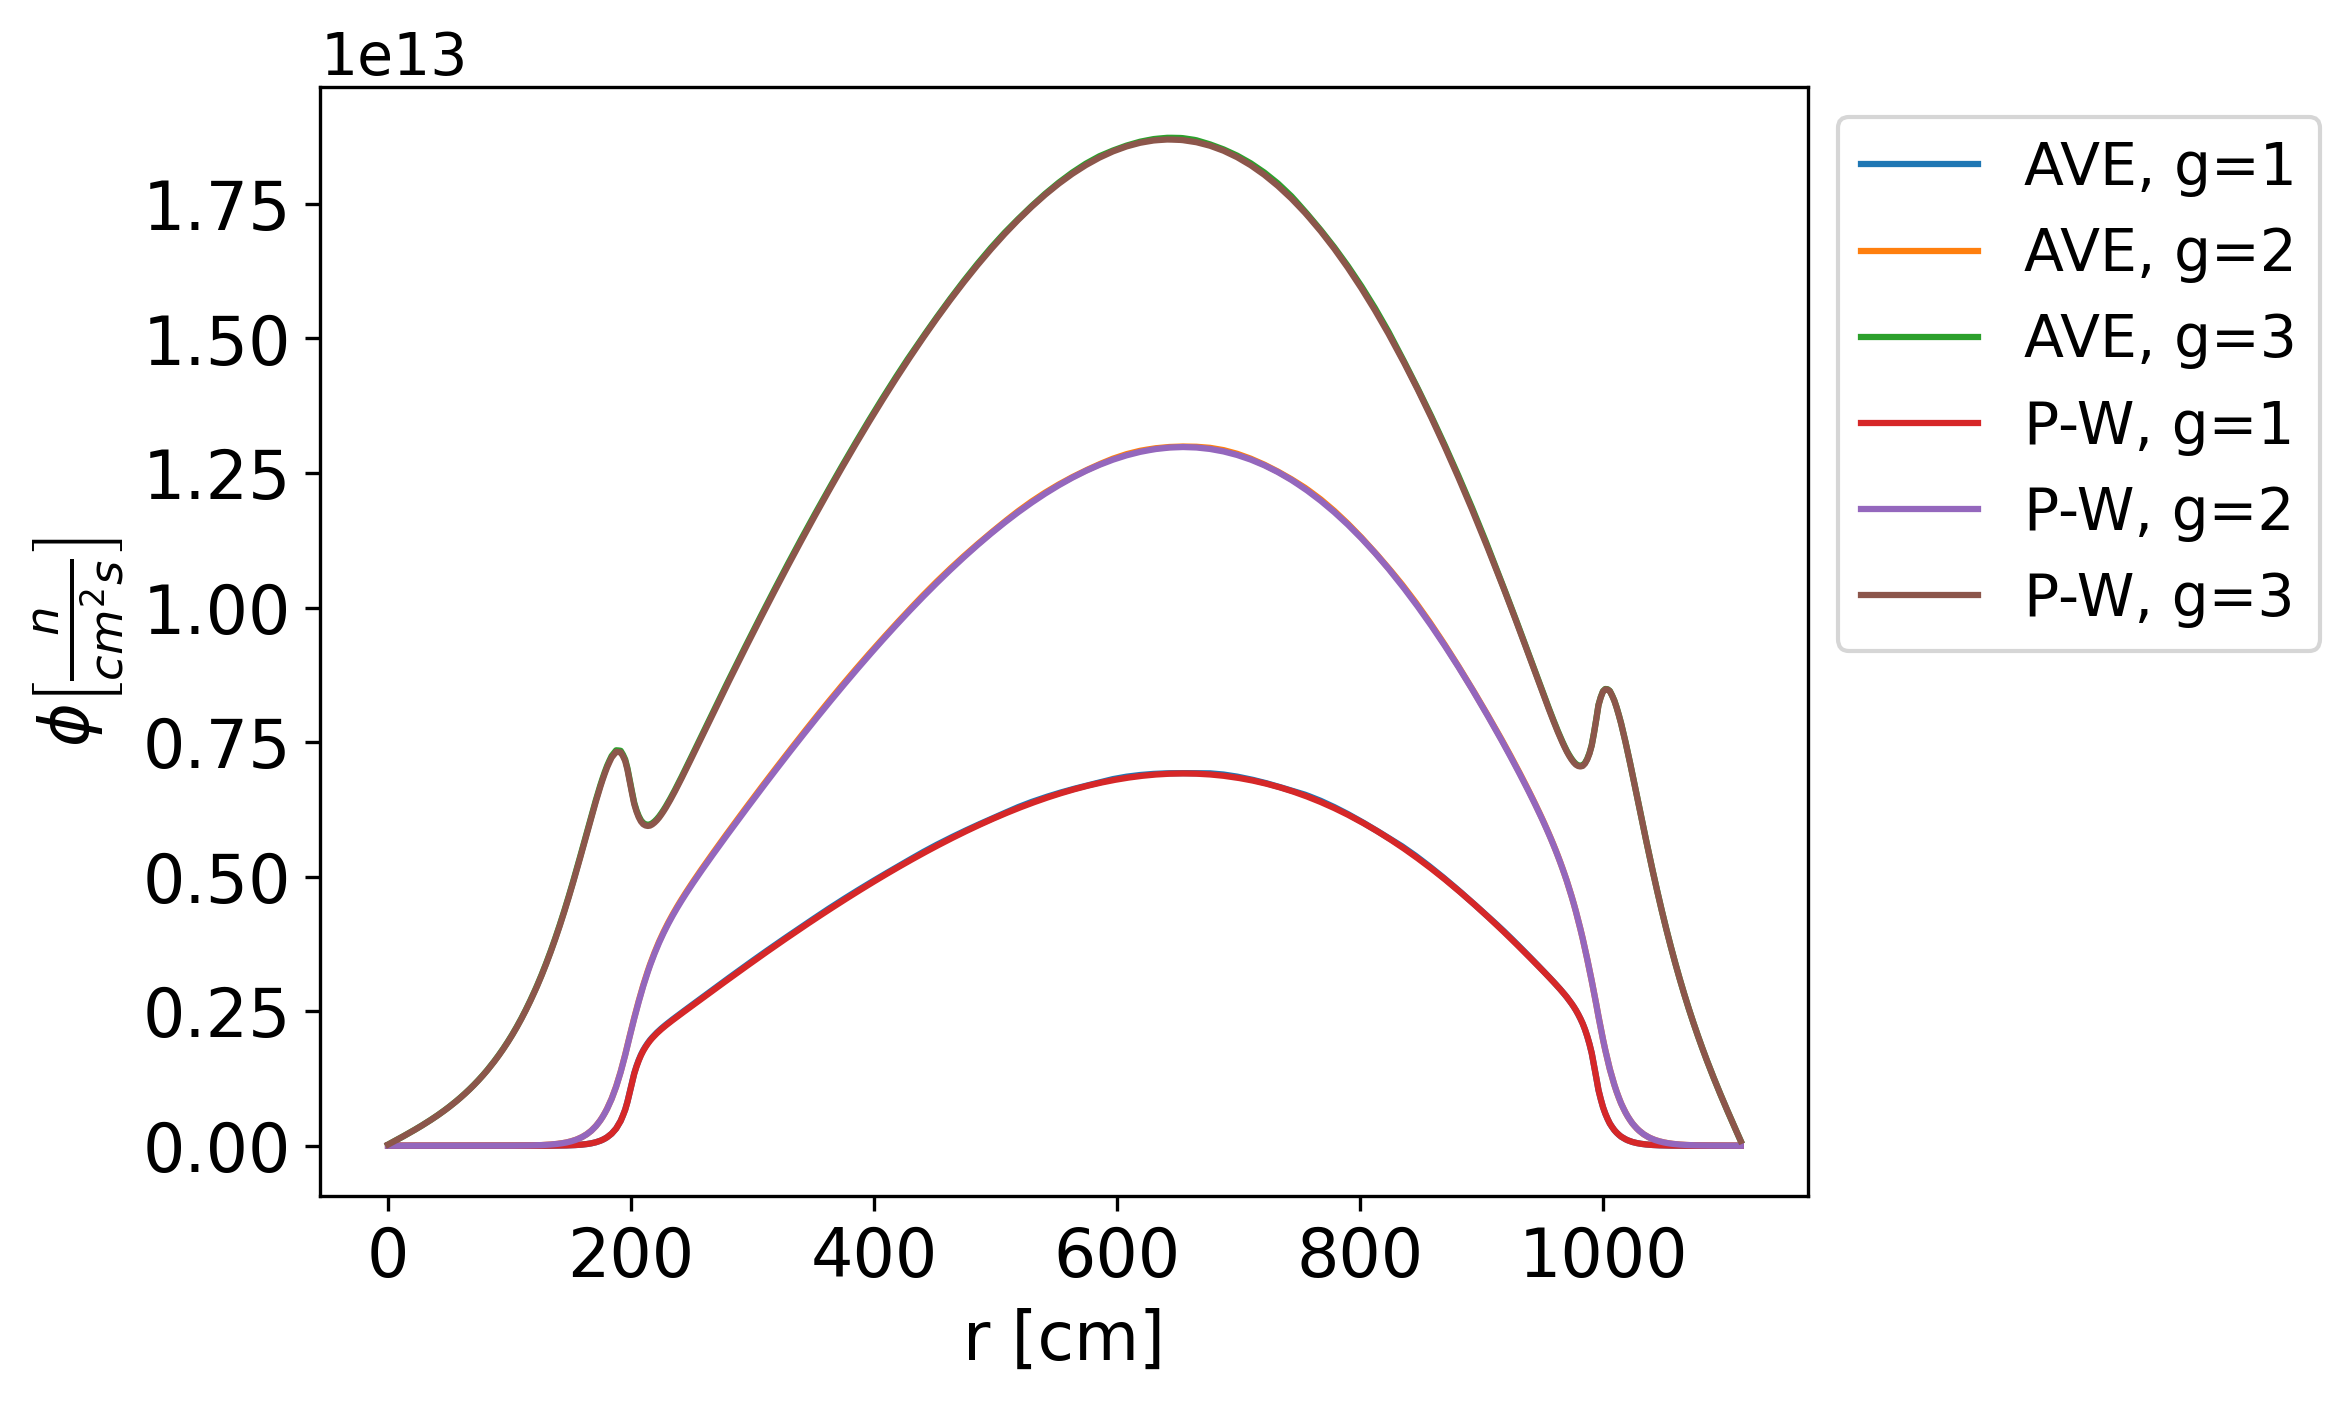
\includegraphics[width=0.45\textwidth]{figures-thermal/coupledD-H-axial}
    }
    \subfloat[Radial temperature at z=L/2=556.5 cm]{
        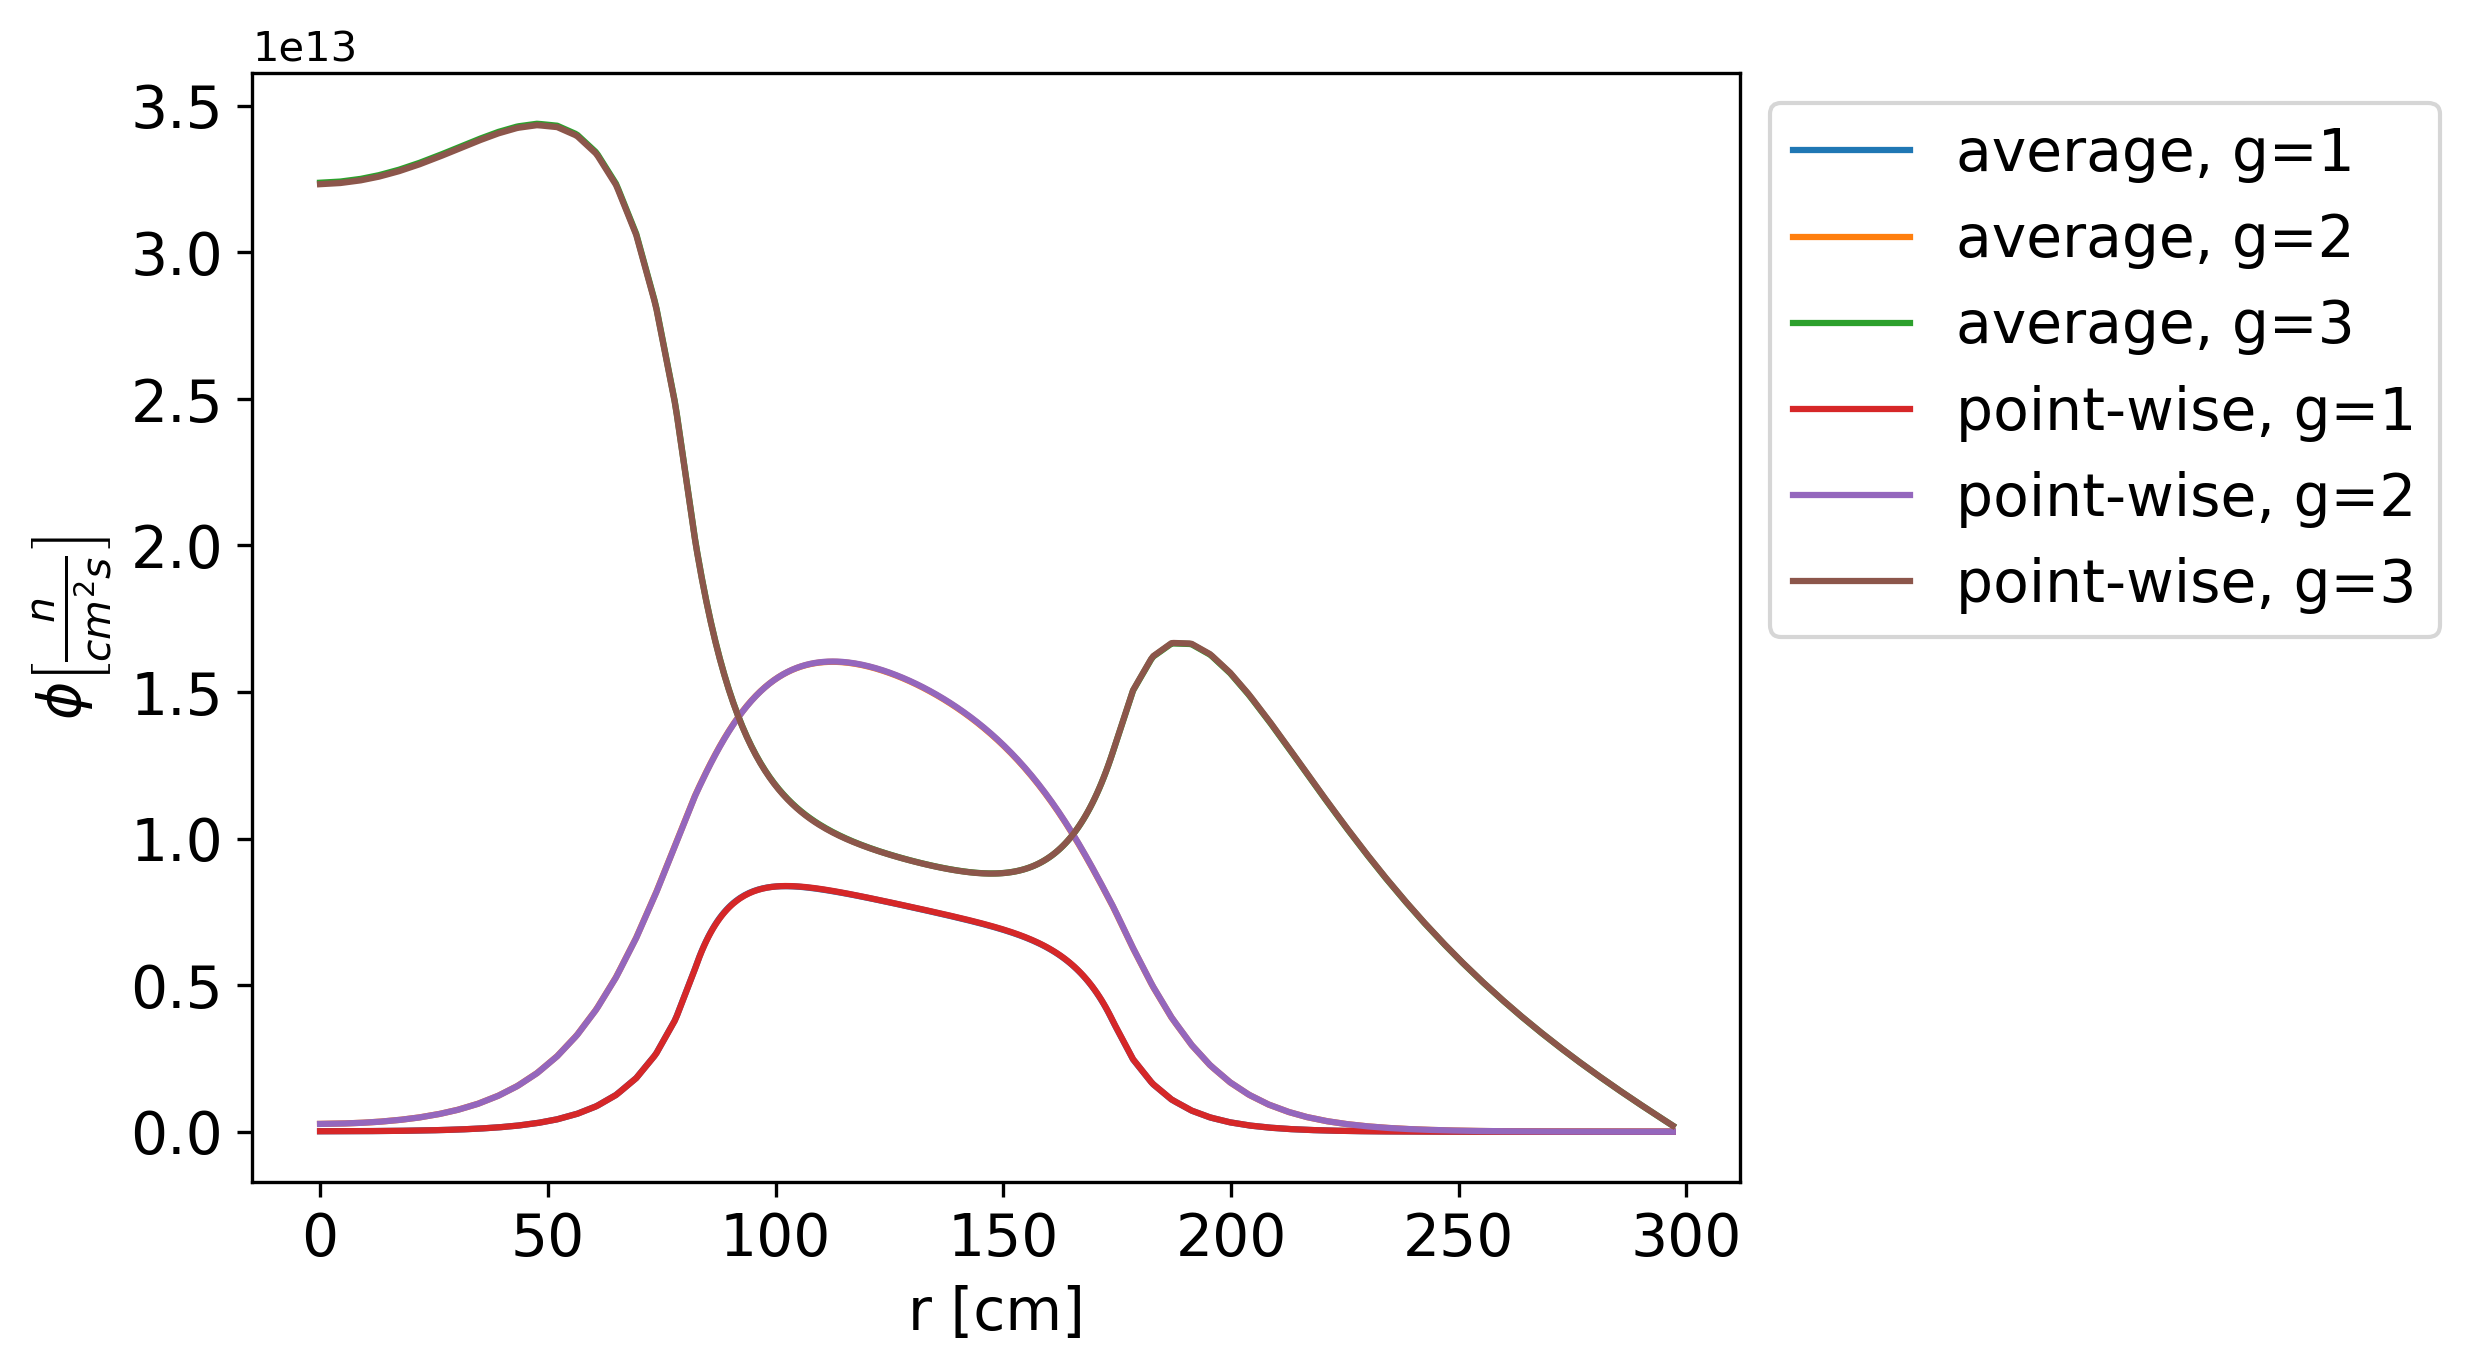
\includegraphics[width=0.45\textwidth]{figures-thermal/coupledD-H-radial}
    }
  \hfill
  \caption{Flux profile comparison.}
  \label{fig:coupled-ave-results-flux}
\end{figure}

\begin{figure}[htbp!]
  \centering
    \subfloat[Axial temperature at r=85 cm.]{
        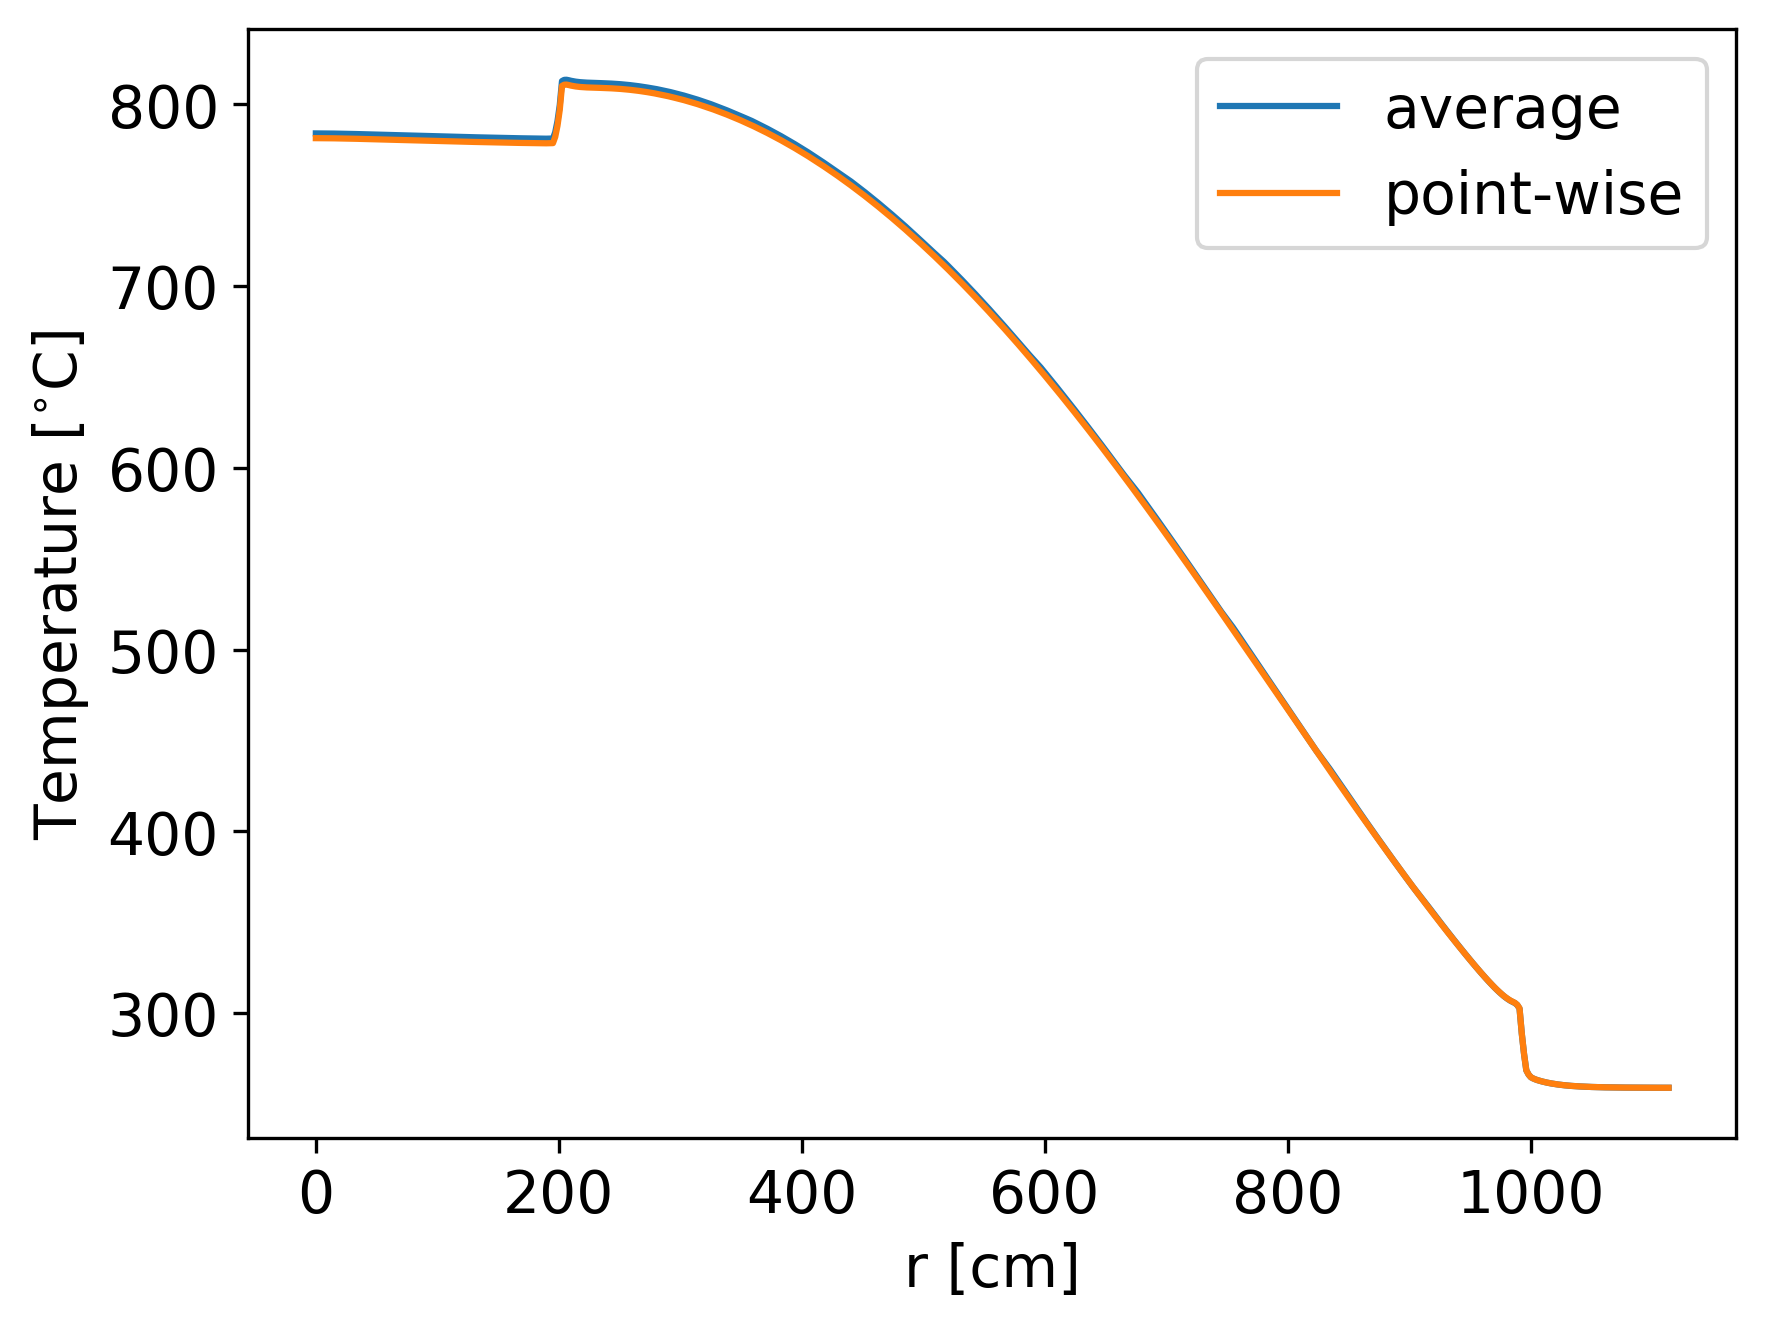
\includegraphics[width=0.45\textwidth]{figures-thermal/coupledD-H-axialT}
    }
    \subfloat[Radial temperature at z=L/2=556.5 cm]{
        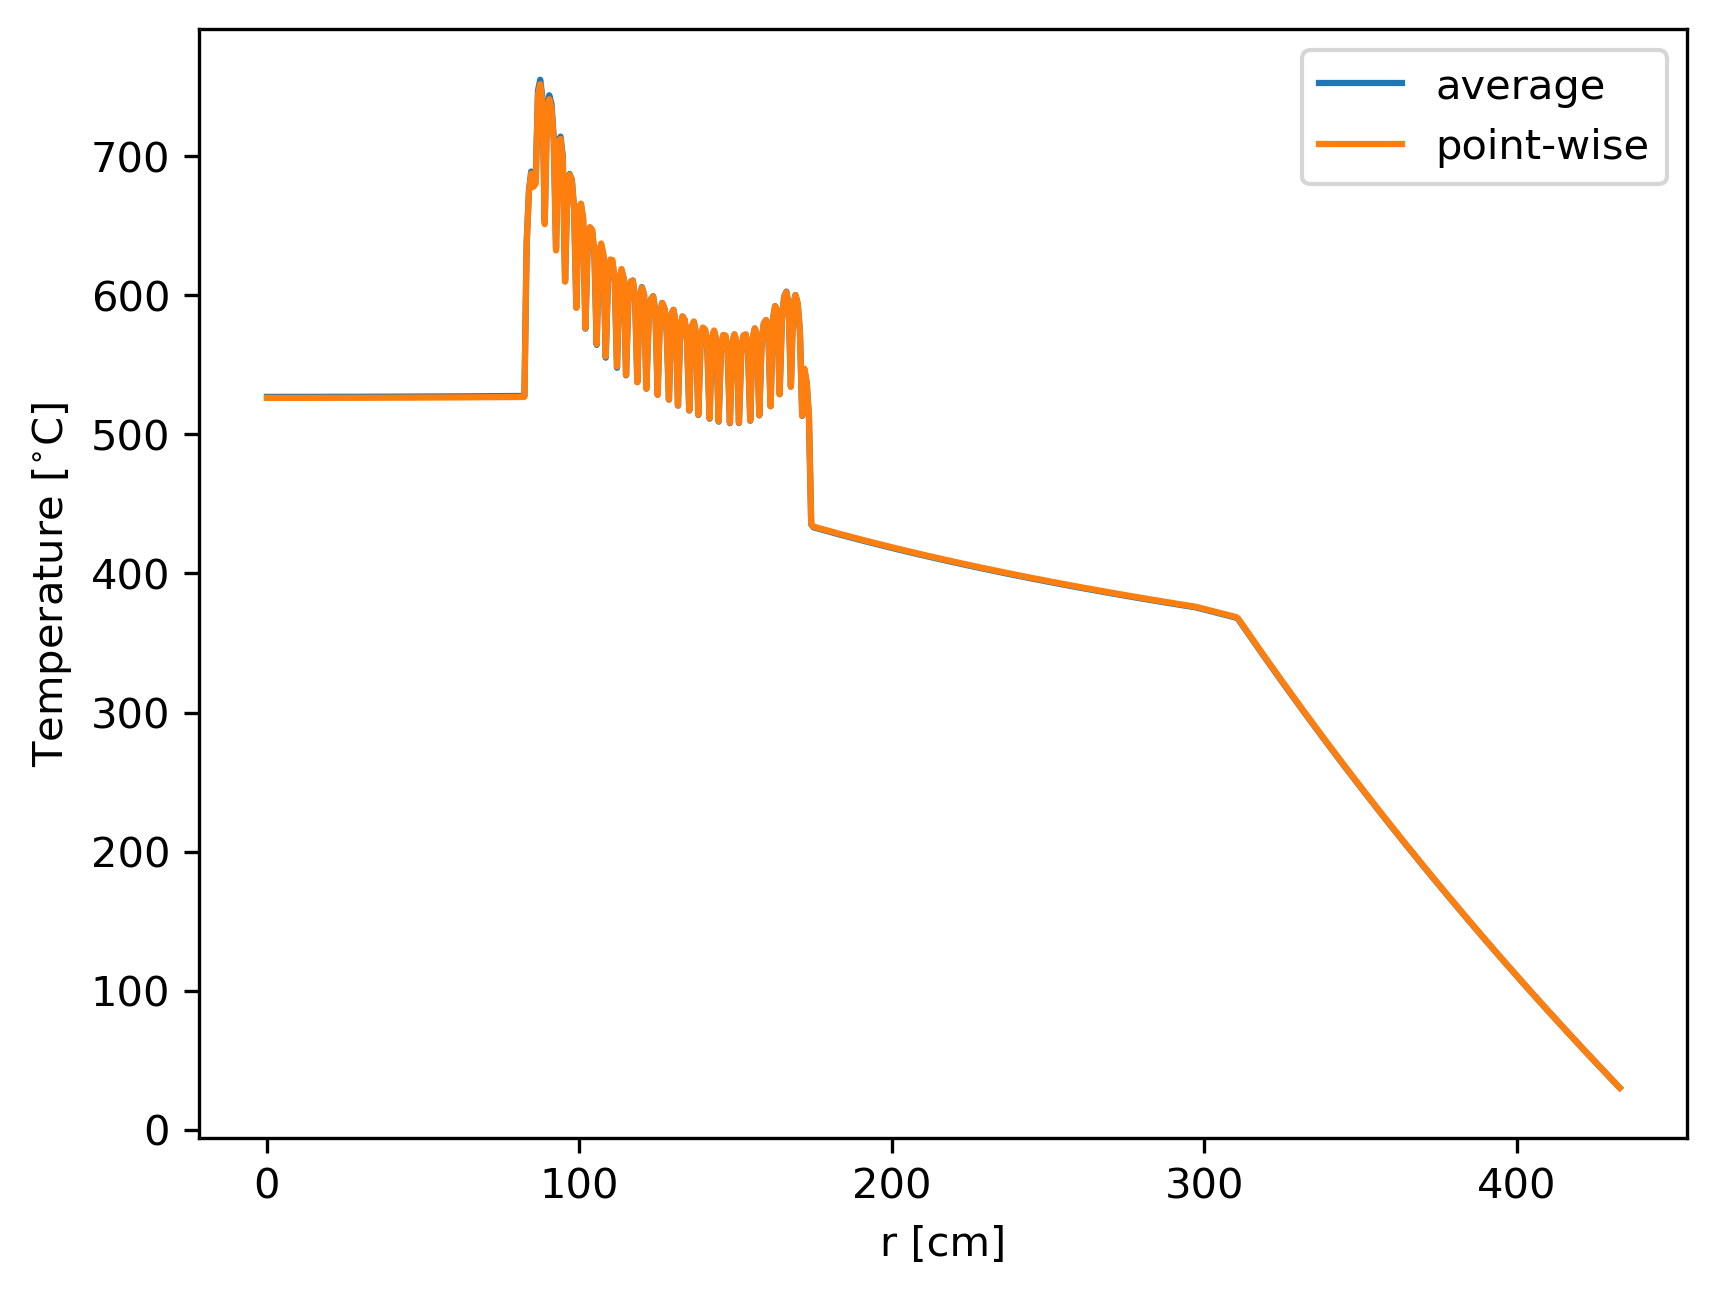
\includegraphics[width=0.45\textwidth]{figures-thermal/coupledD-H-radialT}
    }
  \hfill
  \caption{Temperature profile comparison.}
  \label{fig:coupled-ave-results-th}
\end{figure}

\section{Conclusions}
\label{sec:thermal-conc}

The preliminary studies focused on the verification of the thermal-fluids model and the validation of the unit-cell model.
The verification of the thermal-fluids model studied a simplified cylindrical model comparing the Moltres/MOOSE numerical solution to the problem analytical solution - both solutions were in agreement.
This study set the basis for the unit cell problem set-up.
% The unit cell problem use thermal-fluids model from the previous verification.
To validate the unit cell model, Section \ref{sec:unitcell} compared Moltres/MOOSE results to the results of In et al. \cite{in_three-dimensional_2006}.
The results presented some discrepancies: the outlet coolant and moderator temperatures differed by less than 10$^{\circ}$C, while the fuel temperature differed by 22$^{\circ}$C.
We expected some variability in the results as some of our simulation parameters may have varied from the original study.
In's article is missing the materials definition, so Section \ref{sec:unitcell} adopted the material properties from Tak et al. \cite{tak_numerical_2008}.
Additionally, In used a chopped cosine power profile, while the Section \ref{sec:unitcell} model simplified the calculation using a uniform power density.

The Section \ref{sec:fuelcol} focus of the analysis was a one-twelfth section of an HTGR fuel column.
To validate the model, Section \ref{sec:fuelcol} intended to reproduce Sato et al. \cite{sato_computational_2010} results.
Section \ref{sec:fuelcol} conducted two studies: one with no bypass-gap, and one with a 3mm-bypass-gap.
To simplify the analysis, our model adopted the mass flow rates from Sato's article.
For both case studies, the maximum temperatures in the coolant and the fuel showed good agreement.
Section \ref{sec:fuelcol} also presented the temperature profile in two of the edges of the geometry.
Such an analysis exhibits the effects of the bypass flow on the temperature.
The presence of the gap makes the center temperature rise while it reduces the peripheral temperature.
The overall consequence is an increase in the temperature gradient inside the column.

The next analysis studied different calculation methods for the mass flow distribution in the fuel column.
Section \ref{sec:flowdistrib} adopted Sato's mass flow distribution as the reference value and calculated the mass flow distribution using four different methods.
From Case 2 to Case 5, the methods' complexity increased as some required iterative solvers.
Overall, Case 2 proved to be the simplest method, and its application did not considerably deteriorate the results' accuracy.
For that reason, the following studies adopted the Case 2 mass flow distribution method.

Keeping in mind that the ultimate objective of this work is to conduct full-scale simulations, Section \ref{sec:meshconverge} studied the feasibility of extending this methodology to larger meshes.
Section \ref{sec:meshconverge} conducted a mesh convergence analysis on the full-fuel column problem.
As the model uses the one-dimensional coolant equations, the coolant temperature converges relatively fast compared to the fuel temperature.
The fuel temperature did not reach convergence in this analysis as the mesh discretization increase imposed a high memory requirement on the simulations.
This analysis concluded that modeling thermal-fluids with such a detailed level is computationally too expensive, and it suggests searching for other methods.
The following sections adopted a two-dimensional cylindrical model for the full-core analyses.

Section \ref{sec:ph1ex2} described Phase I Exercise 2 of the OECD/NEA MHTGR-350 Benchmark.
This exercise encompasses four sub-cases with different definitions of bypass-flow and material properties.
The simplest exercise is Exercise 2a, as it does not model the bypass flow and provides the definition of the material properties.
Section \ref{sec:ph1ex2} used Moltres/MOOSE to conduct Exercise 2a.
Additionally, the Moltres thermal-fluids model bases its definition on INL's model.
As OECD/NEA did not publish this exercise’s results, Section \ref{sec:ph1ex2} compared Moltres/MOOSE results to INL benchmark results \cite{strydom_inl_2013}.
The large discrepancies between Moltres/MOOSE and INL results suggest that our model does not capture some heat transfer mechanism that the INL model does.
One of the known differences between the models is the inclusion of the radiative heat transfer mechanism.
As Moltres does not model that mechanism, it could be the cause of the differences.

Section \ref{sec:ph1ex2} used a global and a unit cell model based on Stainsby's approach \cite{stainsby_investigation_2008} to circumvent this drawback.
The global model is responsible for calculating the coolant temperature, while the unit cell model focuses on the moderator and fuel temperatures.
With this approach, Moltres/MOOSE results were closer to INL results.
The results showed some discrepancies, which indicates that some assumption/model simplification is not accurate enough.
A flat velocity approximation might be the cause of such discrepancies.
Further studies should analyze the origin of the discrepancies.

Section \ref{sec:ph1ex3} developed a global model to solve a simplified version of Phase 1 Exercise 3 of the OECD/NEA benchmark.
Although the model was simple, it allowed visualizing some of the essential aspects of a prismatic HTGR multi-physics simulation in Moltres.
This exercise led to Section \ref{sec:discuss}, which described some of the flaws found in the model.
Additionally, Section \ref{sec:coupled-average} addressed some of the flaws found in the model and set the basis for conducting prismatic HTGR coupled exercises in Moltres.
% This exercise also sets the basis for future work that Section \ref{sec:futwork} will introduce.
